\documentclass[
    12pt,
    a4paper,
    oneside
]{report}

\usepackage[utf8]{inputenc}
\usepackage[T1]{fontenc}
\usepackage[brazilian]{babel}
\usepackage{lmodern}
\usepackage{microtype}

\usepackage[a4paper,margin=2.5cm]{geometry}
\usepackage{setspace}
\onehalfspacing

\usepackage{amsmath,amssymb}
\usepackage{graphicx}
\usepackage{float}
\usepackage{caption}
\usepackage{subcaption}
\usepackage{booktabs}
\usepackage{array}
\usepackage{longtable}
\usepackage{siunitx}
\sisetup{
    output-decimal-marker={,},
    detect-all=true
}

\usepackage{xcolor}
\definecolor{codigoFundo}{RGB}{248,248,248}
\definecolor{codigoBorda}{RGB}{210,210,210}
\definecolor{codigoComentario}{RGB}{70,120,70}
\definecolor{codigoString}{RGB}{150,70,70}
\definecolor{codigoKeyword}{RGB}{20,70,140}

\usepackage{listings}
\lstdefinestyle{codigoC}{
    language=C,
    basicstyle=\ttfamily\scriptsize,
    keywordstyle=\color{codigoKeyword}\bfseries,
    commentstyle=\color{codigoComentario},
    stringstyle=\color{codigoString},
    numbers=left,
    numberstyle=\tiny\color{gray},
    stepnumber=1,
    numbersep=8pt,
    frame=single,
    rulecolor=\color{codigoBorda},
    backgroundcolor=\color{codigoFundo},
    breaklines=true,
    breakatwhitespace=false,
    postbreak=\mbox{\textcolor{gray}{$\hookrightarrow$}\space},
    tabsize=4,
    showstringspaces=false,
    keepspaces=true,
    columns=fullflexible,
    captionpos=b,
    inputencoding=utf8,
    extendedchars=true,
    literate=
        {á}{{\'a}}1 {à}{{\`a}}1 {ã}{{\~a}}1 {â}{{\^a}}1
        {Á}{{\'A}}1 {À}{{\`A}}1 {Ã}{{\~A}}1 {Â}{{\^A}}1
        {é}{{\'e}}1 {ê}{{\^e}}1 {É}{{\'E}}1 {Ê}{{\^E}}1
        {í}{{\'i}}1 {Í}{{\'I}}1
        {ó}{{\'o}}1 {õ}{{\~o}}1 {ô}{{\^o}}1
        {Ó}{{\'O}}1 {Õ}{{\~O}}1 {Ô}{{\^O}}1
        {ú}{{\'u}}1 {Ú}{{\'U}}1
        {ç}{{\c{c}}}1 {Ç}{{\c{C}}}1
        {º}{{$^\circ$}}1 {ª}{{$^a$}}1
        {²}{{$^2$}}1 {³}{{$^3$}}1
        {∫}{{$\int$}}1 {≤}{{$\le$}}1 {≥}{{$\ge$}}1
        {–}{{--}}1 {—}{{--}}1
}

\lstset{style=codigoC}

\usepackage{tikz}
\usetikzlibrary{arrows.meta,positioning,shapes.geometric,fit,calc}
\tikzset{
    bloco/.style={
        rectangle,
        draw,
        rounded corners=2pt,
        align=center,
        minimum height=0.8cm,
        text width=3.2cm
    },
    processo/.style={bloco, fill=blue!5},
    decisao/.style={
        diamond,
        draw,
        align=center,
        aspect=2,
        inner sep=1pt,
        fill=yellow!10
    },
    fluxo/.style={-{Latex[length=2mm]}, thick},
    componente/.style={bloco, fill=gray!8},
    thread/.style={bloco, fill=green!8},
    regiaoParalela/.style={draw, dashed, rounded corners=3pt, inner sep=6pt}
}

\usepackage{pgfplots}
\pgfplotsset{compat=1.18}

\usepackage[most]{tcolorbox}
\newtcolorbox{conceitobox}{
    colback=blue!3,
    colframe=blue!40!black,
    boxrule=0.4pt,
    arc=2pt,
    left=6pt,
    right=6pt,
    top=6pt,
    bottom=6pt
}
\newtcolorbox{decisionbox}{
    colback=orange!4,
    colframe=orange!45!black,
    boxrule=0.4pt,
    arc=2pt,
    left=6pt,
    right=6pt,
    top=6pt,
    bottom=6pt
}
\newtcolorbox{validationbox}{
    colback=green!4,
    colframe=green!40!black,
    boxrule=0.4pt,
    arc=2pt,
    left=6pt,
    right=6pt,
    top=6pt,
    bottom=6pt
}
\newtcolorbox{oralbox}{
    colback=gray!5,
    colframe=gray!55,
    boxrule=0.4pt,
    arc=2pt,
    left=6pt,
    right=6pt,
    top=6pt,
    bottom=6pt
}

\usepackage{csquotes}
\usepackage[
    backend=biber,
    style=numeric,
    sorting=none
]{biblatex}
\addbibresource{referencias.bib}

\usepackage[
    hidelinks,
    plainpages=false,
    pdfpagelabels
]{hyperref}
\usepackage[nameinlink,noabbrev]{cleveref}


\begin{document}

\hypersetup{pageanchor=false}

\begin{titlepage}
    \centering

    {\Large Universidade Federal do Rio Grande do Norte\par}
    \vspace{0.3cm}

    {\large Instituto Metrópole Digital\par}

    \vfill

    {\Huge\bfseries Relatório Final da Primeira Unidade\par}

    \vspace{0.4cm}

    {\LARGE Computação de Alto Desempenho\par}

    \vspace{1cm}

    {\large Relatórios das atividades práticas e experimentais\par}

    \vfill

    {\Large\bfseries Douglas Felipe\par}

    \vfill

    {\large Natal -- RN\par}
    {\large 2026\par}
\end{titlepage}

\pagenumbering{roman}

\tableofcontents
\clearpage

\listoffigures
\clearpage

\listoftables
\clearpage

\pagenumbering{arabic}
\hypersetup{pageanchor=true}

\chapter*{Introdução}
\addcontentsline{toc}{chapter}{Introdução}

Este documento reúne os relatórios das atividades desenvolvidas na primeira unidade da disciplina de Computação de Alto Desempenho.
Cada atividade será documentada, posteriormente, em termos teóricos, metodológicos e experimentais.
Nesta versão inicial, o relatório estabelece a estrutura modular do documento e incorpora os códigos-fonte desenvolvidos nas atividades.

% ============================================================
% DEPENDÊNCIAS DESTE CAPÍTULO
%
% Adicionar ao preâmbulo do documento principal, caso ainda
% não estejam presentes:
%
% \usepackage{booktabs}
% \usepackage{longtable}
% \usepackage{float}
% \usepackage{tikz}
% \usepackage{pgfplots}
%
% \usetikzlibrary{
%     arrows.meta,
%     positioning,
%     shapes.geometric
% }
%
% \pgfplotsset{compat=1.18}
% ============================================================


\chapter{Atividade 1 -- Multiplicação matriz por vetor e acesso a memória}

\label{chap:atvd01}


% ============================================================
% ENUNCIADO
% ============================================================

\section{Enunciado da tarefa}

\label{sec:atvd01-enunciado}

\begin{quote}

Implemente duas versões da multiplicação de matriz por vetor (MxV) em C:
uma versão com acesso a matriz por linhas, utilizando linha externa e
coluna interna; outra versão com acesso a matriz por colunas, utilizando
coluna externa e linha interna.

Meça o tempo de execução de cada versão utilizando uma função apropriada
de temporização e execute testes com diferentes tamanhos de matriz.

Identifique a partir de que tamanho os tempos das duas implementações
passam a divergir significativamente e explique por que isso ocorre,
relacionando as observações com o uso da memória cache e o padrão de
acesso a memória.

\end{quote}


% ============================================================
% OBJETIVOS
% ============================================================

\section{Objetivos e requisitos}

\label{sec:atvd01-objetivos}

A atividade tem como objetivo avaliar experimentalmente o impacto do
padrão de acesso à memória sobre o desempenho da multiplicação
matriz-vetor.

As duas implementações executam a mesma operação matemática e possuem a
mesma complexidade assintótica, diferindo essencialmente na ordem em que
os elementos da matriz são percorridos.

Os principais requisitos identificados para o experimento são:

\begin{itemize}

    \item implementar a multiplicação matriz-vetor com percurso da matriz
    por linhas;

    \item implementar a mesma operação com percurso da matriz por colunas;

    \item utilizar a mesma representação de dados nas duas versões;

    \item variar sistematicamente a dimensão da matriz;

    \item medir exclusivamente o trecho correspondente à multiplicação;

    \item utilizar uma fonte de tempo monotônica;

    \item realizar múltiplas medições para reduzir a influência de ruído
    experimental;

    \item validar a equivalência funcional entre as duas implementações;

    \item apresentar os tempos de forma comparável;

    \item calcular uma métrica adicional que represente diretamente a
    diferença entre os dois padrões de acesso;

    \item relacionar os resultados obtidos com localidade espacial,
    stride de memória e hierarquia de cache.

\end{itemize}

Como métrica comparativa adicional foi definida a razão:

\begin{equation}
    C/L =
    \frac{T_{\mathrm{coluna}}}
         {T_{\mathrm{linha}}},
    \label{eq:atvd01-cl}
\end{equation}

em que \(T_{\mathrm{coluna}}\) representa o tempo da implementação com
percurso por colunas e \(T_{\mathrm{linha}}\) representa o tempo da
implementação com percurso por linhas.

A interpretação da métrica é direta:

\begin{itemize}

    \item \(C/L \approx 1\): tempos semelhantes;

    \item \(C/L > 1\): a versão por colunas apresenta maior tempo;

    \item \(C/L < 1\): a versão por colunas apresenta menor tempo na
    medição considerada.

\end{itemize}


% ============================================================
% FUNDAMENTAÇÃO
% ============================================================

\section{Fundamentação conceitual}

\label{sec:atvd01-fundamentacao}

\subsection{Multiplicação matriz-vetor}

Considere uma matriz quadrada \(A\) de dimensão \(N \times N\), um vetor
\(x\) com \(N\) elementos e um vetor resultado \(y\).

A multiplicação matriz-vetor é definida por:

\begin{equation}
    y_i =
    \sum_{j=0}^{N-1}
    A_{ij}x_j,
    \qquad
    i = 0,1,\ldots,N-1.
    \label{eq:atvd01-mxv}
\end{equation}

Para cada posição do vetor de saída é calculado o produto interno entre
uma linha da matriz e o vetor de entrada.

As duas implementações avaliadas realizam aproximadamente \(N^2\)
multiplicações e \(N^2\) acumulações. Portanto, ambas apresentam
complexidade assintótica:

\begin{equation}
    O(N^2).
\end{equation}

A atividade não compara algoritmos com ordens de complexidade distintas.
O aspecto central é a diferença entre os padrões de acesso aos dados.


\subsection{Organização row-major}

Na representação utilizada pelo programa, a matriz é armazenada em um
único bloco contínuo de memória.

O elemento lógico:

\begin{equation}
    A[i][j]
\end{equation}

é acessado por:

\begin{equation}
    A[i \times N + j].
    \label{eq:atvd01-rowmajor}
\end{equation}

Essa representação corresponde à organização \textit{row-major}, em que
os elementos pertencentes a uma mesma linha ocupam posições consecutivas
na memória.

Assim, a sequência:

\begin{verbatim}
A[i][0], A[i][1], A[i][2], ...
\end{verbatim}

corresponde a acessos contíguos.

Por outro lado, a sequência:

\begin{verbatim}
A[0][j], A[1][j], A[2][j], ...
\end{verbatim}

realiza saltos entre posições pertencentes a linhas diferentes.


\subsection{Localidade espacial}

A hierarquia de memória transfere dados em blocos, e não necessariamente
um elemento isolado por acesso.

Quando um programa utiliza uma posição de memória, elementos próximos
também podem ser disponibilizados em níveis rápidos da hierarquia.

O percurso por linhas explora esse comportamento porque os elementos
subsequentes da linha estão armazenados em posições adjacentes.

Esse comportamento é associado à \textbf{localidade espacial}.


\subsection{Stride de memória}

O \textit{stride} representa a distância, em bytes, entre endereços
sucessivos acessados por uma determinada sequência de execução.

Na implementação por linhas, utilizando dados do tipo \texttt{int}, o
stride principal sobre a matriz é aproximadamente:

\begin{equation}
    S_{\mathrm{linha}} = sizeof(int).
\end{equation}

No ambiente utilizado:

\begin{equation}
    sizeof(int) = 4\ \text{bytes}.
\end{equation}

Portanto:

\begin{equation}
    S_{\mathrm{linha}} = 4\ \text{bytes}.
\end{equation}

Na implementação por colunas:

\begin{equation}
    S_{\mathrm{coluna}}
    =
    N \times sizeof(int).
    \label{eq:atvd01-stride}
\end{equation}

Por exemplo, para \(N=2000\):

\begin{equation}
    S_{\mathrm{coluna}}
    =
    2000 \times 4
    =
    8000\ \text{bytes}.
\end{equation}

Para \(N=5000\):

\begin{equation}
    S_{\mathrm{coluna}}
    =
    5000 \times 4
    =
    20000\ \text{bytes}.
\end{equation}

O aumento do stride reduz a capacidade de aproveitar imediatamente os
dados vizinhos carregados pela hierarquia de memória.


\subsection{Hierarquia de memória}

O desempenho observado depende da interação entre o padrão de acesso e
a hierarquia de memória:

\begin{verbatim}
Registradores
     |
Cache L1
     |
Cache L2
     |
Cache L3
     |
Memória principal
\end{verbatim}

Os níveis mais próximos do processador apresentam menor capacidade, mas
menor latência.

Conforme o conjunto de dados aumenta, uma parcela crescente dos acessos
pode depender de níveis mais distantes da hierarquia.

Entretanto, o tamanho nominal de uma cache não constitui, isoladamente,
um limiar rígido de desempenho. Associatividade, políticas de
substituição, prefetching, tradução de endereços e os demais dados
utilizados pelo programa também influenciam o comportamento observado.


% ============================================================
% INTERPRETAÇÃO DIDÁTICA
% ============================================================

\section{Interpretação didática da tarefa}

\label{sec:atvd01-interpretacao}

O aspecto didático central da atividade é demonstrar que a complexidade
assintótica não caracteriza sozinha o desempenho real de uma
implementação.

As duas versões executam a mesma multiplicação e possuem complexidade
\(O(N^2)\). Entretanto, a ordem dos laços modifica a sequência de
endereços acessados.

A versão por linhas apresenta o padrão:

\begin{verbatim}
A[0][0] -> A[0][1] -> A[0][2] -> ...
\end{verbatim}

enquanto a versão por colunas apresenta:

\begin{verbatim}
A[0][0] -> A[1][0] -> A[2][0] -> ...
\end{verbatim}

A primeira acompanha a organização física dos dados em memória. A segunda
introduz um stride proporcional a \(N\).

A atividade permite, portanto, estabelecer a relação:

\begin{equation}
\text{ordem dos laços}
\rightarrow
\text{padrão de acesso}
\rightarrow
\text{localidade}
\rightarrow
\text{comportamento da cache}
\rightarrow
\text{tempo de execução}.
\end{equation}


% ============================================================
% MODELAGEM
% ============================================================

\section{Modelagem da solução}

\label{sec:atvd01-modelagem}

\subsection{Estrutura geral}

O experimento foi estruturado como um benchmark controlado.

Para cada dimensão \(N\), são realizadas as seguintes etapas:

\begin{enumerate}

    \item alocação da matriz e dos vetores;

    \item inicialização determinística dos dados;

    \item execução de aquecimento das duas implementações;

    \item validação inicial dos resultados;

    \item execução das medições válidas;

    \item cálculo da mediana dos tempos;

    \item cálculo da razão \(C/L\);

    \item apresentação dos resultados;

    \item liberação da memória.

\end{enumerate}

As dimensões avaliadas são:

\begin{equation}
    N =
    100,200,300,\ldots,5000.
\end{equation}

O intervalo de 100 permite acompanhar progressivamente o comportamento da
hierarquia de memória sem restringir o experimento a poucos pontos.


\subsection{Principais funções e componentes}

A implementação é organizada nos seguintes componentes:

\begin{description}

    \item[\texttt{inicializar\_dados()}]
    Inicializa a matriz e o vetor com valores inteiros determinísticos.

    \item[\texttt{mxv\_linhas()}]
    Executa a multiplicação utilizando linha externa e coluna interna.

    \item[\texttt{mxv\_colunas()}]
    Executa a multiplicação utilizando coluna externa e linha interna.

    \item[\texttt{tempo\_decorrido()}]
    Calcula o intervalo entre dois valores de
    \texttt{struct timespec}.

    \item[\texttt{medir\_linhas()}]
    Cronometra exclusivamente a execução do kernel por linhas.

    \item[\texttt{medir\_colunas()}]
    Cronometra exclusivamente a execução do kernel por colunas.

    \item[\texttt{calcular\_mediana()}]
    Determina a mediana das repetições válidas.

    \item[\texttt{validar\_resultados()}]
    Verifica a igualdade entre os vetores produzidos pelas duas versões.

    \item[\texttt{main()}]
    Controla a variação de \(N\), as repetições, as validações e a
    apresentação dos resultados.

\end{description}


% ============================================================
% DECISÕES
% ============================================================

\section{Decisões de projeto e trade-offs}

\label{sec:atvd01-decisoes}

\subsection{Uso do tipo inteiro}

A versão final do experimento utiliza dados do tipo \texttt{int}.

Essa decisão simplifica a implementação e permite validar as duas versões
por igualdade exata, sem a necessidade de tolerâncias numéricas próprias
de operações em ponto flutuante.

A inicialização utiliza valores reduzidos:

\begin{verbatim}
x[i] = (i % 5) + 1

A[i][j] = ((i + j) % 10) + 1
\end{verbatim}

Assim, mesmo no maior caso avaliado, o valor acumulado permanece dentro
da faixa de representação de um inteiro de 32 bits.

Um limite superior conservador é:

\begin{equation}
    5000 \times 10 \times 5
    =
    250000.
\end{equation}

O uso de \texttt{int} também reduz pela metade o volume da matriz em
relação a uma implementação equivalente com \texttt{double}. Por esse
motivo, resultados obtidos anteriormente com \texttt{double} não são
misturados ao conjunto experimental final.


\subsection{Representação contínua da matriz}

A matriz é alocada como um único vetor de \(N^2\) elementos.

Essa representação foi escolhida para:

\begin{itemize}

    \item garantir contiguidade física dos elementos;

    \item tornar explícita a organização row-major;

    \item evitar o overhead estrutural de um vetor de ponteiros;

    \item permitir que o stride seja derivado diretamente da expressão
    \(iN+j\).

\end{itemize}


\subsection{Mediana em vez da média}

Cada implementação é medida dez vezes para cada dimensão.

A mediana foi utilizada como estatística representativa por ser menos
sensível a medições excepcionalmente altas causadas por escalonamento do
sistema operacional, interrupções e outras interferências temporárias.


\subsection{Alternância da ordem de execução}

A ordem entre as versões por linhas e por colunas é alternada a cada
repetição.

Nas repetições pares:

\begin{verbatim}
linhas -> colunas
\end{verbatim}

e nas repetições ímpares:

\begin{verbatim}
colunas -> linhas
\end{verbatim}

Essa estratégia reduz o viés introduzido pela execução sistemática de
uma das versões antes da outra.


\subsection{Região cronometrada}

A alocação, a inicialização dos dados, a validação e a impressão dos
resultados permanecem fora da região cronometrada.

Na implementação por colunas, o vetor de saída precisa ser zerado antes
de cada execução devido ao uso de acumulações sucessivas. Essa operação
também é realizada fora da região medida.

Dessa forma, o tempo registrado corresponde diretamente ao kernel de
multiplicação.


\subsection{Otimização do compilador}

O programa foi compilado com \texttt{-O2}.

Esse nível permite avaliar uma implementação otimizada em condições
realistas, mantendo o mesmo conjunto de opções para ambas as versões.

Como consequência, transformações realizadas automaticamente pelo
compilador podem influenciar os tempos absolutos. Entretanto, as duas
implementações permanecem submetidas às mesmas condições de compilação.


% ============================================================
% DIAGRAMA ESTRUTURAL
% ============================================================

\section{Representação estrutural da implementação}

\label{sec:atvd01-estrutura}

A Figura~\ref{fig:atvd01-estrutura} apresenta os principais componentes
da implementação e suas relações.

\begin{figure}[H]
    \centering

    \tikzset{
        atvdblock/.style={
            draw,
            rounded corners,
            align=center,
            minimum width=4.0cm,
            minimum height=0.85cm
        },
        atvdarrow/.style={
            -{Latex[length=2.5mm]},
            thick
        }
    }

    \begin{tikzpicture}[
        node distance=1.0cm and 1.5cm
    ]

        \node[atvdblock] (main)
            {\texttt{main()}\\Controle do experimento};

        \node[atvdblock, below=of main] (dados)
            {Alocação e inicialização\\
             \texttt{inicializar\_dados()}};

        \node[atvdblock, below left=of dados] (linhas)
            {\texttt{mxv\_linhas()}\\
             Percurso contíguo};

        \node[atvdblock, below right=of dados] (colunas)
            {\texttt{mxv\_colunas()}\\
             Percurso com stride};

        \node[atvdblock, below=of linhas] (medirlinhas)
            {\texttt{medir\_linhas()}};

        \node[atvdblock, below=of colunas] (medircolunas)
            {\texttt{medir\_colunas()}};

        \node[atvdblock,
              below=2.0cm of $(medirlinhas)!0.5!(medircolunas)$]
              (validacao)
            {Validação dos resultados};

        \node[atvdblock, below=of validacao] (estatistica)
            {Mediana e razão \(C/L\)};

        \node[atvdblock, below=of estatistica] (saida)
            {Saída tabular no terminal};

        \draw[atvdarrow] (main) -- (dados);
        \draw[atvdarrow] (dados) -- (linhas);
        \draw[atvdarrow] (dados) -- (colunas);

        \draw[atvdarrow] (linhas) -- (medirlinhas);
        \draw[atvdarrow] (colunas) -- (medircolunas);

        \draw[atvdarrow] (medirlinhas) -- (validacao);
        \draw[atvdarrow] (medircolunas) -- (validacao);

        \draw[atvdarrow] (validacao) -- (estatistica);
        \draw[atvdarrow] (estatistica) -- (saida);

    \end{tikzpicture}

    \caption{Estrutura funcional do benchmark da Atividade 1.}
    \label{fig:atvd01-estrutura}

\end{figure}


% ============================================================
% FLUXO
% ============================================================

\section{Fluxo de execução}

\label{sec:atvd01-fluxo}

A Figura~\ref{fig:atvd01-fluxo} representa o fluxo executado para cada
valor de \(N\).

\begin{figure}[H]
    \centering

    \tikzset{
        flowblock/.style={
            draw,
            rounded corners,
            align=center,
            minimum width=5.3cm,
            minimum height=0.8cm
        },
        flowdecision/.style={
            draw,
            diamond,
            aspect=2.2,
            align=center,
            inner sep=1.5pt
        },
        flowarrow/.style={
            -{Latex[length=2.5mm]},
            thick
        }
    }

    \begin{tikzpicture}[
        node distance=0.75cm
    ]

        \node[flowblock] (inicio)
            {Seleciona dimensão \(N\)};

        \node[flowblock, below=of inicio] (aloca)
            {Aloca matriz e vetores};

        \node[flowblock, below=of aloca] (init)
            {Inicializa \(A\) e \(x\)};

        \node[flowblock, below=of init] (warm)
            {Executa warm-up das duas versões};

        \node[flowblock, below=of warm] (valini)
            {Validação inicial};

        \node[flowblock, below=of valini] (rep)
            {Executa 10 medições\\
             com ordem alternada};

        \node[flowblock, below=of rep] (valfim)
            {Validação final};

        \node[flowblock, below=of valfim] (mediana)
            {Calcula medianas e \(C/L\)};

        \node[flowblock, below=of mediana] (print)
            {Imprime resultado};

        \node[flowblock, below=of print] (free)
            {Libera memória};

        \node[flowdecision, below=1.0cm of free] (fim)
            {\(N < 5000\)?};

        \node[flowblock, below=1.0cm of fim] (encerra)
            {Fim};

        \draw[flowarrow] (inicio) -- (aloca);
        \draw[flowarrow] (aloca) -- (init);
        \draw[flowarrow] (init) -- (warm);
        \draw[flowarrow] (warm) -- (valini);
        \draw[flowarrow] (valini) -- (rep);
        \draw[flowarrow] (rep) -- (valfim);
        \draw[flowarrow] (valfim) -- (mediana);
        \draw[flowarrow] (mediana) -- (print);
        \draw[flowarrow] (print) -- (free);
        \draw[flowarrow] (free) -- (fim);

        \draw[flowarrow]
            (fim.east)
            -- ++(2.2,0)
            |- node[pos=0.15, right]{sim}
            (inicio.east);

        \draw[flowarrow]
            (fim)
            -- node[right]{não}
            (encerra);

    \end{tikzpicture}

    \caption{Fluxo experimental executado para cada dimensão da matriz.}
    \label{fig:atvd01-fluxo}

\end{figure}


% ============================================================
% METODOLOGIA
% ============================================================

\section{Metodologia experimental}

\label{sec:atvd01-metodologia}

\subsection{Ambiente de execução}

O experimento foi executado em uma máquina equipada com processador
Intel Core i7-14700K.

As informações de cache obtidas no sistema operacional foram:

\begin{table}[H]
    \centering

    \caption{Configuração de hardware considerada no experimento.}
    \label{tab:atvd01-hardware}

    \begin{tabular}{ll}
        \toprule
        \textbf{Característica}
        &
        \textbf{Valor}
        \\
        \midrule

        Processador
        &
        Intel Core i7-14700K
        \\

        Cache L2 total reportada
        &
        28672 KiB (28 MiB)
        \\

        Cache L3 reportada
        &
        33792 KiB (33 MiB)
        \\

        \bottomrule
    \end{tabular}

\end{table}

O valor de L2 apresentado corresponde ao total reportado pelo sistema e
não deve ser interpretado como uma única cache L2 compartilhada de
28 MiB disponível integralmente para uma thread.

O ambiente de software é apresentado na
Tabela~\ref{tab:atvd01-software}.

\begin{table}[H]
    \centering

    \caption{Configuração de software utilizada.}
    \label{tab:atvd01-software}

    \begin{tabular}{ll}
        \toprule
        \textbf{Característica}
        &
        \textbf{Configuração}
        \\
        \midrule

        Sistema
        &
        Windows
        \\

        Ambiente
        &
        MSYS2 UCRT64
        \\

        Compilador
        &
        GCC 15.1.0
        \\

        Linguagem
        &
        C
        \\

        Padrão
        &
        C11
        \\

        Otimização
        &
        \texttt{-O2}
        \\

        Relógio
        &
        \texttt{CLOCK\_MONOTONIC}
        \\

        Tipo principal
        &
        \texttt{int}
        \\

        \bottomrule
    \end{tabular}

\end{table}


\subsection{Configuração das medições}

Os parâmetros utilizados no benchmark são apresentados na
Tabela~\ref{tab:atvd01-parametros}.

\begin{table}[H]
    \centering

    \caption{Parâmetros experimentais da Atividade 1.}
    \label{tab:atvd01-parametros}

    \begin{tabular}{ll}
        \toprule
        \textbf{Parâmetro}
        &
        \textbf{Valor}
        \\
        \midrule

        \(N_{\min}\)
        &
        100
        \\

        \(N_{\max}\)
        &
        5000
        \\

        Incremento
        &
        100
        \\

        Warm-up
        &
        1 execução por implementação
        \\

        Medições
        &
        10 por implementação e por \(N\)
        \\

        Estatística
        &
        Mediana
        \\

        Ordem das versões
        &
        Alternada entre repetições
        \\

        Unidade apresentada
        &
        Segundos
        \\

        Métrica derivada
        &
        \(C/L=T_{\mathrm{coluna}}/T_{\mathrm{linha}}\)
        \\

        \bottomrule
    \end{tabular}

\end{table}

O comando utilizado para compilação e execução foi:

\begin{verbatim}
gcc -O2 -std=c11 -Wall -Wextra -pedantic \
ATVD1.c -o ATVD1.exe && ./ATVD1.exe
\end{verbatim}


% ============================================================
% CÓDIGO
% ============================================================

\section{Código-fonte desenvolvido}

\label{sec:atvd01-codigo}

O código completo empregado no experimento é apresentado na
Listagem~\ref{lst:atvd01-codigo}.

Os comentários presentes no arquivo descrevem tecnicamente a finalidade
das funções, as regiões de medição, os procedimentos de validação e os
mecanismos utilizados para preservação do benchmark durante a otimização.

\lstinputlisting[
    style=codigoC,
    caption={Código-fonte da Atividade 1.},
    label={lst:atvd01-codigo}
]{../ATVD1/ATVD1.c}


% ============================================================
% VALIDAÇÃO
% ============================================================

\section{Validação da implementação}

\label{sec:atvd01-validacao}

A validação é realizada antes e depois das medições.

A versão por linhas calcula cada elemento do vetor resultado utilizando
um acumulador local.

A versão por colunas acumula sucessivamente as contribuições em
\texttt{y[i]}. Por esse motivo, o vetor correspondente é zerado antes de
cada execução.

Após a execução das duas versões, os vetores são comparados elemento a
elemento:

\begin{equation}
    y_i^{\mathrm{linha}}
    =
    y_i^{\mathrm{coluna}},
    \qquad
    \forall i.
\end{equation}

Como o experimento final utiliza somente operações inteiras e os valores
permanecem dentro da faixa de representação, a comparação pode ser
realizada por igualdade exata.

A execução apresentada completou todas as dimensões entre \(N=100\) e
\(N=5000\) sem emissão de mensagens de divergência, indicando equivalência
funcional entre as duas implementações para todos os casos testados.

A variável global \texttt{benchmark\_sink}, declarada como
\texttt{volatile}, também recebe parte do resultado após a medição. Esse
mecanismo mantém o resultado observável e reduz o risco de eliminação do
cálculo por otimizações do compilador.


% ============================================================
% RESULTADOS
% ============================================================

\section{Resultados experimentais}

\label{sec:atvd01-resultados}

A Tabela~\ref{tab:atvd01-resultados} apresenta integralmente os resultados
obtidos com a versão final baseada em \texttt{int}.

\small

\begin{longtable}{rrrr}

\caption{Tempos obtidos para os percursos por linhas e por colunas.}
\label{tab:atvd01-resultados}
\\

\toprule
\textbf{N}
&
\textbf{Linha (s)}
&
\textbf{Coluna (s)}
&
\textbf{C/L}
\\
\midrule
\endfirsthead

\toprule
\textbf{N}
&
\textbf{Linha (s)}
&
\textbf{Coluna (s)}
&
\textbf{C/L}
\\
\midrule
\endhead

\midrule
\multicolumn{4}{r}{Continua na próxima página}
\\
\endfoot

\bottomrule
\endlastfoot

100  & 0.000002600 & 0.000002800 & 1.077 \\
200  & 0.000010500 & 0.000010500 & 1.000 \\
300  & 0.000023300 & 0.000022600 & 0.970 \\
400  & 0.000040400 & 0.000052900 & 1.309 \\
500  & 0.000064250 & 0.000082350 & 1.282 \\
600  & 0.000092250 & 0.000112700 & 1.222 \\
700  & 0.000123600 & 0.000162700 & 1.316 \\
800  & 0.000158450 & 0.000299400 & 1.890 \\
900  & 0.000199250 & 0.000313600 & 1.574 \\
1000 & 0.000249350 & 0.000395500 & 1.586 \\
1100 & 0.000299200 & 0.000475400 & 1.589 \\
1200 & 0.000363000 & 0.000621800 & 1.713 \\
1300 & 0.000416250 & 0.000688600 & 1.654 \\
1400 & 0.000487650 & 0.000833400 & 1.709 \\
1500 & 0.000556200 & 0.000988800 & 1.778 \\
1600 & 0.000638450 & 0.001443650 & 2.261 \\
1700 & 0.000709550 & 0.001520900 & 2.143 \\
1800 & 0.000835900 & 0.002114750 & 2.530 \\
1900 & 0.000910550 & 0.002374200 & 2.607 \\
2000 & 0.001043400 & 0.005290200 & 5.070 \\
2100 & 0.001178500 & 0.005689650 & 4.828 \\
2200 & 0.001282700 & 0.007745000 & 6.038 \\
2300 & 0.001555050 & 0.007845800 & 5.045 \\
2400 & 0.001581150 & 0.012585500 & 7.960 \\
2500 & 0.001675900 & 0.015662600 & 9.346 \\
2600 & 0.001883250 & 0.017138500 & 9.100 \\
2700 & 0.002053250 & 0.022817450 & 11.113 \\
2800 & 0.002072150 & 0.024142200 & 11.651 \\
2900 & 0.002399600 & 0.024988600 & 10.414 \\
3000 & 0.002504650 & 0.028835600 & 11.513 \\
3100 & 0.002700500 & 0.029189850 & 10.809 \\
3200 & 0.002812800 & 0.035132500 & 12.490 \\
3300 & 0.003690800 & 0.034381000 & 9.315 \\
3400 & 0.003189100 & 0.036880900 & 11.565 \\
3500 & 0.003439000 & 0.038748050 & 11.267 \\
3600 & 0.004232800 & 0.044581250 & 10.532 \\
3700 & 0.004204500 & 0.045294700 & 10.773 \\
3800 & 0.004056450 & 0.048054400 & 11.846 \\
3900 & 0.004325000 & 0.049052650 & 11.342 \\
4000 & 0.004547050 & 0.056459450 & 12.417 \\
4100 & 0.004807850 & 0.057017050 & 11.859 \\
4200 & 0.005020850 & 0.061201900 & 12.190 \\
4300 & 0.005286200 & 0.063863850 & 12.081 \\
4400 & 0.005501450 & 0.070521800 & 12.819 \\
4500 & 0.005782650 & 0.074178500 & 12.828 \\
4600 & 0.006221750 & 0.079845450 & 12.833 \\
4700 & 0.006389000 & 0.082503350 & 12.913 \\
4800 & 0.006527850 & 0.093638850 & 14.345 \\
4900 & 0.007172400 & 0.092629950 & 12.915 \\
5000 & 0.007585550 & 0.099973250 & 13.179 \\

\end{longtable}

\normalsize


% ============================================================
% VISUALIZAÇÃO
% ============================================================

\section{Visualização dos resultados}

\label{sec:atvd01-visualizacao}

\subsection{Tempos de execução}

A Figura~\ref{fig:atvd01-tempos} apresenta a evolução dos tempos das duas
implementações.

A escala logarítmica no eixo vertical permite visualizar simultaneamente
os tempos das menores e das maiores dimensões.

\begin{figure}[H]
    \centering

    \begin{tikzpicture}

        \begin{semilogyaxis}[
            width=0.95\textwidth,
            height=8cm,
            xlabel={Dimensão \(N\)},
            ylabel={Tempo (s)},
            grid=both,
            legend pos=north west,
            xmin=100,
            xmax=5000
        ]

        \addplot[
            mark=none,
            thick
        ]
        table[row sep=\\] {
            x y\\
            100  0.000002600\\
            200  0.000010500\\
            300  0.000023300\\
            400  0.000040400\\
            500  0.000064250\\
            600  0.000092250\\
            700  0.000123600\\
            800  0.000158450\\
            900  0.000199250\\
            1000 0.000249350\\
            1100 0.000299200\\
            1200 0.000363000\\
            1300 0.000416250\\
            1400 0.000487650\\
            1500 0.000556200\\
            1600 0.000638450\\
            1700 0.000709550\\
            1800 0.000835900\\
            1900 0.000910550\\
            2000 0.001043400\\
            2100 0.001178500\\
            2200 0.001282700\\
            2300 0.001555050\\
            2400 0.001581150\\
            2500 0.001675900\\
            2600 0.001883250\\
            2700 0.002053250\\
            2800 0.002072150\\
            2900 0.002399600\\
            3000 0.002504650\\
            3100 0.002700500\\
            3200 0.002812800\\
            3300 0.003690800\\
            3400 0.003189100\\
            3500 0.003439000\\
            3600 0.004232800\\
            3700 0.004204500\\
            3800 0.004056450\\
            3900 0.004325000\\
            4000 0.004547050\\
            4100 0.004807850\\
            4200 0.005020850\\
            4300 0.005286200\\
            4400 0.005501450\\
            4500 0.005782650\\
            4600 0.006221750\\
            4700 0.006389000\\
            4800 0.006527850\\
            4900 0.007172400\\
            5000 0.007585550\\
        };

        \addlegendentry{Linhas}

        \addplot[
            mark=none,
            thick
        ]
        table[row sep=\\] {
            x y\\
            100  0.000002800\\
            200  0.000010500\\
            300  0.000022600\\
            400  0.000052900\\
            500  0.000082350\\
            600  0.000112700\\
            700  0.000162700\\
            800  0.000299400\\
            900  0.000313600\\
            1000 0.000395500\\
            1100 0.000475400\\
            1200 0.000621800\\
            1300 0.000688600\\
            1400 0.000833400\\
            1500 0.000988800\\
            1600 0.001443650\\
            1700 0.001520900\\
            1800 0.002114750\\
            1900 0.002374200\\
            2000 0.005290200\\
            2100 0.005689650\\
            2200 0.007745000\\
            2300 0.007845800\\
            2400 0.012585500\\
            2500 0.015662600\\
            2600 0.017138500\\
            2700 0.022817450\\
            2800 0.024142200\\
            2900 0.024988600\\
            3000 0.028835600\\
            3100 0.029189850\\
            3200 0.035132500\\
            3300 0.034381000\\
            3400 0.036880900\\
            3500 0.038748050\\
            3600 0.044581250\\
            3700 0.045294700\\
            3800 0.048054400\\
            3900 0.049052650\\
            4000 0.056459450\\
            4100 0.057017050\\
            4200 0.061201900\\
            4300 0.063863850\\
            4400 0.070521800\\
            4500 0.074178500\\
            4600 0.079845450\\
            4700 0.082503350\\
            4800 0.093638850\\
            4900 0.092629950\\
            5000 0.099973250\\
        };

        \addlegendentry{Colunas}

        \end{semilogyaxis}

    \end{tikzpicture}

    \caption{Tempo de execução das implementações por linhas e por colunas.}
    \label{fig:atvd01-tempos}

\end{figure}


\subsection{Evolução da razão C/L}

A Figura~\ref{fig:atvd01-cl} apresenta diretamente a razão entre os tempos.

\begin{figure}[H]
    \centering

    \begin{tikzpicture}

        \begin{axis}[
            width=0.95\textwidth,
            height=8cm,
            xlabel={Dimensão \(N\)},
            ylabel={Razão \(C/L\)},
            grid=both,
            xmin=100,
            xmax=5000,
            ymin=0
        ]

        \addplot[
            mark=*,
            mark size=1.3pt,
            thick
        ]
        table[row sep=\\] {
            x y\\
            100  1.077\\
            200  1.000\\
            300  0.970\\
            400  1.309\\
            500  1.282\\
            600  1.222\\
            700  1.316\\
            800  1.890\\
            900  1.574\\
            1000 1.586\\
            1100 1.589\\
            1200 1.713\\
            1300 1.654\\
            1400 1.709\\
            1500 1.778\\
            1600 2.261\\
            1700 2.143\\
            1800 2.530\\
            1900 2.607\\
            2000 5.070\\
            2100 4.828\\
            2200 6.038\\
            2300 5.045\\
            2400 7.960\\
            2500 9.346\\
            2600 9.100\\
            2700 11.113\\
            2800 11.651\\
            2900 10.414\\
            3000 11.513\\
            3100 10.809\\
            3200 12.490\\
            3300 9.315\\
            3400 11.565\\
            3500 11.267\\
            3600 10.532\\
            3700 10.773\\
            3800 11.846\\
            3900 11.342\\
            4000 12.417\\
            4100 11.859\\
            4200 12.190\\
            4300 12.081\\
            4400 12.819\\
            4500 12.828\\
            4600 12.833\\
            4700 12.913\\
            4800 14.345\\
            4900 12.915\\
            5000 13.179\\
        };

        \addplot[
            dashed
        ]
        coordinates {
            (100,1)
            (5000,1)
        };

        \end{axis}

    \end{tikzpicture}

    \caption{Evolução da razão \(C/L\) em função da dimensão da matriz.}
    \label{fig:atvd01-cl}

\end{figure}


% ============================================================
% DISCUSSÃO
% ============================================================

\section{Análise e discussão}

\label{sec:atvd01-discussao}

\subsection{Região de matrizes pequenas}

Entre \(N=100\) e \(N=700\), os tempos permanecem relativamente próximos.

A mediana da razão \(C/L\) nessa faixa é:

\begin{equation}
    \widetilde{C/L}_{100-700}
    \approx
    1.222.
\end{equation}

Em \(N=200\), por exemplo:

\begin{equation}
    C/L = 1.000.
\end{equation}

Em \(N=300\), foi observado:

\begin{equation}
    C/L = 0.970.
\end{equation}

Esse valor isolado abaixo de 1 não caracteriza uma vantagem estrutural do
percurso por colunas. Os tempos absolutos nessa região são da ordem de
microssegundos e, consequentemente, mais sensíveis ao ruído relativo da
medição.


\subsection{Início da divergência}

Entre \(N=800\) e \(N=1500\), a diferença passa a aparecer de forma mais
regular.

A mediana da razão nessa faixa é aproximadamente:

\begin{equation}
    \widetilde{C/L}_{800-1500}
    \approx
    1.681.
\end{equation}

Em \(N=800\), por exemplo:

\begin{equation}
    C/L = 1.890.
\end{equation}

Essa região pode ser considerada o início experimentalmente observável da
divergência entre os dois padrões de acesso.


\subsection{Divergência consistente}

Entre \(N=1600\) e \(N=1900\), a razão passa a permanecer acima de 2.

Os valores observados foram:

\begin{center}
\begin{tabular}{rr}
\toprule
\(N\) & \(C/L\) \\
\midrule
1600 & 2.261 \\
1700 & 2.143 \\
1800 & 2.530 \\
1900 & 2.607 \\
\bottomrule
\end{tabular}
\end{center}

A mediana da faixa é aproximadamente:

\begin{equation}
    \widetilde{C/L}_{1600-1900}
    \approx
    2.396.
\end{equation}

Nesse ponto, a penalização do percurso por colunas já é consistente e
não depende de um único valor isolado.


\subsection{Mudança expressiva em N=2000}

A transição mais evidente ocorre entre \(N=1900\) e \(N=2000\).

Para \(N=1900\):

\begin{align}
T_{\mathrm{linha}}  &= 0.000910550\ \mathrm{s},\\
T_{\mathrm{coluna}} &= 0.002374200\ \mathrm{s},\\
C/L &= 2.607.
\end{align}

Para \(N=2000\):

\begin{align}
T_{\mathrm{linha}}  &= 0.001043400\ \mathrm{s},\\
T_{\mathrm{coluna}} &= 0.005290200\ \mathrm{s},\\
C/L &= 5.070.
\end{align}

Enquanto o tempo por linhas cresce de forma moderada, o tempo da versão
por colunas mais que dobra nessa transição.

Assim, \(N=2000\) caracteriza uma mudança expressiva no comportamento
experimental.


\subsection{Regime de forte penalização}

Entre \(N=2000\) e \(N=2700\), a mediana de \(C/L\) é aproximadamente:

\begin{equation}
    \widetilde{C/L}_{2000-2700}
    \approx
    6.999.
\end{equation}

Em \(N=2700\):

\begin{equation}
    C/L = 11.113.
\end{equation}

A partir de \(N=2800\), a razão permanece predominantemente na faixa de
aproximadamente 10 a 13.

A mediana obtida entre \(N=2800\) e \(N=5000\) é:

\begin{equation}
    \widetilde{C/L}_{2800-5000}
    \approx
    11.859.
\end{equation}


\subsection{Maior dimensão avaliada}

Para \(N=5000\), foram obtidos:

\begin{align}
T_{\mathrm{linha}}
&=
0.007585550\ \mathrm{s},
\\
T_{\mathrm{coluna}}
&=
0.099973250\ \mathrm{s},
\\
C/L
&=
13.179.
\end{align}

A versão por colunas levou, portanto, aproximadamente 13.18 vezes o tempo
da versão por linhas nesse caso.

Esse resultado ocorre apesar de ambas as implementações permanecerem em
\(O(N^2)\).


\subsection{Relação com o tamanho da matriz}

Como cada elemento possui quatro bytes, o espaço ocupado apenas pela
matriz é:

\begin{equation}
    M(N)
    =
    4N^2
    \quad\text{bytes}.
    \label{eq:atvd01-memoria}
\end{equation}

Alguns pontos relevantes são apresentados na
Tabela~\ref{tab:atvd01-memoria}.

\begin{table}[H]
    \centering

    \caption{Tamanho aproximado da matriz em pontos selecionados.}
    \label{tab:atvd01-memoria}

    \begin{tabular}{rrr}
        \toprule
        \(N\)
        &
        \textbf{Matriz (MiB)}
        &
        \textbf{C/L}
        \\
        \midrule

        200
        & 0.15
        & 1.000
        \\

        1000
        & 3.81
        & 1.586
        \\

        1800
        & 12.36
        & 2.530
        \\

        2000
        & 15.26
        & 5.070
        \\

        3000
        & 34.33
        & 11.513
        \\

        4000
        & 61.04
        & 12.417
        \\

        5000
        & 95.37
        & 13.179
        \\

        \bottomrule
    \end{tabular}

\end{table}


\subsection{Relação com a cache L3}

A cache L3 reportada para a máquina possui:

\begin{equation}
    33792\ \mathrm{KiB}
    =
    33\ \mathrm{MiB}.
\end{equation}

Igualando aproximadamente o tamanho da matriz a essa capacidade:

\begin{equation}
    4N^2
    \approx
    33 \times 1024^2,
\end{equation}

obtém-se:

\begin{equation}
    N
    \approx
    2941.
\end{equation}

De fato:

\begin{align}
M(2900)
&\approx
32.08\ \mathrm{MiB},
\\
M(3000)
&\approx
34.33\ \mathrm{MiB}.
\end{align}

Portanto, a matriz atravessa numericamente a capacidade nominal reportada
da L3 entre \(N=2900\) e \(N=3000\).

Entretanto, a forte divergência entre as versões já aparece em
\(N=2000\), quando a matriz ocupa aproximadamente 15.26 MiB.

Esse resultado é importante porque demonstra que não é adequado explicar
o comportamento simplesmente pela afirmação de que ``a matriz deixou de
caber na L3''.

A capacidade total da cache é apenas um dos fatores envolvidos.

O padrão de acesso por colunas já apresenta:

\begin{equation}
    S_{\mathrm{coluna}}
    =
    8000\ \mathrm{bytes}
\end{equation}

em \(N=2000\), enquanto o percurso por linhas continua utilizando acessos
contíguos de quatro bytes.

Assim, a diferença observada deve ser interpretada principalmente pela
interação entre:

\begin{itemize}

    \item tamanho crescente do conjunto de dados;

    \item baixa localidade espacial do percurso por colunas;

    \item stride crescente;

    \item aproveitamento das linhas de cache;

    \item mecanismos de prefetching;

    \item tradução de endereços;

    \item políticas de substituição da hierarquia de memória.

\end{itemize}


\subsection{Cache L2 reportada}

O sistema reportou 28672 KiB de cache L2, correspondentes a 28 MiB.

Numericamente, uma matriz de inteiros atinge aproximadamente esse volume
em:

\begin{equation}
    N \approx 2709.
\end{equation}

Essa proximidade não deve ser interpretada como evidência de que uma
matriz de aproximadamente 28 MiB esteja integralmente armazenada em uma
única L2 durante o benchmark.

O valor reportado corresponde à capacidade total agregada apresentada
pelo sistema para o processador. Portanto, ele é registrado como
característica do hardware, mas não é utilizado como um limiar causal
direto para a interpretação de uma única thread.


\subsection{Valor máximo de C/L}

O maior valor observado foi:

\begin{equation}
    C/L = 14.345
\end{equation}

em \(N=4800\).

Nesse ponto:

\begin{align}
T_{\mathrm{linha}}
&=
0.006527850\ \mathrm{s},
\\
T_{\mathrm{coluna}}
&=
0.093638850\ \mathrm{s}.
\end{align}

Como em \(N=4900\) e \(N=5000\) a razão retorna para 12.915 e 13.179,
respectivamente, o valor em \(N=4800\) não caracteriza isoladamente uma
nova mudança de regime.

Ele é tratado como uma variação dentro da região de forte penalização já
estabelecida.


% ============================================================
% LIMITAÇÕES
% ============================================================

\section{Limitações e ameaças à validade}

\label{sec:atvd01-limitacoes}

Embora o experimento apresente uma tendência clara, os resultados devem
ser interpretados dentro das seguintes limitações:

\begin{itemize}

    \item o benchmark foi executado em uma única máquina;

    \item os tempos podem sofrer influência do escalonamento do sistema
    operacional e de processos concorrentes;

    \item variações de frequência do processador podem alterar tempos
    absolutos entre execuções;

    \item não foram utilizados contadores de hardware para medir
    diretamente cache misses, TLB misses ou largura de banda;

    \item os tamanhos de cache reportados pelo sistema não representam
    necessariamente a quantidade efetivamente disponível para uma única
    thread durante toda a execução;

    \item mecanismos automáticos de prefetching podem modificar o custo
    de determinados padrões de acesso;

    \item o compilador com \texttt{-O2} pode aplicar transformações que
    afetam os kernels, embora ambas as versões utilizem as mesmas opções;

    \item as menores matrizes apresentam tempos absolutos muito curtos e,
    consequentemente, maior sensibilidade relativa ao overhead e ao ruído;

    \item a inversão da ordem dos laços também modifica o comportamento
    de acesso ao vetor de saída: a versão por linhas acumula em uma
    variável local e grava \texttt{y[i]} uma vez, enquanto a versão por
    colunas realiza atualizações sucessivas no vetor de saída;

    \item o estudo utiliza \texttt{int}; outros tipos de dado alteram o
    tamanho do working set e podem deslocar as regiões de transição.

\end{itemize}

Essas limitações não invalidam a tendência observada, mas impedem atribuir
um ponto específico exclusivamente a um único nível de cache sem medições
microarquiteturais adicionais.


% ============================================================
% CONCLUSÃO
% ============================================================

\section{Conclusões da atividade}

\label{sec:atvd01-conclusao}

O experimento demonstrou que duas implementações com a mesma operação
matemática e a mesma complexidade assintótica podem apresentar
desempenhos substancialmente diferentes em função da ordem de acesso aos
dados.

Para matrizes pequenas, os tempos das duas versões permaneceram próximos.

A partir de aproximadamente \(N=800\), tornou-se possível observar o
início de uma divergência sistemática.

Entre \(N=1600\) e \(N=1900\), a versão por colunas passou a exigir
aproximadamente duas vezes o tempo da versão por linhas.

Em \(N=2000\), a razão alcançou:

\begin{equation}
    C/L = 5.070,
\end{equation}

caracterizando a mudança mais expressiva da região intermediária.

Para matrizes maiores, a penalização aumentou substancialmente. Entre
\(N=2800\) e \(N=5000\), a mediana da razão foi aproximadamente:

\begin{equation}
    C/L = 11.859.
\end{equation}

No maior tamanho avaliado:

\begin{equation}
    C/L = 13.179.
\end{equation}

Os resultados são compatíveis com a diferença entre os padrões de acesso.
O percurso por linhas acompanha a organização row-major e apresenta
elevada localidade espacial. O percurso por colunas utiliza um stride
proporcional a \(N\), reduzindo o aproveitamento imediato dos dados
carregados pela hierarquia de memória.

A atividade também evidencia que a capacidade nominal das caches não
deve ser utilizada isoladamente como explicação. A forte divergência
surge antes de a matriz alcançar a capacidade nominal da L3, indicando
que stride, localidade, prefetching e demais mecanismos da arquitetura
também participam do comportamento observado.

Assim, o principal resultado da atividade pode ser sintetizado pela
seguinte relação:

\begin{equation}
\boxed{
\text{mesmo } O(N^2)
\;\not\Rightarrow\;
\text{mesmo desempenho}
}
\end{equation}

quando os padrões de acesso à memória são diferentes.


% ============================================================
% DEFESA ORAL
% ============================================================

\section{Síntese para defesa oral}

\label{sec:atvd01-defesa}

Os principais pontos para apresentação oral da atividade são:

\begin{enumerate}

    \item \textbf{Problema.}
    Comparar duas implementações da mesma multiplicação matriz-vetor,
    alterando apenas a ordem principal de percurso da matriz.

    \item \textbf{Hipótese.}
    Como a matriz é armazenada em row-major, o percurso por linhas deve
    explorar melhor a localidade espacial do que o percurso por colunas.

    \item \textbf{Complexidade.}
    As duas versões permanecem em \(O(N^2)\). Portanto, a diferença não
    decorre de uma mudança na ordem assintótica do algoritmo.

    \item \textbf{Metodologia.}
    Foram avaliadas matrizes de \(N=100\) até \(N=5000\), em passos de
    100, com uma execução de aquecimento e dez medições por versão. A
    mediana foi utilizada como tempo representativo.

    \item \textbf{Métrica.}
    Foi utilizada a razão
    \(C/L=T_{\mathrm{coluna}}/T_{\mathrm{linha}}\), permitindo interpretar
    diretamente quantas vezes o percurso por colunas foi mais lento.

    \item \textbf{Primeira divergência.}
    A diferença começa a se tornar visível em torno de \(N=800\).

    \item \textbf{Divergência consistente.}
    Entre \(N=1600\) e \(N=1900\), o percurso por colunas apresenta tempo
    aproximadamente duas vezes maior.

    \item \textbf{Mudança mais expressiva.}
    Em \(N=2000\), \(C/L=5.070\).

    \item \textbf{Regime de matrizes grandes.}
    Entre \(N=2800\) e \(N=5000\), a mediana de \(C/L\) foi aproximadamente
    11.859.

    \item \textbf{Maior caso.}
    Para \(N=5000\), a implementação por colunas levou aproximadamente
    13.18 vezes o tempo da implementação por linhas.

    \item \textbf{Explicação arquitetural.}
    Por linhas, o stride principal é de quatro bytes. Por colunas, o
    stride é \(4N\) bytes, atingindo 20.000 bytes em \(N=5000\).

    \item \textbf{Relação com cache.}
    A matriz cruza aproximadamente os 33 MiB nominais da L3 entre
    \(N=2900\) e \(N=3000\), mas a forte divergência já aparece antes.
    Portanto, não é correto atribuir o fenômeno apenas ao instante em que
    a matriz deixa de caber na L3.

    \item \textbf{Conclusão.}
    A atividade evidencia que organização dos dados e localidade de
    memória podem determinar diferenças de desempenho superiores a uma
    ordem de grandeza mesmo quando a complexidade algorítmica permanece
    inalterada.

\end{enumerate}
\chapter{Atividade 2 -- Paralelismo em nível de instrução e otimizações do compilador}

\label{chap:atvd02}

\section{Enunciado da tarefa}

\label{sec:atvd02-enunciado}

\begin{quote}

Implemente três laços em C para investigar os efeitos do paralelismo em nível de instrução
(\textit{Instruction-Level Parallelism} -- ILP) e as possíveis otimizações realizadas pelo
compilador.

Os três casos devem inicializar um vetor utilizando um cálculo simples, somar seus elementos
de forma acumulativa criando dependência entre as iterações, e quebrar essa dependência
utilizando múltiplas variáveis de acumulação.

Compare o tempo de execução das versões compiladas com diferentes níveis de otimização:
\texttt{-O0}, \texttt{-O2} e \texttt{-O3}, utilizando diferentes tamanhos de vetor.

\end{quote}


\section{Objetivos e requisitos}

\label{sec:atvd02-objetivos}

A atividade teve como objetivo investigar experimentalmente a relação entre dependências de
dados, paralelismo em nível de instrução e otimizações realizadas pelo compilador em laços
implementados na linguagem C.

Mais especificamente, buscou-se observar como duas formas semanticamente equivalentes de
realizar uma redução sobre um vetor podem apresentar comportamentos diferentes em função da
quantidade de dependências existentes entre as instruções.

Foram estabelecidos os seguintes requisitos para o experimento:

\begin{itemize}
    \item implementar o experimento integralmente em C;
    \item utilizar o tipo \texttt{int} para o vetor e para as variáveis de acumulação;
    \item implementar um laço de inicialização do vetor;
    \item implementar uma redução com um único acumulador;
    \item implementar uma redução equivalente utilizando quatro acumuladores independentes;
    \item variar o tamanho \(N\) do vetor;
    \item compilar o mesmo código com \texttt{-O0}, \texttt{-O2} e \texttt{-O3};
    \item medir tempo decorrido utilizando \texttt{CLOCK\_MONOTONIC}, e não contadores de
    ciclos do processador;
    \item realizar aquecimentos antes das medições efetivas;
    \item realizar múltiplas medições e utilizar a mediana como estatística representativa;
    \item validar que as duas implementações de soma produzam o mesmo resultado;
    \item apresentar os resultados de forma simples e textual no terminal.
\end{itemize}


\section{Fundamentação conceitual}

\label{sec:atvd02-fundamentacao}

\subsection{Paralelismo em nível de instrução}

O paralelismo em nível de instrução, ou ILP, corresponde à possibilidade de um processador
executar ou manter simultaneamente em diferentes estágios múltiplas instruções pertencentes
ao mesmo fluxo de execução.

Diferentemente do paralelismo baseado em \textit{threads}, o ILP não exige que o programa
possua múltiplas linhas de execução. Um único fluxo sequencial pode conter instruções
independentes que sejam executadas de forma sobreposta por uma arquitetura superscalar.

Considere, por exemplo, duas operações independentes:

\begin{verbatim}
a = x + y;
b = z + w;
\end{verbatim}

A segunda operação não necessita do resultado produzido pela primeira. Dessa forma, a
arquitetura possui maior liberdade para escalonar ambas sobre diferentes recursos internos.

A situação muda quando existe uma dependência:

\begin{verbatim}
a = x + y;
b = a + z;
\end{verbatim}

Nesse caso, a segunda instrução somente pode prosseguir após a produção de \texttt{a}. A
latência da primeira operação passa a integrar o caminho crítico da execução.


\subsection{Dependências carregadas entre iterações}

O segundo laço da atividade realiza uma redução na forma

\begin{equation}
S_{i+1} = S_i + v_i,
\end{equation}

em que \(v_i\) representa o elemento do vetor processado na iteração \(i\).

Em C, sua forma conceitual é

\begin{verbatim}
sum += vector[i];
\end{verbatim}

A variável \texttt{sum} produz uma dependência entre iterações consecutivas:

\begin{center}
\texttt{sum0 -> sum1 -> sum2 -> sum3 -> sum4 -> ...}
\end{center}

Cada nova adição precisa do resultado calculado na iteração imediatamente anterior. Trata-se
de uma dependência verdadeira de dados, do tipo RAW (\textit{Read After Write}), carregada
entre iterações do laço.

Essa cadeia reduz a quantidade de operações de soma independentes disponíveis simultaneamente
para o processador.


\subsection{Quebra da cadeia de dependência}

Uma forma clássica de aumentar o ILP disponível consiste em utilizar múltiplos acumuladores.

Em vez de manter uma única cadeia,

\begin{center}
\texttt{S -> S -> S -> S -> S -> S}
\end{center}

podem ser criadas várias cadeias independentes:

\begin{verbatim}
S0 -> S0 -> S0
S1 -> S1 -> S1
S2 -> S2 -> S2
S3 -> S3 -> S3
\end{verbatim}

No experimento foram empregados quatro acumuladores:

\begin{verbatim}
sum0 += vector[i];
sum1 += vector[i + 1];
sum2 += vector[i + 2];
sum3 += vector[i + 3];
\end{verbatim}

Somente ao final as quatro somas parciais são combinadas.

Essa reorganização mantém o resultado lógico da redução, porém expõe operações independentes
que podem ser escalonadas de forma sobreposta pelo processador.


\subsection{ILP, desenrolamento de laços e vetorização}

A presença de múltiplas operações independentes também pode facilitar transformações
realizadas pelo compilador.

Entre as otimizações relacionadas a laços encontram-se o desenrolamento
(\textit{loop unrolling}), o reordenamento e escalonamento de instruções e a vetorização
SIMD.

É importante distinguir ILP de vetorização. ILP é um conceito mais amplo: diferentes
instruções escalares podem ser executadas simultaneamente ou de maneira sobreposta.
Vetorização, por outro lado, utiliza instruções capazes de operar sobre vários elementos
de dados de uma única vez.

Consequentemente, uma melhoria observada após a compilação com níveis agressivos de
otimização não pode ser atribuída automaticamente a uma única técnica sem analisar
o código gerado ou os relatórios do compilador.


\subsection{Efeito do nível de otimização}

O mesmo código-fonte foi compilado com três níveis:

\begin{description}
    \item[\texttt{-O0}] minimiza transformações de otimização e mantém maior proximidade
    entre o código-fonte e o código gerado;
    
    \item[\texttt{-O2}] habilita um conjunto amplo de otimizações consideradas adequadas
    para uso geral;
    
    \item[\texttt{-O3}] adiciona transformações mais agressivas, particularmente relevantes
    para laços, exposição de paralelismo e vetorização.
\end{description}

A comparação entre esses níveis permite investigar não apenas a estrutura manual dos laços,
mas também a capacidade do compilador de transformar o código.


\subsection{Hierarquia de memória}

O tamanho do vetor também influencia o desempenho.

Os dados utilizados por um programa transitam por diferentes níveis da hierarquia de memória,
que apresentam capacidades e latências distintas. Em termos simplificados:

\begin{center}
Registradores
\(\rightarrow\)
L1
\(\rightarrow\)
L2
\(\rightarrow\)
L3
\(\rightarrow\)
memória principal
\end{center}

Para vetores pequenos, uma parcela maior do conjunto de dados pode permanecer próxima ao
processador. À medida que \(N\) aumenta, cresce a pressão sobre os níveis de cache e sobre o
subsistema de memória.

Portanto, um ganho obtido por aumento de ILP pode tornar-se proporcionalmente menor quando
o custo de movimentação de dados passa a representar uma parcela maior do tempo total.


\section{Interpretação didática da tarefa}

\label{sec:atvd02-interpretacao}

A tarefa foi interpretada como uma investigação da cadeia causal

\begin{equation}
\text{estrutura do código}
\rightarrow
\text{dependências}
\rightarrow
\text{ILP disponível}
\rightarrow
\text{otimizações}
\rightarrow
\text{código de máquina}
\rightarrow
\text{tempo observado}.
\end{equation}

O primeiro laço representa um caso no qual cada posição do vetor pode ser calculada
independentemente.

O segundo representa deliberadamente uma redução com dependência serial entre iterações.

O terceiro mantém o mesmo objetivo matemático do segundo, porém reorganiza a computação de
forma a disponibilizar quatro cadeias de dependência independentes.

Assim, o experimento não consiste apenas em determinar qual versão é mais rápida. O interesse
principal está em observar em quais condições a exposição manual de ILP produz benefício e
como esse benefício se modifica quando o compilador recebe maior liberdade para transformar
o código.


\section{Modelagem da solução}

\label{sec:atvd02-modelagem}

\subsection{Estrutura geral}

Foi desenvolvido um único programa, \texttt{benchmark.c}, compilado três vezes a partir do
mesmo código-fonte.

As três compilações diferem pelo nível de otimização:

\begin{verbatim}
-O0
-O2
-O3
\end{verbatim}

Dessa forma, evita-se manter implementações diferentes para cada configuração e reduz-se o
risco de introduzir alterações acidentais entre os experimentos.

Para cada executável, o programa percorre internamente todos os valores de \(N\), executa
aquecimentos, realiza as medições, valida os resultados e apresenta as medianas no terminal.


\subsection{Inicialização do vetor}

O vetor foi inicializado de acordo com

\begin{equation}
v_i = (i \mathbin{\&} 7) + 1.
\end{equation}

Consequentemente, os elementos repetem a sequência

\begin{verbatim}
1 2 3 4 5 6 7 8
\end{verbatim}

Essa escolha possui três propriedades úteis para o experimento.

Primeiro, os elementos permanecem pequenos. Segundo, a soma esperada pode ser calculada
deterministicamente. Terceiro, mesmo para o maior vetor utilizado, a soma permanece abaixo do
limite representável por \texttt{int}.

Como

\begin{equation}
1+2+3+4+5+6+7+8=36,
\end{equation}

e todos os valores de \(N\) utilizados são múltiplos de oito, a soma esperada é

\begin{equation}
S_{\text{esperado}}=\frac{N}{8}\cdot 36.
\end{equation}


\subsection{Redução com acumulador único}

A implementação de referência emprega uma única variável:

\begin{verbatim}
int sum = 0;

for (size_t i = 0; i < n; ++i) {
    sum += vector[i];
}
\end{verbatim}

Essa versão apresenta diretamente a cadeia de dependência que constitui o principal objeto
de estudo da atividade.


\subsection{Redução com quatro acumuladores}

A segunda redução utiliza quatro somas parciais:

\begin{verbatim}
for (; i + 3 < n; i += 4) {
    sum0 += vector[i];
    sum1 += vector[i + 1];
    sum2 += vector[i + 2];
    sum3 += vector[i + 3];
}
\end{verbatim}

Ao final, calcula-se

\begin{equation}
S = S_0+S_1+S_2+S_3.
\end{equation}

Foi mantido ainda um laço residual para garantir a correção da função caso um tamanho que não
seja múltiplo de quatro seja utilizado futuramente.


\subsection{Principais funções e componentes}

A implementação foi decomposta nos seguintes componentes:

\begin{description}
    \item[\texttt{initialize\_vector()}] executa o primeiro laço e inicializa o vetor;
    
    \item[\texttt{sum\_single\_accumulator()}] executa a redução dependente;
    
    \item[\texttt{sum\_four\_accumulators()}] executa a redução com quatro cadeias
    independentes;
    
    \item[\texttt{measure\_initialization()}] mede somente a inicialização;
    
    \item[\texttt{measure\_single()}] mede somente a redução com acumulador único;
    
    \item[\texttt{measure\_multi4()}] mede somente a redução com quatro acumuladores;
    
    \item[\texttt{median()}] calcula a mediana das medições;
    
    \item[\texttt{expected\_sum()}] calcula o resultado esperado para validação;
    
    \item[\texttt{run\_for\_n()}] coordena todos os testes associados a um tamanho de vetor.
\end{description}


\section{Decisões de projeto e trade-offs}

\label{sec:atvd02-decisoes}

\subsection{Uso de \texttt{int}}

Foi utilizado \texttt{int} tanto para os elementos do vetor quanto para os acumuladores,
conforme definido para o experimento.

Essa decisão torna necessário controlar a possibilidade de \textit{overflow}. Por esse motivo,
foram escolhidos valores pequenos para os elementos do vetor e foi implementada uma verificação
do valor esperado.

Para o maior vetor,

\begin{equation}
N=16\,777\,216,
\end{equation}

a soma esperada é

\begin{equation}
75\,497\,472,
\end{equation}

valor amplamente inferior ao limite de um \texttt{int} de 32 bits utilizado no ambiente.


\subsection{Quatro acumuladores}

Foram utilizados quatro acumuladores independentes.

Um número maior poderia aumentar ainda mais o paralelismo explícito, mas também introduziria
maior pressão sobre registradores e transformaria a quantidade de acumuladores em uma nova
variável experimental.

Quatro acumuladores representam um compromisso entre simplicidade, clareza didática e
capacidade de exposição de ILP.


\subsection{Variação de \(N\)}

Foram utilizados os seguintes tamanhos:

\begin{table}[htbp]
    \centering
    \caption{Tamanhos de vetor utilizados no experimento.}
    \label{tab:atvd02-tamanhos}
    \begin{tabular}{r|r}
        \hline
        \(N\) & Memória ocupada pelo vetor \\
        \hline
        32\,768     & 128 KiB \\
        65\,536     & 256 KiB \\
        262\,144    & 1 MiB \\
        1\,048\,576 & 4 MiB \\
        2\,097\,152 & 8 MiB \\
        4\,194\,304 & 16 MiB \\
        16\,777\,216 & 64 MiB \\
        \hline
    \end{tabular}
\end{table}

Os tamanhos foram definidos em potências de dois e abrangem desde conjuntos de dados de
centenas de KiB até um vetor substancialmente maior que o cache de último nível informado
para a máquina.

Essa escolha permite observar tanto situações dominadas pela execução dos laços quanto
situações nas quais a movimentação de dados possui maior peso relativo.


\subsection{Mediana em vez de uma única execução}

Uma única medição está sujeita a interferências do sistema operacional, interrupções,
variações de frequência e processos concorrentes.

Foram utilizados três aquecimentos e vinte medições efetivas por configuração. O valor
reportado corresponde à mediana.

A mediana reduz a influência de observações isoladas anormalmente altas.


\subsection{Alternância da ordem das reduções}

Executar sempre a redução com acumulador único antes da versão com quatro acumuladores poderia
favorecer sistematicamente a segunda implementação por causa do estado da hierarquia de
memória.

Por esse motivo, a ordem foi alternada:

\begin{verbatim}
repetição par:    Single -> Multi4
repetição ímpar:  Multi4 -> Single
\end{verbatim}

A alternância não elimina todos os efeitos de cache, mas reduz um viés sistemático simples
entre as duas versões.


\subsection{Ausência de \texttt{-march=native}}

Embora a máquina tenha apresentado suporte a AVX, AVX2 e outras extensões durante a
caracterização inicial, \texttt{-march=native} não foi utilizado no experimento principal.

A intenção foi manter como principal variável de compilação apenas o nível de otimização:

\begin{verbatim}
-O0
-O2
-O3
\end{verbatim}

Adicionar \texttt{-march=native} criaria uma segunda variável, relacionada ao conjunto de
instruções disponível para geração de código.


\subsection{Uso de \texttt{noinline}}

As funções correspondentes aos laços foram marcadas para evitar \textit{inlining}.

Essa decisão facilita a separação conceitual dos experimentos e uma eventual inspeção do
código de máquina de cada função.

Como contrapartida, existe um pequeno custo de chamada de função, particularmente relevante
para os menores tamanhos de vetor. Esse efeito é discutido posteriormente entre as ameaças
à validade.


\section{Representação estrutural da implementação}

\label{sec:atvd02-estrutura}

A Figura~\ref{fig:atvd02-estrutura} resume a organização do experimento.

\begin{figure}[htbp]
\centering

\begin{tikzpicture}[
    node distance=8mm and 13mm,
    box/.style={
        draw,
        rounded corners,
        align=center,
        minimum width=27mm,
        minimum height=9mm
    },
    arrow/.style={-{Latex[length=2mm]}, thick}
]

\node[box] (src) {\texttt{benchmark.c}};

\node[box, below left=of src] (o0) {\texttt{-O0}};
\node[box, below=of src] (o2) {\texttt{-O2}};
\node[box, below right=of src] (o3) {\texttt{-O3}};

\node[box, below=17mm of o2] (n) {7 valores\\de \(N\)};

\node[box, below left=of n] (l1) {Loop 1\\Inicialização};
\node[box, below=of n] (l2) {Loop 2\\Single};
\node[box, below right=of n] (l3) {Loop 3\\Multi4};

\node[box, below=16mm of l2] (clock) {\texttt{CLOCK\_MONOTONIC}};
\node[box, below=of clock] (median) {20 medições\\mediana};
\node[box, below=of median] (out) {Resultado textual\\no terminal};

\draw[arrow] (src) -- (o0);
\draw[arrow] (src) -- (o2);
\draw[arrow] (src) -- (o3);

\draw[arrow] (o0) -- (n);
\draw[arrow] (o2) -- (n);
\draw[arrow] (o3) -- (n);

\draw[arrow] (n) -- (l1);
\draw[arrow] (n) -- (l2);
\draw[arrow] (n) -- (l3);

\draw[arrow] (l1) -- (clock);
\draw[arrow] (l2) -- (clock);
\draw[arrow] (l3) -- (clock);

\draw[arrow] (clock) -- (median);
\draw[arrow] (median) -- (out);

\end{tikzpicture}

\caption{Representação estrutural do experimento de ILP.}
\label{fig:atvd02-estrutura}
\end{figure}


\section{Fluxo de execução}

\label{sec:atvd02-fluxo}

Para cada valor de \(N\), a execução segue o fluxo apresentado na
Figura~\ref{fig:atvd02-fluxo}.

\begin{figure}[htbp]
\centering

\begin{tikzpicture}[
    node distance=7mm,
    box/.style={
        draw,
        rounded corners,
        align=center,
        minimum width=47mm,
        minimum height=8mm
    },
    arrow/.style={-{Latex[length=2mm]}, thick}
]

\node[box] (alloc) {Alocar vetor};
\node[box, below=of alloc] (touch) {\texttt{memset}: materializar páginas};
\node[box, below=of touch] (warm) {3 aquecimentos};
\node[box, below=of warm] (init) {Medir inicialização};
\node[box, below=of init] (sums) {Medir Single e Multi4\\alternando a ordem};
\node[box, below=of sums] (validate) {Validar resultados};
\node[box, below=of validate] (repeat) {Repetir até 20 medições};
\node[box, below=of repeat] (median) {Calcular medianas e speedup};
\node[box, below=of median] (print) {Exibir linha no terminal};
\node[box, below=of print] (free) {Liberar vetor};

\draw[arrow] (alloc) -- (touch);
\draw[arrow] (touch) -- (warm);
\draw[arrow] (warm) -- (init);
\draw[arrow] (init) -- (sums);
\draw[arrow] (sums) -- (validate);
\draw[arrow] (validate) -- (repeat);
\draw[arrow] (repeat) -- (median);
\draw[arrow] (median) -- (print);
\draw[arrow] (print) -- (free);

\end{tikzpicture}

\caption{Fluxo de execução para cada tamanho de vetor.}
\label{fig:atvd02-fluxo}
\end{figure}


\section{Metodologia experimental}

\label{sec:atvd02-metodologia}

\subsection{Ambiente de execução}

O experimento foi executado em uma máquina com as características apresentadas na
Tabela~\ref{tab:atvd02-ambiente}.

\begin{table}[htbp]
    \centering
    \caption{Características do ambiente utilizado no experimento.}
    \label{tab:atvd02-ambiente}
    \begin{tabular}{l|l}
        \hline
        Componente & Configuração \\
        \hline
        Processador & Intel Core i5-10300H @ 2,50 GHz \\
        Núcleos físicos & 4 \\
        Processadores lógicos & 8 \\
        L2 reportada pelo sistema & 1024 KiB \\
        L3 reportada pelo sistema & 8192 KiB \\
        Memória RAM & 31,84 GiB \\
        Memória configurada & 2667 MHz \\
        Sistema operacional & Windows 11 64 bits \\
        Plano de energia & Alto desempenho \\
        Compilador identificado & GCC 15.1.0 \\
        Tipo utilizado & \texttt{int}, 4 bytes \\
        \hline
    \end{tabular}
\end{table}

Durante a caracterização inicial, o compilador também reportou tamanho de linha de cache de
64 bytes e parâmetro de cache L1 de 32 KiB.

A execução final apresentada nesta seção foi realizada a partir de um terminal MSYS2/UCRT64.

Como o \textit{target} específico do compilador não foi novamente consultado após a mudança
para esse terminal, esse detalhe não é utilizado como base para nenhuma conclusão sobre os
resultados.


\subsection{Configuração das medições}

As três versões foram compiladas com os comandos equivalentes a:

\begin{verbatim}
gcc -std=c11 -Wall -Wextra -O0 \
    -DOPT_LEVEL='"O0"' benchmark.c -o benchmark_O0.exe

gcc -std=c11 -Wall -Wextra -O2 \
    -DOPT_LEVEL='"O2"' benchmark.c -o benchmark_O2.exe

gcc -std=c11 -Wall -Wextra -O3 \
    -DOPT_LEVEL='"O3"' benchmark.c -o benchmark_O3.exe
\end{verbatim}

Nenhuma flag adicional de arquitetura foi acrescentada à matriz principal.

Cada configuração utilizou:

\begin{table}[htbp]
    \centering
    \caption{Parâmetros do protocolo de medição.}
    \label{tab:atvd02-medicao}
    \begin{tabular}{l|l}
        \hline
        Parâmetro & Valor \\
        \hline
        Aquecimentos & 3 \\
        Medições efetivas & 20 \\
        Estatística reportada & Mediana \\
        Relógio & \texttt{CLOCK\_MONOTONIC} \\
        Acumuladores da versão Multi4 & 4 \\
        Níveis de otimização & \texttt{-O0}, \texttt{-O2}, \texttt{-O3} \\
        Quantidade de valores de \(N\) & 7 \\
        \hline
    \end{tabular}
\end{table}

O tempo medido contém somente o trecho correspondente ao laço de interesse.

Alocação de memória, liberação, impressão, ordenação das amostras, cálculo da mediana e
validação dos resultados permanecem fora das regiões cronometradas.

Foi utilizado ainda um \textit{compiler barrier} com efeito sobre memória em torno das regiões
cronometradas, reduzindo a possibilidade de movimentação de operações através das fronteiras
de medição pelo compilador.

Antes do início dos aquecimentos, um \texttt{memset} percorre a região alocada. O objetivo é
materializar previamente as páginas utilizadas e reduzir a influência de faltas de página de
primeiro acesso sobre a inicialização cronometrada.


\subsection{Métrica de speedup}

A comparação direta entre as duas formas de redução foi definida como

\begin{equation}
\text{Speedup}_{\text{Multi4}}
=
\frac{T_{\text{Single}}}
     {T_{\text{Multi4}}}.
\end{equation}

Assim:

\begin{equation}
\text{Speedup}>1
\end{equation}

indica vantagem da versão com quatro acumuladores, enquanto

\begin{equation}
\text{Speedup}<1
\end{equation}

indica que a versão com acumulador único foi mais rápida.


\section{Código-fonte desenvolvido}

\label{sec:atvd02-codigo}

O código completo utilizado no experimento é apresentado na
Listagem~\ref{lst:atvd02-codigo}.

\lstinputlisting[
    style=codigoC,
    caption={Código-fonte da Atividade 2.},
    label={lst:atvd02-codigo}
]{../ATVD2/benchmark.c}


\section{Validação da implementação}

\label{sec:atvd02-validacao}

A validação foi realizada em dois níveis.

Primeiramente, após cada execução das reduções, os resultados de
\texttt{sum\_single\_accumulator()} e \texttt{sum\_four\_accumulators()} foram comparados
diretamente.

Em seguida, o valor foi confrontado com a soma analiticamente esperada:

\begin{equation}
S_{\text{esperado}}=\frac{N}{8}\cdot36.
\end{equation}

Para o maior tamanho,

\begin{align}
N &= 16\,777\,216,\\
S_{\text{esperado}}
&=
\frac{16\,777\,216}{8}\cdot36\\
&=
75\,497\,472.
\end{align}

As três execuções terminaram com

\begin{verbatim}
Status: OK
Sink: 75497472
\end{verbatim}

confirmando que as duas implementações produziram o mesmo resultado para todos os tamanhos
testados e que o maior caso produziu o valor esperado.

A variável \texttt{benchmark\_sink}, declarada como \texttt{volatile}, também assegura um
efeito observável para os resultados das reduções, reduzindo o risco de eliminação completa
do trabalho pelo compilador.


\section{Resultados experimentais}

\label{sec:atvd02-resultados}

\subsection{Resultados com \texttt{-O0}}

A Tabela~\ref{tab:atvd02-o0} apresenta os resultados obtidos sem otimização.

\begin{table}[htbp]
\centering
\caption{Resultados obtidos com \texttt{-O0}.}
\label{tab:atvd02-o0}
\small
\begin{tabular}{r|r|r|r|r}
\hline
\(N\) & Init (ms) & Single (ms) & Multi4 (ms) & Speedup \\
\hline
32\,768      & 0,058600 & 0,063750 & 0,023450 & 2,719 \\
65\,536      & 0,116500 & 0,127150 & 0,047600 & 2,671 \\
262\,144     & 0,465550 & 0,507800 & 0,187250 & 2,712 \\
1\,048\,576  & 1,866300 & 2,095650 & 0,831800 & 2,519 \\
2\,097\,152  & 3,760450 & 4,262400 & 1,716550 & 2,483 \\
4\,194\,304  & 8,255650 & 9,086550 & 4,330800 & 2,098 \\
16\,777\,216 & 30,736250 & 34,333000 & 14,028250 & 2,447 \\
\hline
\end{tabular}
\end{table}

A versão Multi4 foi mais rápida em todos os tamanhos, apresentando speedup entre
\(2{,}098\times\) e \(2{,}719\times\).


\subsection{Resultados com \texttt{-O2}}

Os resultados com \texttt{-O2} são apresentados na
Tabela~\ref{tab:atvd02-o2}.

\begin{table}[htbp]
\centering
\caption{Resultados obtidos com \texttt{-O2}.}
\label{tab:atvd02-o2}
\small
\begin{tabular}{r|r|r|r|r}
\hline
\(N\) & Init (ms) & Single (ms) & Multi4 (ms) & Speedup \\
\hline
32\,768      & 0,018800 & 0,016400 & 0,005500 & 2,982 \\
65\,536      & 0,024300 & 0,020100 & 0,006600 & 3,045 \\
262\,144     & 0,094200 & 0,080650 & 0,027350 & 2,949 \\
1\,048\,576  & 0,397600 & 0,351900 & 0,135200 & 2,603 \\
2\,097\,152  & 0,819450 & 0,810600 & 0,455900 & 1,778 \\
4\,194\,304  & 1,655500 & 1,678100 & 0,917700 & 1,829 \\
16\,777\,216 & 7,108050 & 7,179200 & 4,652300 & 1,543 \\
\hline
\end{tabular}
\end{table}

O maior speedup de toda a matriz foi observado em

\begin{equation}
N=65\,536,
\end{equation}

com

\begin{equation}
\text{Speedup}=3{,}045\times.
\end{equation}

Entretanto, a vantagem relativa diminuiu para os vetores maiores.


\subsection{Resultados com \texttt{-O3}}

A Tabela~\ref{tab:atvd02-o3} apresenta os resultados obtidos com otimização
\texttt{-O3}.

\begin{table}[htbp]
\centering
\caption{Resultados obtidos com \texttt{-O3}.}
\label{tab:atvd02-o3}
\small
\begin{tabular}{r|r|r|r|r}
\hline
\(N\) & Init (ms) & Single (ms) & Multi4 (ms) & Speedup \\
\hline
32\,768      & 0,005000 & 0,002600 & 0,003300 & 0,788 \\
65\,536      & 0,009900 & 0,005600 & 0,006800 & 0,824 \\
262\,144     & 0,038500 & 0,025150 & 0,028550 & 0,881 \\
1\,048\,576  & 0,168300 & 0,179950 & 0,198800 & 0,905 \\
2\,097\,152  & 0,651300 & 0,545700 & 0,606050 & 0,900 \\
4\,194\,304  & 1,380250 & 1,014250 & 1,043000 & 0,972 \\
16\,777\,216 & 5,765100 & 4,054550 & 4,271200 & 0,949 \\
\hline
\end{tabular}
\end{table}

O comportamento foi qualitativamente diferente dos níveis anteriores. Todos os valores de
speedup ficaram abaixo de \(1\), indicando que a implementação Single foi mais rápida que
Multi4 em todos os tamanhos testados com \texttt{-O3}.


\section{Visualização dos resultados}

\label{sec:atvd02-visualizacao}

A Figura~\ref{fig:atvd02-speedup} reúne os speedups das três compilações.

\begin{figure}[htbp]
\centering

\begin{tikzpicture}

\begin{axis}[
    width=0.95\textwidth,
    height=8cm,
    xmode=log,
    log basis x=2,
    xlabel={Número de elementos \(N\)},
    ylabel={Speedup \(T_{\mathrm{Single}}/T_{\mathrm{Multi4}}\)},
    xtick={
        32768,
        65536,
        262144,
        1048576,
        2097152,
        4194304,
        16777216
    },
    xticklabels={
        32K,
        64K,
        256K,
        1M,
        2M,
        4M,
        16M
    },
    ymin=0.5,
    ymax=3.3,
    grid=both,
    legend pos=south west
]

\addplot+[mark=*] coordinates {
    (32768,2.719)
    (65536,2.671)
    (262144,2.712)
    (1048576,2.519)
    (2097152,2.483)
    (4194304,2.098)
    (16777216,2.447)
};
\addlegendentry{\texttt{-O0}}

\addplot+[mark=square*] coordinates {
    (32768,2.982)
    (65536,3.045)
    (262144,2.949)
    (1048576,2.603)
    (2097152,1.778)
    (4194304,1.829)
    (16777216,1.543)
};
\addlegendentry{\texttt{-O2}}

\addplot+[mark=triangle*] coordinates {
    (32768,0.788)
    (65536,0.824)
    (262144,0.881)
    (1048576,0.905)
    (2097152,0.900)
    (4194304,0.972)
    (16777216,0.949)
};
\addlegendentry{\texttt{-O3}}

\addplot[dashed, domain=32768:16777216] {1};

\end{axis}

\end{tikzpicture}

\caption{Speedup da implementação com quatro acumuladores em relação ao acumulador único. A linha tracejada em \(1\times\) representa igualdade de desempenho.}
\label{fig:atvd02-speedup}
\end{figure}

A inversão observada em \texttt{-O3} torna-se particularmente evidente: enquanto
\texttt{-O0} e \texttt{-O2} permanecem acima da linha de igualdade, todos os pontos de
\texttt{-O3} permanecem abaixo dela.

A Figura~\ref{fig:atvd02-maior-n} compara os tempos das duas reduções para o maior vetor.

\begin{figure}[htbp]
\centering

\begin{tikzpicture}

\begin{axis}[
    ybar,
    width=0.82\textwidth,
    height=7cm,
    bar width=15pt,
    ylabel={Tempo mediano (ms)},
    symbolic x coords={O0,O2,O3},
    xtick=data,
    legend style={at={(0.5,1.02)},anchor=south,legend columns=2},
    grid=major
]

\addplot coordinates {
    (O0,34.333000)
    (O2,7.179200)
    (O3,4.054550)
};

\addplot coordinates {
    (O0,14.028250)
    (O2,4.652300)
    (O3,4.271200)
};

\legend{Single,Multi4}

\end{axis}

\end{tikzpicture}

\caption{Tempos das duas reduções para \(N=16\,777\,216\) elementos (64 MiB).}
\label{fig:atvd02-maior-n}
\end{figure}


\section{Análise e discussão}

\label{sec:atvd02-discussao}

\subsection{Comportamento em \texttt{-O0}}

Os resultados de \texttt{-O0} apresentam de forma particularmente clara o efeito da
reestruturação manual.

A implementação com um acumulador obteve, para o primeiro tamanho,

\begin{equation}
T_{\text{Single}}=0{,}063750\text{ ms},
\end{equation}

enquanto Multi4 obteve

\begin{equation}
T_{\text{Multi4}}=0{,}023450\text{ ms},
\end{equation}

produzindo speedup de \(2{,}719\times\).

A vantagem permaneceu superior a \(2\times\) em todos os tamanhos.

Esse resultado é compatível com a fundamentação de ILP: a versão Single apresenta uma cadeia
de dependência contínua, enquanto Multi4 disponibiliza quatro cadeias independentes.

Em \texttt{-O0}, com menor intervenção do compilador sobre a estrutura original, a vantagem
da reorganização explícita torna-se especialmente visível.


\subsection{Comportamento em \texttt{-O2}}

Com \texttt{-O2}, Multi4 também foi mais rápida em todos os casos.

Para \(N=65\,536\), foram medidos:

\begin{align}
T_{\text{Single}} &= 0{,}020100\text{ ms},\\
T_{\text{Multi4}} &= 0{,}006600\text{ ms},
\end{align}

correspondendo a \(3{,}045\times\).

Nos três menores conjuntos de dados, o speedup permaneceu próximo de \(3\times\).

Entretanto, esse valor caiu progressivamente nos conjuntos maiores, chegando a
\(1{,}543\times\) para 64 MiB.

A redução da vantagem relativa é coerente com uma maior influência da hierarquia de memória
à medida que o \textit{working set} cresce.

No entanto, como não foram coletados contadores de hardware de \textit{cache miss},
largura de banda ou latência de memória, essa associação deve ser interpretada como
consistente com os resultados, e não como uma demonstração causal isolada.


\subsection{Inversão observada em \texttt{-O3}}

O resultado mais importante da atividade ocorreu com \texttt{-O3}.

Ao contrário de \texttt{-O0} e \texttt{-O2}, a versão com quatro acumuladores não apresentou
vantagem em nenhum tamanho.

Para \(N=32\,768\),

\begin{align}
T_{\text{Single}} &= 0{,}002600\text{ ms},\\
T_{\text{Multi4}} &= 0{,}003300\text{ ms},
\end{align}

resultando em speedup de apenas \(0{,}788\times\).

Mesmo para o maior vetor,

\begin{align}
T_{\text{Single}} &= 4{,}054550\text{ ms},\\
T_{\text{Multi4}} &= 4{,}271200\text{ ms},
\end{align}

com speedup de \(0{,}949\times\).

Portanto, a estrutura manualmente otimizada que apresentava vantagem de aproximadamente
duas a três vezes nos outros níveis deixou de ser a versão mais rápida quando foi utilizado
\texttt{-O3}.


\subsection{Efeito do compilador sobre a versão Single}

O maior vetor permite visualizar a magnitude das transformações associadas ao nível de
otimização.

Para Single:

\begin{align}
T_{\text{-O0}} &= 34{,}333000\text{ ms},\\
T_{\text{-O2}} &= 7{,}179200\text{ ms},\\
T_{\text{-O3}} &= 4{,}054550\text{ ms}.
\end{align}

A razão entre \texttt{-O0} e \texttt{-O3} é aproximadamente

\begin{equation}
\frac{34{,}333000}{4{,}054550}
\approx
8{,}47.
\end{equation}

Assim, para esse caso, a versão Single em \texttt{-O3} executou em aproximadamente
\(1/8{,}47\) do tempo registrado em \texttt{-O0}.

Para Multi4:

\begin{equation}
\frac{14{,}028250}{4{,}271200}
\approx
3{,}28.
\end{equation}

A versão manualmente reestruturada ainda se beneficiou de \texttt{-O3}, porém em proporção
consideravelmente menor.


\subsection{Interpretação da inversão}

Os resultados são compatíveis com a hipótese de que, em \texttt{-O3}, o compilador tenha
conseguido transformar agressivamente o laço Single, reduzindo a limitação representada pela
estrutura aparente do código-fonte.

Transformações possíveis incluem vetorização da redução, desenrolamento do laço, uso de
somas parciais internas e escalonamento de instruções.

Nesse cenário, a versão Single escrita no código-fonte não corresponde necessariamente a uma
única cadeia escalar de acumulação no código efetivamente executado.

Ao mesmo tempo, Multi4 já fornece explicitamente múltiplas cadeias, podendo existir menos
oportunidade para ganho adicional, além de maior complexidade estrutural e eventual pressão
sobre registradores.

Entretanto, os tempos medidos isoladamente não permitem afirmar qual transformação específica
foi aplicada.

Como os relatórios finais de vetorização e o \textit{assembly} das três funções não foram
utilizados nesta etapa da análise, a vetorização automática deve permanecer apresentada como
uma hipótese fortemente compatível com o comportamento observado, e não como fato
experimentalmente confirmado.


\subsection{Inicialização}

O primeiro laço também respondeu fortemente aos níveis de otimização.

Para o vetor de 64 MiB:

\begin{align}
T_{\text{Init,-O0}} &= 30{,}736250\text{ ms},\\
T_{\text{Init,-O2}} &= 7{,}108050\text{ ms},\\
T_{\text{Init,-O3}} &= 5{,}765100\text{ ms}.
\end{align}

A razão entre os extremos é

\begin{equation}
\frac{30{,}736250}{5{,}765100}
\approx
5{,}33.
\end{equation}

Como as iterações da inicialização escrevem posições distintas do vetor, não existe a mesma
dependência de redução presente no segundo laço. Essa estrutura oferece naturalmente mais
liberdade ao compilador para otimizações.


\subsection{Síntese dos comportamentos}

Os três níveis produziram padrões claramente distintos:

\begin{center}
\begin{tabular}{c|c}
\hline
Configuração & Comportamento observado \\
\hline
\texttt{-O0} & Multi4 entre \(2{,}098\times\) e \(2{,}719\times\) \\
\texttt{-O2} & Multi4 entre \(1{,}543\times\) e \(3{,}045\times\) \\
\texttt{-O3} & Single vence; speedup Multi4 entre \(0{,}788\times\) e \(0{,}972\times\) \\
\hline
\end{tabular}
\end{center}

Portanto, uma otimização manual benéfica em níveis menos agressivos não necessariamente
permanece superior após transformações mais avançadas realizadas pelo compilador.


\section{Limitações}

\label{sec:atvd02-limitacoes}

O experimento foi projetado para reduzir fontes simples de ruído, mas permanece sujeito a
limitações características de microbenchmarks executados em um sistema operacional de uso
geral.

A execução ocorreu no Windows 11, que continua realizando escalonamento, interrupções e
tarefas em segundo plano durante as medições.

O processador utilizado é um processador móvel. Sua frequência efetiva pode variar devido a
mecanismos de gerenciamento energético, \textit{turbo} e condições térmicas. O plano de
energia utilizado foi Alto desempenho, porém isso não garante frequência absolutamente
constante.

Não foi realizada afinidade explícita da execução com um núcleo específico.

Também não foram coletados contadores de desempenho de hardware. Consequentemente, as
associações entre mudanças de comportamento e níveis da hierarquia de cache não podem ser
tratadas como medições diretas de \textit{cache misses} ou largura de banda.

As funções dos laços foram marcadas como \texttt{noinline}. Isso facilita o isolamento e a
inspeção conceitual, mas mantém um custo de chamada que representa parcela proporcionalmente
maior nos casos mais curtos.

Esse ponto merece atenção especialmente em \texttt{-O3}, onde o menor tempo medido foi de

\begin{equation}
0{,}002600\text{ ms}=2{,}6\ \mu\text{s}.
\end{equation}

Por isso, as conclusões principais não dependem exclusivamente dos dois menores tamanhos de
vetor.

Por fim, os resultados permitem observar o efeito global do nível de otimização, mas não
identificam isoladamente quais passes do compilador produziram cada melhoria. Uma análise
posterior com relatório de vetorização e inspeção de \textit{assembly} seria necessária para
estabelecer essa relação de forma direta.


\section{Conclusões da atividade}

\label{sec:atvd02-conclusao}

A atividade demonstrou experimentalmente que dependências entre instruções possuem impacto
direto sobre o desempenho de laços e que a reorganização do código pode expor paralelismo em
nível de instrução.

Com \texttt{-O0}, a utilização de quatro acumuladores produziu speedups entre
\(2{,}098\times\) e \(2{,}719\times\), mostrando de forma clara o benefício da quebra da
cadeia de dependência.

Com \texttt{-O2}, a vantagem atingiu até \(3{,}045\times\), embora tenha diminuído à medida
que o tamanho do vetor cresceu.

O resultado mais relevante ocorreu em \texttt{-O3}. Nesse nível, a versão originalmente
dependente tornou-se mais rápida que a implementação manual com quatro acumuladores em todos
os tamanhos testados.

Esse comportamento evidencia que a estrutura do código-fonte não deve ser analisada
isoladamente do compilador. Um laço aparentemente serial no código C pode ser profundamente
transformado durante a otimização, enquanto uma transformação manual anteriormente vantajosa
pode tornar-se redundante ou menos eficiente.

A atividade também demonstrou a importância de uma metodologia experimental controlada.
Variação de \(N\), aquecimentos, múltiplas medições, mediana, alternância da ordem das
implementações, validação dos resultados e delimitação cuidadosa da região cronometrada foram
necessários para tornar a comparação mais robusta.

Assim, o principal resultado da atividade não é simplesmente que Multi4 ou Single seja a
melhor implementação. A conclusão é que o desempenho emerge da interação entre dependências
do algoritmo, exposição de ILP, hierarquia de memória e transformações realizadas pelo
compilador.


\section{Síntese}

\label{sec:atvd02-defesa}

Para uma defesa oral, os principais pontos da atividade podem ser sintetizados da seguinte
forma:

\begin{enumerate}
    \item \textbf{O que é ILP?} É a possibilidade de executar ou sobrepor instruções
    independentes dentro de um único fluxo de execução. Não é paralelismo por
    \textit{threads}.

    \item \textbf{Qual é o problema do acumulador único?} A instrução
    \texttt{sum += vector[i]} cria uma dependência RAW entre iterações. A próxima soma
    depende do resultado da anterior.

    \item \textbf{Por que quatro acumuladores ajudam?} Eles criam quatro cadeias independentes
    de dependência, disponibilizando mais operações simultaneamente para o processador.

    \item \textbf{Como o experimento foi medido?} Foram utilizados sete tamanhos de vetor,
    três aquecimentos, vinte medições por configuração, mediana e
    \texttt{CLOCK\_MONOTONIC}.

    \item \textbf{Por que variar \(N\)?} Para observar a execução em diferentes tamanhos de
    conjunto de dados e a mudança de importância relativa entre computação e hierarquia de
    memória.

    \item \textbf{O que aconteceu em \texttt{-O0}?} Multi4 foi de aproximadamente
    \(2{,}1\times\) a \(2{,}7\times\) mais rápida em termos da métrica de speedup utilizada.

    \item \textbf{O que aconteceu em \texttt{-O2}?} Multi4 continuou superior, chegando a
    \(3{,}045\times\), mas a vantagem diminuiu nos maiores vetores.

    \item \textbf{O que aconteceu em \texttt{-O3}?} O comportamento se inverteu. Single foi
    mais rápida em todos os tamanhos e os speedups de Multi4 ficaram abaixo de \(1\times\).

    \item \textbf{Por que \texttt{-O3} pode inverter o resultado?} Os dados são compatíveis
    com transformações agressivas realizadas pelo compilador, como vetorização,
    desenrolamento ou criação interna de somas parciais. Entretanto, o tempo sozinho não
    identifica qual transformação ocorreu.

    \item \textbf{Qual é a principal conclusão?} Uma otimização manual não deve ser julgada
    apenas pelo código-fonte. O resultado final depende da interação entre dependências,
    arquitetura, hierarquia de memória e código efetivamente produzido pelo compilador.

    \item \textbf{Como a correção foi validada?} Single e Multi4 foram comparadas entre si e
    com uma soma esperada calculada analiticamente. Todas as execuções terminaram com
    \texttt{Status: OK}.

    \item \textbf{Qual seria o próximo passo para aprofundar a análise?} Gerar os relatórios
    de vetorização do GCC e comparar o \textit{assembly} de Single e Multi4 em
    \texttt{-O0}, \texttt{-O2} e \texttt{-O3}, permitindo associar diretamente os tempos
    às transformações do compilador.
\end{enumerate}
\chapter{Atividade 3 -- Processos, threads, concorrência e compartilhamento de memória}
\label{chap:atvd03}

\section{Enunciado da tarefa}
\label{sec:atvd03-enunciado}

\begin{quote}
Analise e execute os códigos disponibilizados e explique o comportamento observado nos valores de saída da variável \texttt{contador}.

Discuta o que acontece em cada código, identificando possíveis problemas, causas dos comportamentos observados e uma solução adequada para cada caso.

Em seguida, discuta os conceitos de processo e thread, destacando as principais diferenças entre eles, especialmente em relação a compartilhamento de memória e execução concorrente.
\end{quote}

\section{Objetivos e requisitos}
\label{sec:atvd03-objetivos}

A atividade teve como objetivo comparar, por meio de dois programas curtos em C, o comportamento de uma variável global quando a execução concorrente é realizada com processos e quando é realizada com threads.

O elemento observado nos dois casos foi a variável global \texttt{contador}. Em ambos os programas, são criadas quatro unidades de execução, e cada uma realiza um milhão de incrementos.

Os objetivos específicos considerados foram:

\begin{itemize}
    \item analisar o comportamento de \texttt{contador} quando processos filhos são criados com \texttt{fork()};
    \item analisar o comportamento de \texttt{contador} quando threads são criadas com \texttt{pthread\_create()};
    \item explicar por que os incrementos realizados pelos processos filhos não alteram o contador do processo pai;
    \item explicar por que as threads acessam a mesma variável global;
    \item identificar a condição de corrida existente no programa com threads;
    \item distinguir isolamento de memória, compartilhamento de memória e execução concorrente;
    \item propor soluções adequadas para cada caso, sem alterar a finalidade didática dos códigos fornecidos.
\end{itemize}

Os códigos analisados foram mantidos como programas demonstrativos. Assim, o objetivo principal não foi otimizar desempenho, mas compreender o modelo de memória associado a processos e threads.

\section{Fundamentação conceitual}
\label{sec:atvd03-fundamentacao}

\subsection{Processos}

Um processo é uma instância de um programa em execução. Cada processo possui seu próprio espaço de endereçamento virtual, contendo, entre outras regiões:

\begin{itemize}
    \item segmento de código;
    \item variáveis globais;
    \item heap;
    \item pilha de execução;
    \item descritores de arquivos e demais recursos associados pelo sistema operacional.
\end{itemize}

Quando um processo é criado por meio de \texttt{fork()}, o processo filho inicia como uma cópia lógica do processo pai.

Essa cópia inclui o valor das variáveis no instante da criação do filho. Entretanto, pai e filho não passam a compartilhar automaticamente as mesmas posições de memória. Após o \texttt{fork()}, cada processo executa em seu próprio espaço de endereçamento.

Consequentemente, se um processo filho modifica uma variável global, essa modificação ocorre em sua própria cópia da variável. O processo pai não vê essa alteração.

\subsection{Threads}

Uma thread é uma linha de execução dentro de um processo.

Diferentemente dos processos, threads pertencentes ao mesmo processo compartilham o mesmo espaço de endereçamento. Isso significa que variáveis globais, memória alocada dinamicamente e outros dados do processo podem ser acessados por todas as threads.

Cada thread, porém, possui elementos próprios, como:

\begin{itemize}
    \item contador de programa;
    \item registradores;
    \item pilha de execução;
    \item estado de escalonamento.
\end{itemize}

Portanto, threads facilitam a comunicação por memória compartilhada, mas exigem cuidado quando múltiplas threads leem e escrevem os mesmos dados.

\subsection{Concorrência}

Concorrência ocorre quando duas ou mais unidades de execução possuem progresso sobreposto no tempo.

Em uma máquina com múltiplos núcleos, esse progresso pode ser efetivamente paralelo. Em uma máquina com um único núcleo, o sistema operacional pode alternar rapidamente entre unidades de execução, produzindo interleaving.

Nos dois programas desta atividade, a concorrência aparece de formas distintas:

\begin{itemize}
    \item no programa com processos, existem quatro processos filhos executando laços de incremento independentes;
    \item no programa com threads, existem quatro threads executando laços de incremento sobre a mesma variável global.
\end{itemize}

\subsection{Condição de corrida}

Uma condição de corrida ocorre quando o resultado de um programa depende da ordem não controlada em que diferentes unidades de execução acessam dados compartilhados.

A operação

\begin{verbatim}
contador++;
\end{verbatim}

parece uma única operação no código-fonte, mas conceitualmente envolve três etapas:

\begin{enumerate}
    \item ler o valor atual de \texttt{contador};
    \item somar uma unidade;
    \item gravar o novo valor em \texttt{contador}.
\end{enumerate}

Se duas threads executarem essas etapas simultaneamente, ambas podem ler o mesmo valor antigo e escrever resultados que sobrescrevem atualizações feitas pela outra thread.

Esse fenômeno é chamado de atualização perdida.

\section{Interpretação didática da tarefa}
\label{sec:atvd03-interpretacao}

A atividade utiliza deliberadamente dois programas pequenos para isolar o conceito observado.

No primeiro programa, o foco é mostrar que a criação de processos não implica compartilhamento automático de variáveis globais. Embora os filhos executem o mesmo código e incrementem uma variável chamada \texttt{contador}, cada um manipula uma cópia privada.

No segundo programa, o foco é mostrar o caso oposto: threads compartilham a variável global, mas esse compartilhamento não garante correção. Como não há sincronização, as atualizações concorrentes sobre \texttt{contador} podem ser perdidas.

A atividade, portanto, não deve ser interpretada como um benchmark de desempenho. O ponto central é semântico:

\begin{center}
\begin{tabular}{|p{0.28\textwidth}|p{0.28\textwidth}|p{0.34\textwidth}|}
\hline
\textbf{Mecanismo} & \textbf{Memória} & \textbf{Efeito sobre \texttt{contador}} \\
\hline
Processos com \texttt{fork()} &
Espaços separados &
Cada filho incrementa sua própria cópia. \\
\hline
Threads POSIX &
Espaço compartilhado &
Todas acessam a mesma variável, mas sem sincronização. \\
\hline
\end{tabular}
\end{center}

Essa diferença é uma base importante para Computação de Alto Desempenho, pois influencia diretamente a forma de decompor problemas, compartilhar dados e preservar a correção.

\section{Modelagem da solução}
\label{sec:atvd03-modelagem}

\subsection{Estrutura geral}

A atividade foi organizada em dois programas independentes.

O primeiro programa, apresentado no Código~\ref{lst:atvd03-cont1}, utiliza
processos. A Figura~\ref{fig:atvd03-modelagem-processos} apresenta essa
modelagem em forma de diagrama UML de componentes.

\begin{figure}[htbp]
    \centering
    \begin{tikzpicture}[
        node distance=0.8cm and 1.0cm,
        every node/.style={font=\small}
    ]
        \node[componente, text width=4.0cm] (pai) {Processo pai\\\texttt{contador = 0}};
        \node[componente, below=of pai, text width=4.0cm] (fork) {\texttt{fork()}\\criação dos filhos};
        \node[processo, below=of fork, text width=5.0cm] (filhos) {4 processos filhos\\cópias privadas de \texttt{contador}\\cada cópia chega a \(1\,000\,000\)};
        \node[componente, below=of filhos, text width=4.0cm] (wait) {\texttt{wait(NULL)}\\sincronização do pai};
        \node[componente, below=of wait, text width=4.0cm] (print) {Imprimir contador\\do processo pai};
        \node[componente, right=1.5cm of filhos, text width=3.4cm] (mem) {Memória isolada\\sem compartilhamento automático};

        \draw[fluxo] (pai) -- (fork);
        \draw[fluxo] (fork) -- (filhos);
        \draw[fluxo] (filhos) -- (wait);
        \draw[fluxo] (wait) -- (print);
        \draw[fluxo] (filhos) -- (mem);
    \end{tikzpicture}
    \caption{Modelagem UML do programa baseado em processos.}
    \label{fig:atvd03-modelagem-processos}
\end{figure}

O segundo programa, apresentado no Código~\ref{lst:atvd03-cont2}, utiliza
threads. A Figura~\ref{fig:atvd03-modelagem-threads} mostra a modelagem
correspondente.

\begin{figure}[htbp]
    \centering
    \begin{tikzpicture}[
        node distance=0.8cm and 1.0cm,
        every node/.style={font=\small}
    ]
        \node[componente, text width=4.0cm] (main) {Processo principal\\\texttt{contador} global};
        \node[componente, below=of main, text width=4.0cm] (create) {\texttt{pthread\_create()}\\criação das threads};
        \node[thread, below=of create, text width=4.7cm] (threads) {4 threads\\executam \texttt{incrementar()}};
        \node[componente, below=of threads, text width=4.7cm] (shared) {Objeto compartilhado\\\texttt{contador++}};
        \node[componente, below=of shared, text width=4.0cm] (join) {\texttt{pthread\_join()}\\impressão final};
        \node[componente, right=1.5cm of shared, text width=3.4cm] (race) {Escrita concorrente\\sem sincronização};

        \draw[fluxo] (main) -- (create);
        \draw[fluxo] (create) -- (threads);
        \draw[fluxo] (threads) -- (shared);
        \draw[fluxo] (shared) -- (join);
        \draw[fluxo] (shared) -- (race);
    \end{tikzpicture}
    \caption{Modelagem UML do programa baseado em threads.}
    \label{fig:atvd03-modelagem-threads}
\end{figure}

Em ambos os casos, as constantes utilizadas são:

\begin{itemize}
    \item quatro unidades de execução;
    \item um milhão de incrementos por unidade.
\end{itemize}

Assim, se todos os incrementos fossem acumulados em um único contador compartilhado e corretamente sincronizado, o valor esperado seria:

\begin{equation}
    4 \times 1\,000\,000
    =
    4\,000\,000.
    \label{eq:atvd03-contador-esperado}
\end{equation}

Esse valor, entretanto, não é o resultado esperado do programa com processos, pois nesse caso o contador não é compartilhado entre pai e filhos.

\subsection{Principais funções e componentes}

Os principais componentes dos programas são apresentados na Tabela~\ref{tab:atvd03-componentes}.

\begin{table}[htbp]
    \centering
    \caption{Principais componentes analisados na Atividade 3.}
    \label{tab:atvd03-componentes}
    \begin{tabular}{p{0.32\textwidth}|p{0.58\textwidth}}
        \hline
        \textbf{Componente} & \textbf{Responsabilidade} \\
        \hline
        \texttt{contador} &
        Variável global usada para evidenciar compartilhamento ou isolamento de memória. \\
        \hline
        \texttt{fork()} &
        Cria processos filhos no primeiro programa. \\
        \hline
        \texttt{wait(NULL)} &
        Faz o processo pai aguardar a finalização dos filhos. \\
        \hline
        \texttt{getpid()} &
        Identifica o processo filho que imprimiu determinado resultado. \\
        \hline
        \texttt{pthread\_create()} &
        Cria threads no segundo programa. \\
        \hline
        \texttt{incrementar()} &
        Rotina executada por cada thread, responsável por incrementar \texttt{contador}. \\
        \hline
        \texttt{pthread\_join()} &
        Faz a thread principal aguardar a finalização das threads criadas. \\
        \hline
    \end{tabular}
\end{table}

\section{Decisões de projeto e trade-offs}
\label{sec:atvd03-decisoes}

\subsection{Uso de variável global}

A variável \texttt{contador} foi declarada globalmente nos dois programas.

Essa escolha torna o experimento mais direto: a mesma forma de declaração produz comportamentos diferentes dependendo do modelo de execução adotado.

No programa com processos, a variável global pertence ao espaço de memória de cada processo.

No programa com threads, a variável global pertence ao processo e é compartilhada pelas threads.

\subsection{Quatro unidades de execução}

O uso de quatro processos e quatro threads facilita a comparação entre os programas.

Em ambos os casos, há quatro unidades concorrentes executando o mesmo trabalho lógico.

Com isso, a diferença observada não está na quantidade de trabalho solicitada, mas na forma como a memória é tratada.

\subsection{Um milhão de incrementos}

O valor de \texttt{INCREMENTOS} foi definido como um milhão.

Esse número é suficientemente grande para tornar perceptível o efeito da condição de corrida no programa com threads. Com poucas iterações, uma execução poderia ocasionalmente produzir um resultado próximo do esperado, mas isso não demonstraria de forma clara o problema.

\subsection{Ausência de sincronização no programa com threads}

O programa com threads não utiliza \texttt{mutex}, \texttt{atomic} ou outra forma de sincronização.

Essa decisão preserva a finalidade didática do código: evidenciar que o compartilhamento de memória exige controle explícito quando há escrita concorrente.

Como trade-off, o resultado final do contador deixa de ser determinístico e não pode ser tratado como correto.

\subsection{Ausência de memória compartilhada explícita no programa com processos}

O programa com processos também não utiliza memória compartilhada, \emph{pipes}, arquivos temporários ou outro mecanismo de comunicação entre processos.

Essa decisão isola o comportamento padrão de \texttt{fork()}: cada processo filho possui sua própria cópia da variável global.

Se o objetivo fosse somar os incrementos dos filhos em um resultado comum, seria necessário acrescentar algum mecanismo de comunicação ou compartilhamento.

\section{Representação estrutural da implementação}
\label{sec:atvd03-estrutura}

A Figura~\ref{fig:atvd03-processos} resume o caso com processos.

\begin{figure}[htbp]
    \centering
    \begin{tikzpicture}[
        node distance=0.8cm and 1.1cm,
        every node/.style={font=\small}
    ]
        \node[componente, text width=3.5cm] (pai) {\textbf{Pai}\\\texttt{contador = 0}};
        \node[processo, right=of pai, text width=4.8cm] (filhos) {\textbf{Filhos 1..4}\\cada processo possui\\\texttt{contador = 1000000}};
        \node[componente, below=of pai, text width=3.5cm] (saida) {\textbf{Saída do pai}\\\texttt{contador = 0}};
        \node[componente, below=of filhos, text width=4.8cm] (isolamento) {Espaços de endereçamento independentes};

        \draw[fluxo] (pai) -- node[above, font=\scriptsize] {\texttt{fork()}} (filhos);
        \draw[fluxo] (pai) -- node[left, font=\scriptsize] {\texttt{wait()}} (saida);
        \draw[fluxo] (filhos) -- node[right, font=\scriptsize] {cópias privadas} (isolamento);
    \end{tikzpicture}
    \caption{Diagrama UML estrutural do programa com processos.}
    \label{fig:atvd03-processos}
\end{figure}

A Figura~\ref{fig:atvd03-threads} resume o caso com threads.

\begin{figure}[htbp]
    \centering
    \begin{tikzpicture}[
        node distance=0.8cm and 1.0cm,
        every node/.style={font=\small}
    ]
        \node[thread, text width=4.4cm] (threads) {\textbf{Threads 1..4}\\ler, somar e gravar};
        \node[componente, right=of threads, text width=4.2cm] (contador) {\textbf{Objeto compartilhado}\\\texttt{contador}};
        \node[componente, below=of contador, text width=4.2cm] (resultado) {Resultado final\\dependente da interleaving};
        \node[componente, below=of threads, text width=4.4cm] (race) {Mesmo processo\\memória compartilhada};

        \draw[fluxo] (threads) -- node[above, font=\scriptsize] {\texttt{contador++}} (contador);
        \draw[fluxo] (contador) -- node[right, font=\scriptsize] {sem sincronização} (resultado);
        \draw[fluxo] (threads) -- (race);
    \end{tikzpicture}
    \caption{Diagrama UML estrutural do programa com threads.}
    \label{fig:atvd03-threads}
\end{figure}

\section{Fluxo de execução}
\label{sec:atvd03-fluxo}

\subsection{Fluxo do programa com processos}

O fluxo do programa \texttt{cont1.c} é:

\begin{figure}[H]
    \centering
    \begin{tikzpicture}[
        node distance=0.55cm and 0.9cm,
        every node/.style={font=\small}
    ]
        \node[processo, text width=2.7cm] (inicio) {Início};
        \node[componente, below=of inicio, text width=4.0cm] (init) {\texttt{contador = 0}\\imprimir valor inicial};
        \node[componente, below=of init, text width=4.0cm] (loop) {Laço de criação\\4 iterações};
        \node[componente, below=of loop, text width=3.2cm] (fork) {\texttt{fork()}};
        \node[decisao, below=of fork, text width=2.4cm] (decide) {É filho?};

        \node[processo, below left=0.9cm and 0.9cm of decide, text width=3.0cm] (filho) {Incrementar contador local};
        \node[processo, below=of filho, text width=3.0cm] (printfilho) {Imprimir PID\\e contador};
        \node[processo, below=of printfilho, text width=3.0cm] (exit) {Encerrar filho};

        \node[componente, below right=0.9cm and 0.9cm of decide, text width=3.0cm] (pai) {Continuar no pai};
        \node[decisao, below=of pai, text width=2.4cm] (more) {4 filhos?};
        \node[componente, below=of more, text width=3.0cm] (wait) {\texttt{wait(NULL)}};
        \node[componente, below=of wait, text width=3.0cm] (printpai) {Imprimir contador\\do pai};
        \node[processo, below=of printpai, text width=2.7cm] (fim) {Fim};

        \draw[fluxo] (inicio) -- (init);
        \draw[fluxo] (init) -- (loop);
        \draw[fluxo] (loop) -- (fork);
        \draw[fluxo] (fork) -- (decide);
        \draw[fluxo] (decide) -- node[above left, font=\scriptsize] {sim} (filho);
        \draw[fluxo] (filho) -- (printfilho);
        \draw[fluxo] (printfilho) -- (exit);
        \draw[fluxo] (decide) -- node[above right, font=\scriptsize] {não} (pai);
        \draw[fluxo] (pai) -- (more);
        \draw[fluxo] (more) -- node[right, font=\scriptsize] {sim} (wait);
        \draw[fluxo] (wait) -- (printpai);
        \draw[fluxo] (printpai) -- (fim);
        \draw[fluxo] (more.east) -- ++(0.7,0) |- node[pos=0.25, right, font=\scriptsize] {não} (fork.east);
    \end{tikzpicture}
    \caption{Diagrama UML de atividade do fluxo com processos.}
    \label{fig:atvd03-fluxo-processos}
\end{figure}

O ponto central desse fluxo é que o pai aguarda os filhos, mas não recebe automaticamente as alterações feitas no contador de cada um.

\subsection{Fluxo do programa com threads}

O fluxo do programa \texttt{cont2.c} é:

\begin{figure}[H]
    \centering
    \begin{tikzpicture}[
        node distance=0.55cm and 0.9cm,
        every node/.style={font=\small}
    ]
        \node[processo, text width=2.7cm] (inicio) {Início};
        \node[componente, below=of inicio, text width=4.2cm] (init) {\texttt{contador = 0}\\imprimir valor inicial};
        \node[componente, below=of init, text width=4.2cm] (create) {Criar 4 threads\\\texttt{pthread\_create()}};
        \node[thread, below=of create, text width=4.2cm] (threads) {Threads 1..4\\executam \texttt{incrementar()}};
        \node[componente, below=of threads, text width=4.2cm] (inc) {Atualizar \texttt{contador++}\\sem sincronização};
        \node[componente, below=of inc, text width=4.2cm] (join) {Aguardar threads\\\texttt{pthread\_join()}};
        \node[componente, below=of join, text width=4.2cm] (print) {Imprimir contador final};
        \node[processo, below=of print, text width=2.7cm] (fim) {Fim};

        \draw[fluxo] (inicio) -- (init);
        \draw[fluxo] (init) -- (create);
        \draw[fluxo] (create) -- (threads);
        \draw[fluxo] (threads) -- (inc);
        \draw[fluxo] (inc) -- node[right, font=\scriptsize] {sem mutex/atomic} (join);
        \draw[fluxo] (join) -- (print);
        \draw[fluxo] (print) -- (fim);
    \end{tikzpicture}
    \caption{Diagrama UML de atividade do fluxo com threads.}
    \label{fig:atvd03-fluxo-threads}
\end{figure}

Nesse caso, o ponto central é que todas as threads escrevem na mesma variável sem sincronização.

\section{Metodologia experimental}
\label{sec:atvd03-metodologia}

\subsection{Ambiente de execução}

Os arquivos da atividade registram os comandos de compilação conceituais:

\begin{verbatim}
gcc cont1.c -o cont1
gcc cont2.c -o cont2 -pthread
\end{verbatim}

O primeiro programa depende das interfaces POSIX \texttt{fork()} e \texttt{wait()}. O segundo depende da biblioteca POSIX Threads.

Nesta consolidação do relatório, foram utilizados os códigos-fonte e as saídas já presentes no diretório da atividade. O objetivo foi documentar o comportamento observado, não refazer um benchmark temporal.

\subsection{Configuração das medições}

Não houve medição de tempo nesta atividade.

A validação experimental consistiu em executar os programas e observar os valores impressos para \texttt{contador}.

Foram considerados:

\begin{itemize}
    \item três execuções registradas do programa com processos;
    \item dez execuções registradas do programa com threads.
\end{itemize}

As execuções do programa com processos foram usadas para confirmar que o contador do processo pai permanece em zero.

As execuções do programa com threads foram usadas para evidenciar que o contador final varia e fica abaixo do valor lógico esperado de \(4\,000\,000\), devido a atualizações perdidas.

\section{Código-fonte desenvolvido}
\label{sec:atvd03-codigo}

\subsection{Programa com processos}

\lstinputlisting[
    style=codigoC,
    caption={Código-fonte da Atividade 3 com processos.},
    label={lst:atvd03-cont1}
]{../ATVD3/cont1.c}

\subsection{Programa com threads}

\lstinputlisting[
    style=codigoC,
    caption={Código-fonte da Atividade 3 com threads.},
    label={lst:atvd03-cont2}
]{../ATVD3/cont2.c}

\section{Validação da implementação}
\label{sec:atvd03-validacao}

\subsection{Validação do programa com processos}

No programa com processos, cada filho realiza exatamente:

\begin{equation}
    1\,000\,000
\end{equation}

incrementos em sua própria cópia de \texttt{contador}.

Assim, espera-se que cada filho imprima:

\begin{equation}
    \texttt{contador} = 1\,000\,000.
\end{equation}

Como o pai não compartilha essa variável com os filhos, espera-se que o processo pai imprima:

\begin{equation}
    \texttt{contador} = 0.
\end{equation}

As três execuções registradas confirmaram esse comportamento.

\subsection{Validação do programa com threads}

No programa com threads, se os incrementos fossem executados de forma atomicamente correta sobre o contador compartilhado, o resultado esperado seria:

\begin{equation}
    4\,000\,000.
\end{equation}

Entretanto, o código utiliza:

\begin{verbatim}
contador++;
\end{verbatim}

sem exclusão mútua ou operação atômica.

Portanto, o resultado final não é deterministicamente igual a \(4\,000\,000\).

As saídas registradas confirmam que o valor final varia entre execuções e permanece abaixo do valor esperado.

\subsection{Observação sobre a impressão inicial}

Nas saídas registradas do programa com processos, a linha

\begin{verbatim}
Contador inicial: 0
\end{verbatim}

aparece mais de uma vez.

Isso não significa que o código tenha executado o trecho inicial várias vezes antes de criar os filhos. O \texttt{printf()} ocorre antes do \texttt{fork()}.

A repetição pode ocorrer quando a saída padrão está sendo redirecionada ou bufferizada. O conteúdo ainda presente no buffer de saída pode ser copiado para os processos filhos durante o \texttt{fork()} e depois descarregado por cada processo.

Esse detalhe reforça outro aspecto importante da criação de processos: além das variáveis, estados associados à biblioteca de E/S também podem ser duplicados no momento da criação do filho.

\section{Resultados experimentais}
\label{sec:atvd03-resultados}

\subsection{Resultados do programa com processos}

Nas três execuções registradas, cada processo filho apresentou contador igual a um milhão, e o processo pai apresentou contador igual a zero.

\begin{table}[htbp]
    \centering
    \caption{Resultados observados no programa com processos.}
    \label{tab:atvd03-processos-resultados}
    \begin{tabular}{c|c|c}
        \hline
        Execução & Contador dos filhos & Contador no pai \\
        \hline
        1 & \(1\,000\,000\) em cada filho & 0 \\
        2 & \(1\,000\,000\) em cada filho & 0 \\
        3 & \(1\,000\,000\) em cada filho & 0 \\
        \hline
    \end{tabular}
\end{table}

O resultado mostra que os filhos executam corretamente seu laço local, mas essas alterações não são refletidas no processo pai.

\subsection{Resultados do programa com threads}

Nas dez execuções registradas, o contador final variou conforme apresentado na Tabela~\ref{tab:atvd03-threads-resultados}.

\begin{table}[htbp]
    \centering
    \caption{Resultados observados no programa com threads.}
    \label{tab:atvd03-threads-resultados}
    \begin{tabular}{c|r}
        \hline
        Execução & Contador final \\
        \hline
        1 & 1\,431\,347 \\
        2 & 1\,305\,740 \\
        3 & 1\,171\,730 \\
        4 & 1\,306\,585 \\
        5 & 1\,235\,595 \\
        6 & 1\,292\,238 \\
        7 & 1\,222\,249 \\
        8 & 1\,681\,956 \\
        9 & 1\,240\,474 \\
        10 & 1\,347\,679 \\
        \hline
    \end{tabular}
\end{table}

O menor valor registrado foi:

\begin{equation}
    1\,171\,730,
\end{equation}

e o maior foi:

\begin{equation}
    1\,681\,956.
\end{equation}

Todos os valores ficaram abaixo de:

\begin{equation}
    4\,000\,000.
\end{equation}

Isso evidencia perda de atualizações durante a execução concorrente.

\section{Visualização dos resultados}
\label{sec:atvd03-visualizacao}

O contraste entre os dois programas pode ser resumido por:

\begin{center}
\fbox{
\begin{minipage}{0.86\textwidth}
\centering
\textbf{Processos}

\vspace{0.2cm}

\[
\text{filho}_i:
\quad
\texttt{contador}=1\,000\,000
\]

\[
\text{pai}:
\quad
\texttt{contador}=0
\]

\vspace{0.2cm}

Memória privada por processo.

\vspace{0.5cm}

\textbf{Threads}

\vspace{0.2cm}

\[
\text{esperado com sincronização}
=
4\,000\,000
\]

\[
\text{observado}
\in
[1\,171\,730,\ 1\,681\,956]
\]

\vspace{0.2cm}

Memória compartilhada com condição de corrida.
\end{minipage}
}
\end{center}

Uma forma textual de visualizar o problema das threads é:

\begin{verbatim}
Valor inicial: contador = 10

Thread A le contador = 10
Thread B le contador = 10

Thread A calcula 11
Thread B calcula 11

Thread A grava 11
Thread B grava 11

Resultado final: 11
Incrementos realizados: 2
Incrementos preservados: 1
\end{verbatim}

Esse exemplo simplificado mostra por que o resultado final pode ficar muito abaixo de quatro milhões.

\section{Análise e discussão}
\label{sec:atvd03-discussao}

\subsection{Comportamento do programa com processos}

O programa \texttt{cont1.c} cria quatro processos filhos.

Cada filho executa um laço com um milhão de incrementos e imprime seu próprio valor de \texttt{contador}.

Como cada filho possui uma cópia independente da variável global, todos os filhos conseguem chegar ao valor:

\begin{equation}
    1\,000\,000.
\end{equation}

O pai, entretanto, nunca incrementa sua própria cópia de \texttt{contador}. Ele apenas cria filhos e aguarda sua finalização.

Portanto, o resultado:

\begin{equation}
    \texttt{contador no processo pai} = 0
\end{equation}

é o comportamento correto para esse código.

Não há, nesse caso, uma condição de corrida sobre \texttt{contador}, porque os processos não estão escrevendo na mesma posição de memória.

\subsection{Problema conceitual no programa com processos}

O problema do primeiro programa não é erro de sincronização.

O problema é de expectativa: se o objetivo fosse obter no pai a soma dos incrementos realizados pelos filhos, o programa atual não fornece comunicação entre processos.

O valor esperado de quatro milhões só faria sentido se os filhos atualizassem um estado comum ou enviassem seus resultados ao pai.

Soluções adequadas seriam:

\begin{itemize}
    \item utilizar memória compartilhada entre processos;
    \item utilizar \emph{pipes} para cada filho enviar seu resultado ao pai;
    \item utilizar arquivos ou outro mecanismo de comunicação;
    \item fazer cada filho retornar uma contribuição e o pai agregá-la por IPC apropriado.
\end{itemize}

Como os filhos são processos independentes, a agregação precisa ser explícita.

\subsection{Comportamento do programa com threads}

O programa \texttt{cont2.c} cria quatro threads dentro do mesmo processo.

Todas executam a função \texttt{incrementar()} e todas acessam a mesma variável global.

Nesse caso, se cada incremento fosse preservado, o resultado deveria ser:

\begin{equation}
    4 \times 1\,000\,000
    =
    4\,000\,000.
\end{equation}

Entretanto, a ausência de sincronização faz com que múltiplas threads executem simultaneamente a sequência leitura-soma-escrita.

Como resultado, parte dos incrementos se perde.

Esse comportamento explica por que as execuções registradas produziram valores como:

\begin{equation}
    1\,431\,347,\quad
    1\,305\,740,\quad
    1\,171\,730.
\end{equation}

Os valores não são iguais entre si porque a ordem de escalonamento das threads pode mudar a cada execução.

\subsection{Problema conceitual no programa com threads}

O problema do segundo programa é uma condição de corrida.

Ao contrário do caso com processos, as threads realmente compartilham a variável. O erro surge justamente porque a escrita concorrente não é controlada.

Soluções adequadas seriam:

\begin{itemize}
    \item proteger o incremento com \texttt{pthread\_mutex\_lock()} e \texttt{pthread\_mutex\_unlock()};
    \item utilizar uma operação atômica para o incremento;
    \item fazer cada thread acumular em uma variável local e somar os quatro resultados ao final;
    \item utilizar primitivas de redução em modelos de programação que as ofereçam, como OpenMP.
\end{itemize}

Para esse caso específico, a solução com acumuladores locais tende a ser mais adequada conceitualmente do que proteger cada incremento individual, pois evita um milhão de sincronizações por thread.

O modelo seria:

\begin{verbatim}
Thread 1 calcula local_1 = 1000000
Thread 2 calcula local_2 = 1000000
Thread 3 calcula local_3 = 1000000
Thread 4 calcula local_4 = 1000000

Thread principal soma:
contador = local_1 + local_2 + local_3 + local_4
\end{verbatim}

Esse padrão preserva a correção e reduz o custo de sincronização.

\subsection{Comparação entre processos e threads}

A Tabela~\ref{tab:atvd03-comparacao} resume as diferenças observadas.

\begin{table}[htbp]
    \centering
    \caption{Comparação conceitual entre processos e threads na atividade.}
    \label{tab:atvd03-comparacao}
    \begin{tabular}{p{0.28\textwidth}|p{0.28\textwidth}|p{0.28\textwidth}}
        \hline
        \textbf{Aspecto} & \textbf{Processos} & \textbf{Threads} \\
        \hline
        Criação &
        \texttt{fork()} &
        \texttt{pthread\_create()} \\
        \hline
        Memória global &
        Copiada para cada processo &
        Compartilhada no mesmo processo \\
        \hline
        Comunicação pelo contador &
        Não ocorre automaticamente &
        Ocorre, mas sem controle \\
        \hline
        Problema principal &
        Falta de comunicação entre processos &
        Condição de corrida \\
        \hline
        Resultado observado &
        Pai permanece com contador 0 &
        Contador final varia e fica abaixo de 4 milhões \\
        \hline
        Solução típica &
        IPC ou memória compartilhada explícita &
        Mutex, operação atômica ou acumulação local \\
        \hline
    \end{tabular}
\end{table}

\section{Limitações}
\label{sec:atvd03-limitacoes}

Os resultados devem ser interpretados dentro do escopo demonstrativo da atividade.

Primeiramente, os programas não medem tempo de execução. Portanto, não é possível concluir, a partir desta atividade, que processos ou threads são mais rápidos para uma aplicação geral.

Em segundo lugar, o programa com threads possui comportamento não determinístico. Os valores registrados demonstram a condição de corrida, mas uma nova execução pode produzir outros valores.

Além disso, o comportamento da impressão inicial no programa com processos pode variar conforme a saída esteja ligada ao terminal ou redirecionada para arquivo. A repetição da linha inicial está associada ao estado do buffer de saída no momento do \texttt{fork()}.

Outra limitação é que o programa com processos não utiliza mecanismos reais de comunicação entre processos. Assim, ele demonstra isolamento de memória, mas não compara diferentes estratégias de IPC.

Por fim, o programa com threads não implementa uma versão corrigida com \texttt{mutex}, operação atômica ou acumuladores privados. A discussão da solução é conceitual, conforme solicitado pelo enunciado.

\section{Conclusões da atividade}
\label{sec:atvd03-conclusao}

A atividade demonstrou que processos e threads oferecem modelos de memória distintos.

No programa com processos, cada filho criado por \texttt{fork()} recebeu uma cópia própria da variável global \texttt{contador}. Por isso, cada filho imprimiu o valor local de um milhão, enquanto o processo pai manteve seu contador igual a zero.

Esse comportamento não representa erro no código. Ele é consequência do isolamento de memória entre processos.

No programa com threads, todas as threads compartilharam a mesma variável global. Nesse caso, a atualização de \texttt{contador} ocorreu sobre um estado comum.

Entretanto, como o incremento não foi protegido por sincronização, ocorreu uma condição de corrida. O resultado final variou entre execuções e ficou abaixo do valor logicamente esperado de quatro milhões.

Assim, a atividade evidencia duas lições complementares:

\begin{enumerate}
    \item processos isolam memória e exigem comunicação explícita quando dados precisam ser combinados;
    \item threads compartilham memória, mas exigem sincronização quando há escrita concorrente.
\end{enumerate}

Em termos de Computação de Alto Desempenho, essa distinção é essencial. A correção de uma aplicação concorrente depende tanto da divisão do trabalho quanto da forma como os dados são compartilhados, protegidos ou combinados.

\section{Síntese}
\label{sec:atvd03-defesa}

Os principais pontos para apresentação oral da atividade são:

\begin{enumerate}
    \item A atividade compara dois programas: um com processos e outro com threads.

    \item Nos dois casos há quatro unidades de execução, e cada uma realiza um milhão de incrementos.

    \item No programa com processos, os filhos são criados com \texttt{fork()}.

    \item Após o \texttt{fork()}, cada processo filho possui sua própria cópia da variável global \texttt{contador}.

    \item Por isso, cada filho imprime \texttt{contador = 1000000}, mas o pai imprime \texttt{contador = 0}.

    \item O pai aguarda os filhos com \texttt{wait(NULL)}, mas aguardar não significa receber as alterações feitas na memória dos filhos.

    \item Se fosse necessário somar os resultados no pai, seria preciso usar comunicação entre processos ou memória compartilhada explícita.

    \item No programa com threads, as threads são criadas com \texttt{pthread\_create()}.

    \item Todas as threads pertencem ao mesmo processo e acessam a mesma variável global.

    \item O valor correto, caso todos os incrementos fossem preservados, seria \(4\,000\,000\).

    \item O código usa \texttt{contador++} sem sincronização.

    \item O incremento não é atomicamente seguro: envolve ler, somar e escrever.

    \item Quando duas threads fazem isso ao mesmo tempo, atualizações podem ser perdidas.

    \item As execuções registradas produziram valores finais variáveis, entre \(1\,171\,730\) e \(1\,681\,956\).

    \item Essa variação caracteriza uma condição de corrida.

    \item Uma solução com threads poderia usar \texttt{mutex}, operação atômica ou acumuladores locais por thread.

    \item Para este problema, acumuladores locais seguidos de soma final são uma solução eficiente, pois evitam sincronizar cada incremento.

    \item A conclusão principal é que processos isolam memória, enquanto threads compartilham memória. Isolamento exige comunicação explícita; compartilhamento exige sincronização.
\end{enumerate}

\chapter{Atividade 4 -- Integral pelo método do trapézio e análise de paralelização}

\label{chap:atvd04}

\section{Enunciado da tarefa}

\label{sec:atvd04-enunciado}

\begin{quote}

Implemente uma versão sequencial de um programa para o cálculo de integrais
definidas utilizando o método do trapézio.

O programa deve permitir calcular numericamente a integral de uma função
\(f(x)\) em um intervalo \([a,b]\), utilizando \(n\) subdivisões.

Em seguida, analise o código e discuta quais partes podem ser paralelizadas.
Também devem ser identificados possíveis desafios ou problemas relacionados
à paralelização desse problema, como dependências entre operações, acesso
concorrente a variáveis compartilhadas, necessidade de sincronização e
redução dos resultados parciais.

\end{quote}


\section{Objetivos e requisitos}

\label{sec:atvd04-objetivos}

A atividade teve como objetivo implementar uma versão sequencial do método
composto do trapézio e utilizar essa implementação como base para analisar
oportunidades e limitações de uma futura paralelização.

A parte prática foi deliberadamente mantida sequencial. A discussão de
paralelismo foi realizada a partir da estrutura do algoritmo e das
dependências observadas no laço responsável pela acumulação das contribuições
dos pontos internos.

Os principais objetivos considerados foram:

\begin{itemize}
    \item implementar corretamente o método composto do trapézio em C;
    \item utilizar aritmética inteira de 64 bits para tornar o cálculo
    determinístico e evitar efeitos de arredondamento em ponto flutuante;
    \item variar o número de subdivisões \(N\) e observar o comportamento do
    erro numérico e do tempo de execução;
    \item utilizar uma metodologia de temporização capaz de medir somente a
    região computacional de interesse;
    \item executar aquecimentos e múltiplas medições para reduzir o efeito de
    interferências externas;
    \item validar analiticamente cada resultado antes de considerá-lo válido
    para análise de desempenho;
    \item identificar quais dados seriam privados ou compartilhados em uma
    implementação paralela;
    \item discutir a condição de corrida associada ao acumulador da soma;
    \item identificar a operação de redução como mecanismo natural para uma
    futura implementação paralela.
\end{itemize}


\section{Fundamentação conceitual}

\label{sec:atvd04-fundamentacao}

\subsection{Integração numérica}

Uma integral definida

\begin{equation}
    I = \int_a^b f(x)\,dx
\end{equation}

pode ser interpretada geometricamente como a área algébrica delimitada pela
função \(f(x)\) no intervalo \([a,b]\).

Quando a integral não é calculada diretamente por uma expressão analítica,
métodos numéricos podem aproximar seu valor utilizando amostras discretas da
função.

Nesta atividade foi utilizado o método composto do trapézio.

\subsection{Método composto do trapézio}

Se o intervalo \([a,b]\) for dividido em \(N\) partes de mesma largura,
define-se

\begin{equation}
    h = \frac{b-a}{N}.
\end{equation}

Os pontos da discretização são dados por

\begin{equation}
    x_i = a + ih,
    \qquad
    i = 0,1,\ldots,N.
\end{equation}

Em cada subintervalo, a curva é aproximada por um segmento de reta. A área
aproximada do trapézio correspondente ao intervalo
\([x_i,x_{i+1}]\) é

\begin{equation}
    A_i =
    \frac{h}{2}
    \left[
        f(x_i)+f(x_{i+1})
    \right].
\end{equation}

A forma composta pode ser escrita como

\begin{equation}
    I_N =
    h
    \left[
        \frac{f(a)+f(b)}{2}
        +
        \sum_{i=1}^{N-1} f(a+ih)
    \right].
\end{equation}

Para a implementação inteira adotada nesta atividade, utilizou-se a forma
algebricamente equivalente

\begin{equation}
    I_N =
    h
    \sum_{i=1}^{N-1} f(x_i)
    +
    \frac{
        h\left[f(a)+f(b)\right]
    }{2}.
    \label{eq:atvd04-trapezio}
\end{equation}

Essa reorganização evita a formação intermediária de
\(2\sum f(x_i)\), reduzindo o risco de aproximação desnecessária do limite
representável por \texttt{int64\_t}.

\subsection{Função utilizada}

Foi adotada a função

\begin{equation}
    f(x)=x^2
\end{equation}

no intervalo

\begin{equation}
    [a,b]=[0,2\,400\,000].
\end{equation}

A integral analítica é

\begin{equation}
    \int_0^{2\,400\,000}x^2\,dx
    =
    \frac{(2\,400\,000)^3}{3},
\end{equation}

resultando em

\begin{equation}
    I_{\text{exato}}
    =
    4\,608\,000\,000\,000\,000\,000.
    \label{eq:atvd04-integral-exata}
\end{equation}

Esse valor permanece dentro do intervalo representável por um inteiro
assinado de 64 bits.

\subsection{Erro do método}

Para uma função suficientemente suave, o erro global do método composto do
trapézio é de ordem

\begin{equation}
    O(h^2).
\end{equation}

Para \(f(x)=x^2\), tem-se

\begin{equation}
    f''(x)=2,
\end{equation}

e o erro pode ser determinado exatamente por

\begin{equation}
    E_N =
    \frac{(b-a)h^2}{6}.
    \label{eq:atvd04-erro}
\end{equation}

Como \(x^2\) é convexa, o método do trapézio produz uma superestimação e,
portanto,

\begin{equation}
    I_N =
    I_{\text{exato}} + E_N.
    \label{eq:atvd04-resultado-esperado}
\end{equation}

Como

\begin{equation}
    h=\frac{b-a}{N},
\end{equation}

segue que

\begin{equation}
    E_N = O\left(\frac{1}{N^2}\right).
\end{equation}

Esse comportamento fornece também um critério independente de validação dos
resultados experimentais.

\subsection{Complexidade computacional}

O laço principal avalia todos os \(N-1\) pontos internos. Dessa forma, a
complexidade temporal é

\begin{equation}
    T(N)=O(N).
\end{equation}

A implementação não armazena os pontos da discretização nem os valores da
função em vetores. Cada ponto é produzido somente quando necessário.

Consequentemente, a memória adicional utilizada pelo kernel é constante:

\begin{equation}
    M(N)=O(1).
\end{equation}


\section{Interpretação didática da tarefa}

\label{sec:atvd04-interpretacao}

Embora o domínio matemático da atividade seja a integração numérica, o
objetivo didático relacionado à Computação de Alto Desempenho está na
estrutura da soma

\begin{equation}
    S =
    \sum_{i=1}^{N-1} f(a+ih).
\end{equation}

Cada ponto é obtido por

\begin{equation}
    x_i=a+ih.
\end{equation}

Portanto, o cálculo de \(x_i\) não depende de \(x_{i-1}\). Da mesma forma,
a avaliação

\begin{equation}
    f(x_i)
\end{equation}

não depende da avaliação realizada em outra iteração.

As contribuições individuais apresentam, assim, potencial para paralelismo
de dados.

Entretanto, a implementação sequencial contém a operação

\begin{verbatim}
soma += funcao_integrando(x_i);
\end{verbatim}

que estabelece uma dependência sobre o acumulador \texttt{soma}.

Em uma paralelização ingênua, múltiplas threads poderiam ler e modificar
essa variável simultaneamente, produzindo uma condição de corrida.

O problema pode ser representado conceitualmente como

\begin{figure}[htbp]
    \centering
    \begin{tikzpicture}[node distance=0.65cm and 0.7cm, font=\small]
        \node[thread, text width=2.7cm] (t1)
            {Thread 1\\\texttt{soma += valor\_1}};
        \node[thread, below=of t1, text width=2.7cm] (t2)
            {Thread 2\\\texttt{soma += valor\_2}};
        \node[thread, below=of t2, text width=2.7cm] (t3)
            {Thread 3\\\texttt{soma += valor\_3}};

        \node[componente, right=1.4cm of t2, text width=3.4cm] (soma)
            {Acumulador compartilhado\\\texttt{soma}};
        \node[decisao, below=0.8cm of soma, text width=2.7cm] (race)
            {Condição\\de corrida};

        \draw[fluxo] (t1.east) -- (soma.west);
        \draw[fluxo] (t2.east) -- (soma.west);
        \draw[fluxo] (t3.east) -- (soma.west);
        \draw[fluxo] (soma) -- (race);
    \end{tikzpicture}

    \caption{Atualização concorrente ingênua do acumulador compartilhado.}
    \label{fig:atvd04-corrida-soma}
\end{figure}

Uma estratégia mais apropriada consistiria em utilizar acumuladores privados

\begin{equation}
    S_1,S_2,\ldots,S_P
\end{equation}

e combiná-los posteriormente:

\begin{equation}
    S =
    \sum_{p=1}^{P}S_p.
\end{equation}

Esse padrão corresponde a uma operação de \emph{reduction}.

A atividade, portanto, estabelece a base conceitual para uma implementação
paralela posterior: o cálculo dos pontos é independente, enquanto a
acumulação exige tratamento específico.


\section{Modelagem da solução}

\label{sec:atvd04-modelagem}

\subsection{Estrutura geral}

A solução foi organizada em quatro etapas principais:

\begin{enumerate}
    \item definição do problema matemático e dos valores de \(N\);
    \item execução do kernel sequencial do método do trapézio;
    \item realização dos aquecimentos e medições temporais;
    \item validação matemática e apresentação dos resultados.
\end{enumerate}

A Figura~\ref{fig:atvd04-modelagem} resume essa modelagem em termos de
etapas e responsabilidades.

\begin{figure}[htbp]
    \centering
    \begin{tikzpicture}[node distance=0.65cm, font=\small]
        \node[processo, text width=5.0cm] (problema)
            {Definir problema\\\(f(x)=x^2\), \([a,b]\) e \(N\)};
        \node[componente, below=of problema, text width=5.0cm] (kernel)
            {Executar kernel sequencial\\\texttt{integral\_trapezio()}};
        \node[componente, below=of kernel, text width=5.0cm] (medicao)
            {Aquecimentos e medições\\\texttt{CLOCK\_MONOTONIC}};
        \node[componente, below=of medicao, text width=5.0cm] (validacao)
            {Validar resultado\\erro analítico e mediana};
        \node[componente, below=of validacao, text width=5.0cm] (saida)
            {Apresentar métricas\\tempo, erro e ns/trap};

        \draw[fluxo] (problema) -- (kernel);
        \draw[fluxo] (kernel) -- (medicao);
        \draw[fluxo] (medicao) -- (validacao);
        \draw[fluxo] (validacao) -- (saida);
    \end{tikzpicture}

    \caption{Modelagem UML da solução sequencial da Atividade 4.}
    \label{fig:atvd04-modelagem}
\end{figure}

Os valores de \(N\) utilizados foram

\begin{equation}
\begin{split}
N \in \{&
24\,000,\,
120\,000,\,
240\,000,\,
400\,000,\\
&
800\,000,\,
1\,200\,000,\,
2\,400\,000
\}.
\end{split}
\end{equation}

Todos esses valores dividem exatamente o comprimento do intervalo

\begin{equation}
    b-a=2\,400\,000,
\end{equation}

garantindo que

\begin{equation}
    h=\frac{b-a}{N}
\end{equation}

permaneça inteiro.

\subsection{Principais funções e componentes}

A implementação foi decomposta nas seguintes responsabilidades:

\begin{description}

    \item[\texttt{funcao\_integrando()}]
    Calcula \(f(x)=x^2\).

    \item[\texttt{integral\_trapezio()}]
    Implementa o kernel sequencial do método composto do trapézio.

    \item[\texttt{obter\_tempo()}]
    Obtém um instante utilizando \texttt{CLOCK\_MONOTONIC}.

    \item[\texttt{diferenca\_ns()}]
    Calcula o intervalo entre dois instantes em nanossegundos.

    \item[\texttt{comparar\_uint64()}]
    Implementa a função auxiliar utilizada na ordenação dos tempos.

    \item[\texttt{calcular\_mediana()}]
    Calcula a mediana das vinte medições de uma configuração.

    \item[\texttt{resultado\_esperado()}]
    Calcula analiticamente o resultado que o método do trapézio deve
    produzir para determinado \(N\).

    \item[\texttt{executar\_benchmark()}]
    Coordena aquecimentos, medições, validação, normalização e impressão
    dos resultados.

    \item[\texttt{main()}]
    Percorre os diferentes valores de \(N\) e coordena o experimento.

\end{description}


\section{Decisões de projeto e trade-offs}

\label{sec:atvd04-decisoes}

\subsection{Uso de \texttt{int64\_t}}

Foi utilizada aritmética inteira em vez de \texttt{float} ou \texttt{double}
no kernel.

Essa decisão teve como objetivos:

\begin{itemize}
    \item evitar diferenças decorrentes de arredondamento em ponto
    flutuante;
    \item tornar a validação determinística;
    \item facilitar a futura análise de redução;
    \item permitir comparação exata com o resultado teórico do método.
\end{itemize}

O uso de \texttt{int} de 32 bits não seria suficiente. Por exemplo,

\begin{equation}
    (2\,400\,000)^2
    =
    5\,760\,000\,000\,000,
\end{equation}

valor já superior ao limite de um inteiro assinado de 32 bits.

Por esse motivo foi adotado \texttt{int64\_t}.

\subsection{Escolha do intervalo}

O limite superior \(2\,400\,000\) foi escolhido de forma que:

\begin{itemize}
    \item existissem diversos divisores adequados para \(N\);
    \item \(h\) permanecesse inteiro;
    \item o valor da integral ainda coubesse em \texttt{int64\_t}.
\end{itemize}

Essa escolha também impôs uma limitação: para manter \(h\geq1\), o maior
valor possível de \(N\) é \(2\,400\,000\).

Essa restrição contribuiu para a adoção posterior de repetições internas
durante a temporização.

\subsection{Cálculo direto de \(x_i\)}

Os pontos são calculados por

\begin{equation}
    x_i=a+ih
\end{equation}

em vez de utilizar a recorrência

\begin{equation}
    x_{i+1}=x_i+h.
\end{equation}

Essa decisão evita introduzir uma dependência artificial entre iterações e
torna explícito que a dependência principal do laço está apenas na
acumulação da soma.

\subsection{Ausência de vetores intermediários}

Não foram armazenados vetores contendo os pontos \(x_i\) ou os valores
\(f(x_i)\).

Essa decisão mantém

\begin{equation}
    M(N)=O(1)
\end{equation}

e evita introduzir efeitos de alocação e acesso à memória que não fazem
parte do objetivo principal da atividade.

\subsection{Nível de otimização}

A compilação experimental foi realizada com otimização

\begin{verbatim}
-O2
\end{verbatim}

em vez de \texttt{-O0}.

O uso de \texttt{-O0} produziria um executável artificialmente pouco
otimizado e não representativo de uma execução sequencial realista.

Entretanto, foi utilizada a opção

\begin{verbatim}
-fno-tree-vectorize
\end{verbatim}

para impedir que o compilador transformasse automaticamente o laço escalar
em código SIMD.

Dessa forma, a execução permaneceu sequencial e escalar para fins da
atividade, ainda permitindo otimizações convencionais do compilador.

\subsection{Proteção contra otimizações interprocedurais}

Durante o desenvolvimento, uma versão inicial do benchmark apresentou
tempos iguais a zero, mesmo para os maiores valores de \(N\).

A análise indicou que impedir apenas o \emph{inlining} não era suficiente.
O compilador podia reconhecer que chamadas consecutivas do kernel,
realizadas com os mesmos argumentos, produziriam sempre o mesmo resultado
e reutilizar a computação.

Por esse motivo, o kernel foi marcado, no GCC, com

\begin{verbatim}
__attribute__((noinline, noipa))
\end{verbatim}

O atributo \texttt{noinline} impede a incorporação da função ao chamador,
enquanto \texttt{noipa} impede otimizações interprocedurais capazes de
eliminar ou reutilizar chamadas repetidas.

Adicionalmente, o resultado é armazenado em uma variável
\texttt{volatile} após a região cronometrada, tornando seu uso observável.

O acumulador principal, entretanto, permanece não-\texttt{volatile}, de
forma a não alterar artificialmente o desempenho do kernel.

\subsection{Repetições internas}

Após a correção das otimizações interprocedurais, as execuções individuais
ainda eram curtas, variando da ordem de microssegundos até frações de
milissegundo.

Para aumentar a duração efetivamente observada pelo relógio, cada medição
passou a executar

\begin{equation}
    R=1000
\end{equation}

chamadas consecutivas do kernel.

O tempo medido para o lote é posteriormente normalizado:

\begin{equation}
    T_{\text{execução}}
    =
    \frac{T_{\text{lote}}}{1000}.
\end{equation}

Essa estratégia reduz a influência relativa do overhead de temporização sem
alterar o algoritmo analisado.


\section{Representação estrutural da implementação}

\label{sec:atvd04-estrutura}

A Figura~\ref{fig:atvd04-estrutura} apresenta uma representação estrutural
simplificada da implementação.

\begin{figure}[htbp]
    \centering
    \resizebox{0.96\textwidth}{!}{%
    \begin{tikzpicture}[node distance=0.8cm and 0.7cm, font=\small]
        \node[processo, text width=3.4cm] (main)
            {\texttt{main()}\\valores de \(N\)\\configuração};

        \node[componente, right=of main, text width=3.8cm] (bench)
            {\texttt{executar\_benchmark()}\\coordena cada caso};

        \node[componente, below left=of bench, text width=3.4cm] (warmup)
            {3 aquecimentos\\descartados};
        \node[componente, below=of bench, text width=3.4cm] (medicoes)
            {20 medições\\1000 chamadas};
        \node[componente, below right=of bench, text width=3.4cm] (pos)
            {mediana, validação\\erro e ns/trap};

        \node[processo, below=of medicoes, text width=3.6cm] (kernel)
            {\texttt{integral\_trapezio()}\\kernel sequencial};
        \node[componente, right=of pos, text width=3.3cm] (saida)
            {impressão\\dos resultados};

        \draw[fluxo] (main) -- (bench);
        \draw[fluxo] (bench) -- (warmup);
        \draw[fluxo] (bench) -- (medicoes);
        \draw[fluxo] (bench) -- (pos);
        \draw[fluxo] (warmup) |- (kernel);
        \draw[fluxo] (medicoes) -- (kernel);
        \draw[fluxo] (pos) -- (saida);
    \end{tikzpicture}%
    }

    \caption{Estrutura geral da implementação da Atividade 4.}
    \label{fig:atvd04-estrutura}
\end{figure}


\section{Fluxo de execução}

\label{sec:atvd04-fluxo}

O fluxo experimental é apresentado na
Figura~\ref{fig:atvd04-fluxo}.

\begin{figure}[H]
    \centering
    \begin{tikzpicture}[node distance=0.48cm and 0.8cm, font=\small]
        \node[processo, text width=3.8cm] (inicio) {Início};
        \node[componente, below=of inicio, text width=4.3cm] (config)
            {Configuração experimental};
        \node[componente, below=of config, text width=4.3cm] (selecionar)
            {Selecionar valor de \(N\)};
        \node[componente, below=of selecionar, text width=4.3cm] (aquec)
            {Executar 3 aquecimentos};
        \node[componente, below=of aquec, text width=4.3cm] (medir)
            {20 medições válidas\\\(t_0\), 1000 kernels, \(t_1\)};
        \node[componente, below=of medir, text width=4.3cm] (mediana)
            {Calcular mediana\\e normalizar tempo};
        \node[decisao, below=of mediana, text width=2.5cm] (validar)
            {Resultado\\correto?};
        \node[componente, below left=0.55cm and 1.45cm of validar, text width=3.3cm] (metricas)
            {Calcular métricas\\e imprimir};
        \node[componente, below right=0.55cm and 1.45cm of validar, text width=3.0cm] (abortar)
            {Abortar};
        \node[decisao, below=1.6cm of metricas, text width=2.6cm] (outro)
            {Existe\\outro \(N\)?};
        \node[processo, below=of outro, text width=3.4cm] (fim)
            {Fim};

        \draw[fluxo] (inicio) -- (config);
        \draw[fluxo] (config) -- (selecionar);
        \draw[fluxo] (selecionar) -- (aquec);
        \draw[fluxo] (aquec) -- (medir);
        \draw[fluxo] (medir) -- (mediana);
        \draw[fluxo] (mediana) -- (validar);
        \draw[fluxo] (validar) -| node[pos=0.25, above] {sim} (metricas);
        \draw[fluxo] (validar) -| node[pos=0.25, above] {não} (abortar);
        \draw[fluxo] (metricas) -- (outro);
        \draw[fluxo] (outro) -- node[right] {não} (fim);
        \draw[fluxo] (outro.west) -- ++(-0.8,0) |- (selecionar.west);
        \node[above] at ($(outro.west)+(-0.15,0)$) {sim};
    \end{tikzpicture}

    \caption{Fluxo de execução do benchmark sequencial.}
    \label{fig:atvd04-fluxo}
\end{figure}


\section{Metodologia experimental}

\label{sec:atvd04-metodologia}

\subsection{Ambiente de execução}

Os experimentos da Atividade 4 foram executados em ambiente Windows,
utilizando terminal MSYS2/UCRT64 e compilador GCC.

A compilação utilizada foi equivalente a:

\begin{verbatim}
gcc -std=c11 -O2 -Wall -Wextra -Wpedantic \
    -fno-tree-vectorize tarefa4.c -o tarefa4.exe
\end{verbatim}

Não foi registrado, durante a execução experimental consolidada, o número
de versão do compilador no conjunto de resultados utilizado neste capítulo;
por isso esse dado não é atribuído posteriormente.

\subsection{Configuração das medições}

Para cada valor de \(N\) foram executados:

\begin{equation}
    3
\end{equation}

aquecimentos, descartados das estatísticas, seguidos de

\begin{equation}
    20
\end{equation}

medições válidas.

Cada medição executou internamente

\begin{equation}
    1000
\end{equation}

chamadas do kernel.

O tempo do lote foi obtido por

\begin{verbatim}
clock_gettime(CLOCK_MONOTONIC, ...)
\end{verbatim}

e normalizado para uma única execução.

A estatística representativa utilizada foi a mediana das vinte medições.

A escolha da mediana reduz a influência de observações isoladas afetadas
por interrupções, escalonamento do sistema operacional ou processos em
segundo plano.

\subsection{Região cronometrada}

Dentro da região medida permaneceram somente:

\begin{itemize}
    \item cálculo da integral;
    \item cálculo de \(h\);
    \item cálculo dos pontos internos;
    \item avaliação de \(f(x_i)\);
    \item acumulação da soma;
    \item combinação com os extremos.
\end{itemize}

Operações como impressão, validação, ordenação dos tempos, cálculo da
mediana e formatação do resultado permaneceram fora da região cronometrada.

\subsection{Métricas}

Foram utilizadas três grandezas principais:

\paragraph{Tempo mediano}

\begin{equation}
    T_{\text{med}}
\end{equation}

correspondente ao tempo normalizado de uma execução.

\paragraph{Erro absoluto}

\begin{equation}
    E_{\text{abs}}
    =
    \left|
        I_N-I_{\text{exato}}
    \right|.
\end{equation}

\paragraph{Tempo normalizado por trapézio}

\begin{equation}
    C_N =
    \frac{T_{\text{med}}}{N}.
\end{equation}

A métrica foi apresentada em nanossegundos por trapézio:

\begin{equation}
    \text{ns/trap}.
\end{equation}

Como o algoritmo possui complexidade \(O(N)\), espera-se que essa razão
permaneça aproximadamente constante para execuções suficientemente
representativas.


\section{Código-fonte desenvolvido}

\label{sec:atvd04-codigo}

\lstinputlisting[
    style=codigoC,
    caption={Código-fonte da Atividade 4.},
    label={lst:atvd04-codigo}
]{../ATVD4/tarefa4.c}


\section{Validação da implementação}

\label{sec:atvd04-validacao}

A validação foi realizada utilizando simultaneamente o valor analítico da
integral e a expressão exata do erro do método para \(f(x)=x^2\).

Para cada \(N\), calculou-se

\begin{equation}
    h=\frac{2\,400\,000}{N}
\end{equation}

e

\begin{equation}
    E_N=
    \frac{2\,400\,000\,h^2}{6}.
\end{equation}

A Tabela~\ref{tab:atvd04-validacao} apresenta os valores esperados.

\begin{table}[htbp]
    \centering
    \caption{Validação analítica do erro do método do trapézio.}
    \label{tab:atvd04-validacao}
    \begin{tabular}{r|r|r}
        \hline
        \(N\) & \(h\) & Erro esperado \\
        \hline
        24\,000    & 100 & 4\,000\,000\,000 \\
        120\,000   & 20  & 160\,000\,000 \\
        240\,000   & 10  & 40\,000\,000 \\
        400\,000   & 6   & 14\,400\,000 \\
        800\,000   & 3   & 3\,600\,000 \\
        1\,200\,000 & 2  & 1\,600\,000 \\
        2\,400\,000 & 1  & 400\,000 \\
        \hline
    \end{tabular}
\end{table}

Todos os valores calculados experimentalmente coincidiram exatamente com
esses valores esperados.

A validação, portanto, não utilizou tolerância de ponto flutuante. A
comparação foi realizada diretamente com valores inteiros.

Esse resultado confirmou simultaneamente:

\begin{itemize}
    \item a correta implementação do método;
    \item a ausência de overflow nos casos utilizados;
    \item a validade dos valores escolhidos para \(N\);
    \item a convergência esperada do método.
\end{itemize}


\section{Resultados experimentais}

\label{sec:atvd04-resultados}

A Tabela~\ref{tab:atvd04-resultados} apresenta os resultados finais obtidos
após a introdução das mil repetições internas por medição.

\begin{table}[htbp]
    \centering
    \caption{Resultados experimentais finais da Atividade 4.}
    \label{tab:atvd04-resultados}
    \small
    \begin{tabular}{r|r|r|r|r}
        \hline
        \(N\) &
        Integral &
        Erro absoluto &
        Mediana (ms) &
        ns/trap \\
        \hline
        24\,000 &
        4608000004000000000 &
        4000000000 &
        0.005066 &
        0.211 \\

        120\,000 &
        4608000000160000000 &
        160000000 &
        0.025484 &
        0.212 \\

        240\,000 &
        4608000000040000000 &
        40000000 &
        0.050818 &
        0.212 \\

        400\,000 &
        4608000000014400000 &
        14400000 &
        0.084860 &
        0.212 \\

        800\,000 &
        4608000000003600000 &
        3600000 &
        0.171002 &
        0.214 \\

        1\,200\,000 &
        4608000000001600000 &
        1600000 &
        0.254809 &
        0.212 \\

        2\,400\,000 &
        4608000000000400000 &
        400000 &
        0.511678 &
        0.213 \\
        \hline
    \end{tabular}
\end{table}

A integral converge progressivamente para

\begin{equation}
    4\,608\,000\,000\,000\,000\,000,
\end{equation}

enquanto o erro absoluto diminui conforme o número de subdivisões aumenta.


\section{Visualização dos resultados}

\label{sec:atvd04-visualizacao}

Os resultados apresentam duas tendências distintas e complementares.

\begin{center}
\fbox{
\begin{minipage}{0.84\textwidth}
\centering
\textbf{Comportamento numérico}

\vspace{0.2cm}

\(N \uparrow\)
\(\quad\Longrightarrow\quad\)
\(h \downarrow\)
\(\quad\Longrightarrow\quad\)
\(E_{\text{abs}}\downarrow\)

\vspace{0.2cm}

\[
E_{\text{abs}}
=
O(N^{-2})
\]

\vspace{0.35cm}

\textbf{Comportamento computacional}

\vspace{0.2cm}

\(N \uparrow\)
\(\quad\Longrightarrow\quad\)
número de iterações \(\uparrow\)
\(\quad\Longrightarrow\quad\)
tempo \(\uparrow\)

\vspace{0.2cm}

\[
T(N)=O(N)
\]

\vspace{0.2cm}

\[
\frac{T(N)}{N}
\approx
0.21\ \text{ns/trap}
\]
\end{minipage}
}
\end{center}

A estabilidade da coluna \texttt{ns/trap} constitui uma forma normalizada
de visualizar o comportamento linear do kernel.

Os valores obtidos foram

\begin{equation}
    0.211,\,
    0.212,\,
    0.212,\,
    0.212,\,
    0.214,\,
    0.212,\,
    0.213
    \ \text{ns/trap}.
\end{equation}

A variação é pequena ao longo de toda a faixa experimental.


\section{Análise e discussão}

\label{sec:atvd04-discussao}

\subsection{Comportamento do erro}

Os resultados confirmam a ordem de convergência esperada.

Quando \(N\) passa de

\begin{equation}
    120\,000
\end{equation}

para

\begin{equation}
    240\,000,
\end{equation}

o número de subdivisões dobra.

O erro, entretanto, passa de

\begin{equation}
    160\,000\,000
\end{equation}

para

\begin{equation}
    40\,000\,000,
\end{equation}

ou seja, é reduzido por um fator de quatro.

Isso é compatível com

\begin{equation}
    E_N=O(N^{-2}).
\end{equation}

A mesma propriedade pode ser observada nos demais pares de configurações
compatíveis.

\subsection{Comportamento temporal}

O tempo de execução apresentou crescimento aproximadamente proporcional ao
número de subdivisões.

Por exemplo, entre

\begin{equation}
    N=120\,000
\end{equation}

e

\begin{equation}
    N=240\,000,
\end{equation}

o número de subdivisões dobra, enquanto o tempo passa de

\begin{equation}
    0.025484\ \text{ms}
\end{equation}

para

\begin{equation}
    0.050818\ \text{ms}.
\end{equation}

A razão entre os tempos é aproximadamente

\begin{equation}
    \frac{0.050818}{0.025484}
    \approx
    1.994.
\end{equation}

Analogamente, entre \(400\,000\) e \(800\,000\),

\begin{equation}
    \frac{0.171002}{0.084860}
    \approx
    2.015,
\end{equation}

e entre \(1\,200\,000\) e \(2\,400\,000\),

\begin{equation}
    \frac{0.511678}{0.254809}
    \approx
    2.008.
\end{equation}

Esses resultados são compatíveis com a complexidade

\begin{equation}
    T(N)=O(N).
\end{equation}

\subsection{Custo normalizado}

O custo por trapézio permaneceu aproximadamente constante em torno de

\begin{equation}
    0.21\ \text{ns/trap}.
\end{equation}

Esse resultado reforça a interpretação de crescimento linear.

O pequeno intervalo observado,

\begin{equation}
    0.211
    \leq
    C_N
    \leq
    0.214,
\end{equation}

é compatível com variações normais de execução do sistema.

\subsection{Efeito das repetições internas}

As execuções individuais do kernel apresentaram tempos curtos. No menor
caso, o tempo normalizado foi

\begin{equation}
    0.005066\ \text{ms},
\end{equation}

enquanto no maior foi

\begin{equation}
    0.511678\ \text{ms}.
\end{equation}

Como cada medição executou mil chamadas, as regiões efetivamente observadas
pelo relógio apresentaram duração mediana aproximada entre

\begin{equation}
    5.066\ \text{ms}
\end{equation}

e

\begin{equation}
    511.678\ \text{ms}.
\end{equation}

Isso reduziu significativamente a influência relativa do custo das chamadas
ao temporizador.

Além disso, os tempos normalizados permaneceram próximos aos valores
observados antes da introdução do batching, fornecendo evidência de que a
alteração aumentou a robustez da medição sem modificar a tendência do
kernel.

\subsection{Análise de paralelização}

O laço principal pode ser representado conceitualmente por

\begin{verbatim}
for i = 1 .. N-1
    x_i   = a + i*h
    valor = f(x_i)
    soma  = soma + valor
\end{verbatim}

As duas primeiras operações podem ser executadas independentemente para
diferentes valores de \(i\).

O problema aparece na terceira operação.

A atualização

\begin{equation}
    S \leftarrow S + v_i
\end{equation}

envolve leitura, operação aritmética e escrita.

Se diferentes threads realizarem essas etapas simultaneamente sobre o mesmo
acumulador, atualizações podem ser perdidas.

A versão paralela ingênua teria, portanto, uma condição de corrida.

Uma possível decomposição seria:

\begin{figure}[htbp]
    \centering
    \begin{tikzpicture}[node distance=0.75cm and 0.8cm, font=\small]
        \node[processo, text width=4.8cm] (iter)
            {Iterações independentes\\\(i=1,\ldots,N-1\)};

        \node[thread, below left=of iter, text width=2.6cm] (t1)
            {Thread 1\\subfaixa 1};
        \node[thread, below=of iter, text width=2.6cm] (t2)
            {Thread 2\\subfaixa 2};
        \node[thread, below right=of iter, text width=2.6cm] (tp)
            {Thread \(P\)\\subfaixa \(P\)};

        \node[componente, below=of t1, text width=2.4cm] (s1) {\(S_1\)};
        \node[componente, below=of t2, text width=2.4cm] (s2) {\(S_2\)};
        \node[componente, below=of tp, text width=2.4cm] (sp) {\(S_P\)};

        \node[processo, below=1.0cm of s2, text width=4.0cm] (red)
            {Redução\\\(S=\sum_{p=1}^{P}S_p\)};
        \node[componente, below=of red, text width=3.0cm] (s)
            {Soma final\\\(S\)};

        \draw[fluxo] (iter) -- (t1);
        \draw[fluxo] (iter) -- (t2);
        \draw[fluxo] (iter) -- (tp);
        \draw[fluxo] (t1) -- (s1);
        \draw[fluxo] (t2) -- (s2);
        \draw[fluxo] (tp) -- (sp);
        \draw[fluxo] (s1) |- (red);
        \draw[fluxo] (s2) -- (red);
        \draw[fluxo] (sp) |- (red);
        \draw[fluxo] (red) -- (s);
    \end{tikzpicture}

    \caption{Decomposição conceitual do acumulador por redução.}
    \label{fig:atvd04-reduction}
\end{figure}

Nesse modelo, cada thread mantém um acumulador privado durante sua parcela
do trabalho. Somente posteriormente os resultados parciais são combinados.

Essa abordagem evita a atualização concorrente de uma única variável a cada
iteração.

\subsection{Classificação das variáveis}

Em uma eventual versão paralela, as variáveis poderiam ser classificadas
como apresentado na Tabela~\ref{tab:atvd04-variaveis}.

\begin{table}[htbp]
    \centering
    \caption{Classificação conceitual das variáveis em uma paralelização.}
    \label{tab:atvd04-variaveis}

    \begin{tabular}{l|l}
        \hline
        Elemento & Classificação conceitual \\
        \hline
        \(a\) & compartilhado, somente leitura \\
        \(b\) & compartilhado, somente leitura \\
        \(N\) & compartilhado, somente leitura \\
        \(h\) & compartilhado, somente leitura \\
        \(i\) & privado por thread \\
        \(x_i\) & privado por thread \\
        \(f(x_i)\) & privado por thread \\
        \texttt{soma} & variável de redução \\
        \hline
    \end{tabular}
\end{table}

Essa classificação mostra que a maior parte do estado do algoritmo não
exige sincronização. O ponto crítico é a combinação dos resultados
parciais.


\section{Limitações}

\label{sec:atvd04-limitacoes}

Os resultados devem ser interpretados considerando algumas limitações.

Primeiramente, o experimento utiliza uma função específica,

\begin{equation}
    f(x)=x^2,
\end{equation}

cujo custo por avaliação é baixo e aproximadamente uniforme. Funções mais
complexas podem alterar significativamente a relação entre custo aritmético
e overhead de paralelização.

A adoção de aritmética inteira melhora a reprodutibilidade do experimento,
mas não representa todas as aplicações de integração numérica, que
frequentemente utilizam ponto flutuante.

A opção \texttt{-fno-tree-vectorize} impede vetorização automática. Essa
decisão é adequada para manter um baseline escalar, porém significa que os
tempos não representam necessariamente o máximo desempenho sequencial que
o compilador poderia produzir em uma aplicação real.

Os atributos \texttt{noinline} e \texttt{noipa} também constituem uma
intervenção metodológica destinada a preservar a validade do benchmark.
Eles evitam que o compilador elimine trabalho que precisa ser medido, mas
restringem algumas otimizações possíveis em um programa não experimental.

As mil repetições internas utilizam sempre os mesmos parâmetros. Essa
estratégia aumenta a duração da região cronometrada e reduz o impacto do
temporizador, porém não representa uma sequência de problemas independentes
com dados diferentes.

Os experimentos foram executados em um sistema operacional de propósito
geral. Escalonamento de processos, frequência dinâmica do processador,
interrupções e outros serviços podem produzir pequenas variações entre
medições.

Por fim, a atividade não implementa efetivamente uma versão paralela.
Assim, as discussões sobre condição de corrida, sincronização e redução são
derivadas da estrutura do algoritmo, conforme solicitado pelo enunciado,
e não de medições paralelas nesta atividade.


\section{Conclusões da atividade}

\label{sec:atvd04-conclusao}

A implementação sequencial do método composto do trapézio foi validada
analiticamente para todos os valores de \(N\) avaliados.

O uso de \(f(x)=x^2\), aritmética \texttt{int64\_t} e subdivisões que
mantêm \(h\) inteiro permitiu comparar exatamente o resultado calculado com
o valor teoricamente esperado.

O erro absoluto diminuiu conforme

\begin{equation}
    O(N^{-2}),
\end{equation}

em concordância com a ordem de erro do método composto do trapézio.

Em relação ao custo computacional, os tempos experimentais apresentaram
crescimento aproximadamente linear com \(N\), enquanto o custo normalizado
permaneceu entre aproximadamente \(0.211\) e \(0.214\) ns por trapézio.

A atividade também permitiu identificar a estrutura de paralelismo do
problema. O cálculo de cada ponto

\begin{equation}
    x_i=a+ih
\end{equation}

e sua respectiva avaliação são independentes. Entretanto, a atualização do
acumulador representa uma dependência de redução.

Uma paralelização direta utilizando um único acumulador compartilhado pode
produzir condição de corrida. A estratégia conceitualmente mais adequada é
a utilização de acumuladores privados seguida de uma etapa de redução.

Dessa forma, a atividade estabelece tanto um baseline sequencial validado
quanto a fundamentação necessária para uma implementação paralela posterior.


\section{Síntese}

\label{sec:atvd04-defesa}

Para uma apresentação oral, os principais pontos da atividade podem ser
sintetizados da seguinte forma:

\begin{enumerate}
    \item A tarefa exigiu implementar somente a versão sequencial e discutir
    teoricamente sua paralelização.

    \item Foi utilizada a função
    \[
        f(x)=x^2
    \]
    no intervalo
    \[
        [0,2\,400\,000].
    \]

    \item O tipo \texttt{int64\_t} foi adotado para evitar efeitos de
    arredondamento e permitir validação inteira exata.

    \item O método implementado foi o trapézio composto, com
    \[
        x_i=a+ih.
    \]
    Essa forma evita dependência entre pontos consecutivos.

    \item Foram utilizados sete valores de \(N\), todos divisores de
    \(2\,400\,000\), garantindo passo \(h\) inteiro.

    \item O valor exato da integral é
    \[
        4\,608\,000\,000\,000\,000\,000.
    \]

    \item Para \(f(x)=x^2\), o erro pode ser calculado exatamente por
    \[
        E_N=\frac{(b-a)h^2}{6}.
    \]
    Todos os resultados experimentais coincidiram com esse valor.

    \item Foram realizados 3 aquecimentos e 20 medições para cada \(N\).

    \item Cada medição executou 1000 chamadas do kernel. O tempo do lote foi
    dividido por 1000 para obter o tempo equivalente de uma execução.

    \item Foi utilizado
    \texttt{clock\_gettime(CLOCK\_MONOTONIC)} para medir tempo decorrido.

    \item Durante o desenvolvimento, uma primeira versão apresentou tempos
    zerados devido a otimizações interprocedurais. O problema foi corrigido
    utilizando \texttt{noinline}, \texttt{noipa} e consumo observável do
    resultado.

    \item A compilação utilizou \texttt{-O2}, mas a vetorização automática
    foi desabilitada com \texttt{-fno-tree-vectorize} para preservar um
    baseline escalar.

    \item O erro diminuiu com comportamento
    \[
        O(N^{-2}).
    \]

    \item O tempo aumentou aproximadamente de forma linear:
    \[
        T(N)=O(N).
    \]

    \item O custo normalizado permaneceu próximo de
    \[
        0.21\ \text{ns/trap}.
    \]

    \item O cálculo de cada \(f(x_i)\) pode ser paralelizado, pois as
    iterações são independentes.

    \item A variável \texttt{soma} não pode ser atualizada ingenuamente por
    várias threads, pois isso produziria uma condição de corrida.

    \item A estratégia conceitualmente mais adequada é utilizar somas
    privadas por thread e combinar os resultados posteriormente por uma
    operação de redução.
\end{enumerate}

\chapter{Atividade 5 -- Contagem de números primos com OpenMP}
\label{chap:atvd05}

\section{Enunciado da tarefa}
\label{sec:atvd05-enunciado}

\begin{quote}
Implemente um programa em C que conte quantos números primos existem entre 2 e um valor máximo \(n\).

Depois, paralelize o laço principal utilizando a diretiva
\texttt{\#pragma omp parallel for}. A lógica original do algoritmo não deve ser alterada.

Compare o tempo de execução, os resultados da versão sequencial e os resultados da versão paralela utilizando diferentes valores de \(n\). Observe possíveis diferenças no resultado e no desempenho.

Discuta também os desafios iniciais da programação paralela, considerando especialmente correção e distribuição de carga. Para a medição do tempo, utilize uma abordagem baseada em \texttt{omp\_get\_wtime()}.
\end{quote}


% ============================================================
\section{Objetivos e requisitos}
\label{sec:atvd05-objetivos}

A atividade teve como objetivo investigar a transformação de um algoritmo
sequencial simples em uma implementação paralela baseada em OpenMP,
mantendo inalterada a lógica fundamental da computação.

O problema adotado consiste em determinar a quantidade de números primos
existentes no intervalo

\[
[2,n],
\]

para diferentes valores do limite superior \(n\).

Os objetivos específicos foram:

\begin{itemize}
    \item implementar uma versão sequencial da contagem de números primos;
    
    \item paralelizar o laço externo de candidatos utilizando
    \texttt{\#pragma omp parallel for};
    
    \item observar o efeito de uma atualização concorrente não sincronizada
    sobre um contador compartilhado;
    
    \item implementar uma versão paralela correta utilizando a cláusula
    \texttt{reduction};
    
    \item verificar a equivalência funcional entre a versão sequencial e a
    versão paralela correta;
    
    \item medir o tempo de execução utilizando \texttt{omp\_get\_wtime()};
    
    \item avaliar diferentes tamanhos do problema;
    
    \item calcular o speedup obtido pela paralelização;
    
    \item discutir overhead de paralelização, condição de corrida e
    distribuição de carga.
\end{itemize}

O número de threads foi mantido fixo em quatro durante todo o experimento.
O objetivo, portanto, não foi estudar escalabilidade em função da quantidade
de threads, mas isolar o efeito da paralelização do laço principal.


% ============================================================
\section{Fundamentação conceitual}
\label{sec:atvd05-fundamentacao}

\subsection{Teste de primalidade}

Um número inteiro \(x > 1\) é primo quando seus únicos divisores positivos
são 1 e o próprio \(x\).

Uma forma direta de verificar a primalidade consiste em testar possíveis
divisores. Não é necessário testar divisores superiores a \(\sqrt{x}\),
pois, caso \(x\) possua um fator maior que sua raiz quadrada, necessariamente
possuirá também um fator correspondente menor que ela.

Na implementação utilizada nesta atividade, após o tratamento do número 2,
todos os demais números pares são descartados imediatamente. Para números
ímpares, são testados apenas divisores ímpares.

A condição do laço foi expressa como

\[
d \leq \frac{x}{d},
\]

em vez de

\[
d^2 \leq x.
\]

As duas expressões são equivalentes no domínio considerado, mas a primeira
evita a necessidade de calcular explicitamente a raiz quadrada e evita uma
multiplicação que poderia causar overflow para valores suficientemente
grandes.


\subsection{Paralelismo de dados}

A classificação de um candidato como primo ou não primo é independente da
classificação dos demais candidatos.

Assim,

\[
\text{primo}(i)
\]

pode ser calculado independentemente de

\[
\text{primo}(j),
\qquad i \neq j.
\]

Essa característica torna o laço externo da contagem adequado ao
paralelismo de dados.

Conceitualmente, o espaço de candidatos pode ser distribuído entre as
threads:

\begin{verbatim}
Thread 0  ---> parte dos candidatos
Thread 1  ---> parte dos candidatos
Thread 2  ---> parte dos candidatos
Thread 3  ---> parte dos candidatos
\end{verbatim}

Cada thread executa a mesma função de primalidade sobre diferentes elementos
do intervalo.


\subsection{Diretiva \texttt{parallel for}}

OpenMP permite distribuir automaticamente as iterações de um laço por uma
equipe de threads por meio da diretiva

\begin{verbatim}
#pragma omp parallel for
\end{verbatim}

A diretiva combina a criação de uma região paralela com a distribuição do
espaço de iterações do laço.

Nesta atividade, apenas o laço que percorre os candidatos entre 2 e \(n\)
foi paralelizado.


\subsection{Laços aninhados e granularidade do paralelismo}

O algoritmo apresenta naturalmente dois níveis de repetição:

\begin{enumerate}
    \item um laço externo que percorre os candidatos;
    \item um laço interno que testa possíveis divisores.
\end{enumerate}

A modelagem adotada paralelizou somente o primeiro nível.

O teste de divisores permaneceu sequencial dentro de cada thread.

Portanto, a estrutura adotada foi:

\begin{verbatim}
parallel for
|
+-- candidato 1
|   +-- teste sequencial de divisores
|
+-- candidato 2
|   +-- teste sequencial de divisores
|
+-- ...
\end{verbatim}

Não foram utilizados paralelismo aninhado ou a cláusula
\texttt{collapse}.

Essa decisão evita a criação de regiões paralelas adicionais em uma
operação relativamente pequena e irregular e mantém o experimento alinhado
ao objetivo do enunciado: paralelizar o laço principal.


\subsection{Condição de corrida}

A contagem utiliza uma variável global à computação lógica,

\[
\texttt{count},
\]

incrementada sempre que um número primo é encontrado.

Na execução sequencial,

\begin{verbatim}
count++;
\end{verbatim}

não apresenta problema.

Entretanto, em uma execução paralela, múltiplas threads podem tentar
atualizar o mesmo contador simultaneamente.

A operação de incremento pode ser entendida conceitualmente como:

\begin{enumerate}
    \item ler o valor atual;
    \item adicionar 1;
    \item escrever o novo valor.
\end{enumerate}

Duas threads podem, por exemplo, ler simultaneamente o mesmo valor e
posteriormente sobrescrever uma atualização realizada pela outra.

Essa situação caracteriza uma \textit{race condition}, ou condição de
corrida.

Dessa forma,

\[
\texttt{parallel for}
\]

por si só não garante a correção de um programa paralelo.


\subsection{Redução}

A operação realizada sobre o contador é uma soma de contribuições
independentes.

Cada thread pode produzir uma contagem parcial,

\[
C_0,C_1,\ldots,C_{T-1},
\]

e a contagem final é

\[
C =
\sum_{i=0}^{T-1} C_i.
\]

Esse padrão corresponde diretamente à operação de redução disponível em
OpenMP.

A cláusula

\begin{verbatim}
reduction(+:count)
\end{verbatim}

permite que as threads trabalhem com contadores privados e que esses
contadores sejam combinados ao término da região paralela.

Dessa forma, a redução fornece simultaneamente paralelismo e correção
funcional.


\subsection{Distribuição de carga}

Embora cada iteração do laço externo represente o teste de um candidato,
o custo das iterações não é uniforme.

Um número par pode ser eliminado quase imediatamente, enquanto um número
primo grande pode exigir diversos testes de divisibilidade.

Portanto,

\[
W(i) \neq W(j),
\]

onde \(W(x)\) representa o trabalho necessário para determinar a
primalidade do candidato \(x\).

Esse comportamento introduz a possibilidade de desequilíbrio de carga:
uma thread pode concluir suas iterações antes das demais e permanecer
aguardando a sincronização final.


\subsection{Speedup}

A principal métrica derivada utilizada foi o speedup,

\[
S =
\frac{T_{\mathrm{seq}}}
     {T_{\mathrm{omp}}},
\]

onde:

\begin{itemize}
    \item \(T_{\mathrm{seq}}\) é o tempo da versão sequencial;
    \item \(T_{\mathrm{omp}}\) é o tempo da versão paralela correta.
\end{itemize}

Assim,

\[
S > 1
\]

indica ganho de desempenho com a paralelização, enquanto

\[
S < 1
\]

indica que o overhead paralelo foi superior ao benefício obtido.


% ============================================================
\section{Interpretação didática da tarefa}
\label{sec:atvd05-interpretacao}

A atividade não foi interpretada como um estudo de algoritmos avançados
para geração de números primos.

O problema de primalidade funciona como uma carga computacional simples,
capaz de expor conceitos fundamentais de programação paralela.

Por esse motivo, não foram utilizados métodos como o Crivo de Eratóstenes
ou algoritmos distintos entre as versões.

O núcleo computacional foi mantido igual, modificando-se apenas a forma
como as iterações do laço externo são executadas.

A sequência didática explorada foi:

\begin{verbatim}
Algoritmo sequencial
        |
        v
parallel for
        |
        v
contador compartilhado
        |
        v
race condition
        |
        v
reduction
        |
        v
programa paralelo correto
        |
        v
comparacao de desempenho
\end{verbatim}

Essa sequência evidencia um princípio fundamental de HPC: paralelizar uma
computação não consiste apenas em criar múltiplas threads. A preservação da
semântica do programa é requisito anterior à análise de desempenho.


% ============================================================
\section{Modelagem da solução}
\label{sec:atvd05-modelagem}

\subsection{Estrutura geral}

Foram modeladas três versões do algoritmo.

\subsubsection{Versão sequencial}

A primeira implementação constitui o \textit{baseline} do experimento.

Seu comportamento é:

\begin{verbatim}
para candidato = 2 ate N
    se candidato for primo
        count++
\end{verbatim}

Essa versão fornece tanto a referência funcional quanto a referência de
tempo.


\subsubsection{Versão OpenMP ingênua}

A segunda versão paraleliza diretamente o laço externo, mantendo o contador
compartilhado sem sincronização.

Conceitualmente:

\begin{verbatim}
#pragma omp parallel for

para candidato = 2 ate N
    se candidato for primo
        count++
\end{verbatim}

Essa implementação foi mantida propositalmente incorreta para demonstrar o
efeito de uma condição de corrida.

Ela participa da validação funcional, mas não do benchmark oficial de
speedup.


\subsubsection{Versão OpenMP com redução}

A terceira implementação acrescenta a redução sobre o contador:

\begin{verbatim}
#pragma omp parallel for reduction(+:count)
\end{verbatim}

Essa é a versão paralela utilizada para a comparação válida de desempenho.


\subsection{Principais funções e componentes}

A implementação foi organizada em funções com responsabilidades distintas.

\begin{center}
\begin{tabular}{|p{0.36\textwidth}|p{0.54\textwidth}|}
\hline
\textbf{Componente} & \textbf{Responsabilidade} \\
\hline
\texttt{is\_prime()} &
Verificar se um inteiro é primo. \\
\hline
\texttt{count\_primes\_sequential()} &
Realizar a contagem sequencial entre 2 e \(n\). \\
\hline
\texttt{count\_primes\_parallel\_naive()} &
Executar o laço com OpenMP mantendo a condição de corrida proposital. \\
\hline
\texttt{count\_primes\_parallel\_reduction()} &
Executar a versão paralela funcionalmente correta utilizando
\texttt{reduction}. \\
\hline
\texttt{validate\_is\_prime()} &
Validar casos conhecidos da função de primalidade. \\
\hline
\texttt{get\_actual\_thread\_count()} &
Confirmar a quantidade efetivamente criada de threads. \\
\hline
\texttt{run\_timed\_batch()} &
Executar lotes cronometrados de chamadas da função de contagem. \\
\hline
\texttt{calibrate\_internal\_repetitions()} &
Determinar automaticamente o número de repetições internas necessário
para produzir lotes mensuráveis. \\
\hline
\texttt{run\_warmups()} &
Realizar aquecimentos anteriores às medições oficiais. \\
\hline
\texttt{measure\_per\_execution()} &
Converter o tempo total do lote no tempo equivalente a uma execução. \\
\hline
\texttt{calculate\_median()} &
Calcular a mediana das vinte medições. \\
\hline
\texttt{main()} &
Coordenar configuração, validação, benchmark e apresentação dos resultados. \\
\hline
\end{tabular}
\end{center}


% ============================================================
\section{Decisões de projeto e trade-offs}
\label{sec:atvd05-decisoes}

\subsection{Preservação do algoritmo}

As versões sequencial e paralela utilizam exatamente a mesma função
\texttt{is\_prime()}.

Isso impede que eventuais diferenças de desempenho sejam atribuídas à
utilização de algoritmos distintos.

A variável experimental permanece sendo a estratégia de execução.


\subsection{Paralelização somente do laço externo}

A opção por não paralelizar o teste interno de divisores reduz o overhead e
evita a criação de paralelismo aninhado.

O laço externo apresenta unidades de trabalho independentes e constitui o
nível natural de distribuição entre as threads.


\subsection{Uso de \texttt{reduction} em vez de
\texttt{critical} ou \texttt{atomic}}

Seria possível proteger o incremento do contador por meio de mecanismos
como \texttt{critical} ou \texttt{atomic}.

Entretanto, ambos introduziriam sincronização sobre atualizações
individuais.

Como o problema consiste em somar contribuições independentes,
\texttt{reduction} representa diretamente a operação matemática necessária
e permite acumulação privada por thread.

Por esse motivo, foi adotada como solução principal.


\subsection{Escalonamento estático}

A versão paralela foi executada com

\begin{verbatim}
schedule(static)
\end{verbatim}

durante todo o experimento.

Essa decisão mantém a política de distribuição fixa e reproduzível e evita
introduzir uma segunda variável experimental.

O trade-off é que a distribuição estática de quantidades semelhantes de
iterações não garante distribuição uniforme de trabalho, pois os testes de
primalidade possuem custos distintos.


\subsection{Quatro threads fixas}

O número de threads foi fixado em quatro.

A atividade não foi transformada em um estudo de escalabilidade em função
do número de threads.

Essa decisão permite atribuir as diferenças observadas principalmente à
mudança entre execução sequencial e paralela.


\subsection{Repetições internas}

Uma primeira execução experimental mostrou que, para \(n=10\,000\), os
tempos individuais eram inferiores à resolução prática observada da
temporização, resultando em valores apresentados como zero e,
consequentemente, em um speedup indefinido.

A solução adotada foi agrupar várias execuções da mesma função em um único
lote cronometrado.

Para \(R\) repetições,

\[
T_{\mathrm{exec}}
=
\frac{T_{\mathrm{lote}}}{R}.
\]

O número de repetições é calibrado automaticamente até que as versões
sequencial e paralela produzam lotes de aproximadamente pelo menos
\(100\,\mathrm{ms}\).

Essa estratégia preserva o algoritmo original e melhora a qualidade da
medição de cargas pequenas.


\subsection{Mediana como estatística principal}

Cada configuração foi medida vinte vezes.

Foi utilizada a mediana em vez de uma única execução ou do menor tempo
observado.

Para vinte valores ordenados,

\[
t_{(1)} \leq t_{(2)} \leq \cdots \leq t_{(20)},
\]

a mediana utilizada é

\[
\widetilde{T}
=
\frac{t_{(10)}+t_{(11)}}{2}.
\]

A mediana reduz a influência de interrupções ocasionais e outros
\textit{outliers} produzidos pelo sistema operacional.


% ============================================================
\section{Representação estrutural da implementação}
\label{sec:atvd05-estrutura}

A organização lógica do programa pode ser representada da seguinte forma:

\begin{verbatim}
                         +------------------+
                         |       main       |
                         +---------+--------+
                                   |
              +--------------------+--------------------+
              |                    |                    |
              v                    v                    v
       validacao inicial     configuracao OMP      valores de N
              |                    |
              |              threads = 4
              |              dynamic = off
              |
              v
        +-----------+
        | is_prime  |
        +-----+-----+
              |
       +------+------+----------------+
       |             |                |
       v             v                v
  sequencial     OMP ingenua     OMP reduction
       |             |                |
       |        race condition        |
       |                              |
       +---------------+--------------+
                       |
                       v
                 validacao
                       |
                       v
             benchmark das versoes
                 funcionalmente
                    corretas
                       |
                       v
                  mediana
                       |
                       v
                   speedup
\end{verbatim}

A função de primalidade é compartilhada pelas três versões, evitando
diferenças algorítmicas entre as implementações.


% ============================================================
\section{Fluxo de execução}
\label{sec:atvd05-fluxo}

O fluxo experimental implementado foi:

\begin{verbatim}
INICIO
  |
  v
Configurar OpenMP
  |
  +-- desabilitar ajuste dinamico
  +-- definir 4 threads
  |
  v
Validar is_prime()
  |
  v
Confirmar numero real de threads
  |
  v
Para cada N
  |
  +-- executar sequencial
  |
  +-- executar OpenMP ingenua
  |
  +-- executar OpenMP reduction
  |
  +-- validar sequencial contra valor conhecido
  |
  +-- validar reduction contra sequencial
  |
  v
Imprimir tabela de validacao
  |
  v
Para cada N
  |
  +-- calibrar repeticoes internas
  |
  +-- executar 3 warm-ups
  |
  +-- realizar 20 medicoes
  |      |
  |      +-- alternar SEQ -> OMP
  |      +-- alternar OMP -> SEQ
  |
  +-- calcular mediana
  |
  +-- calcular speedup
  |
  +-- imprimir resultado
  |
  v
FIM
\end{verbatim}


% ============================================================
\section{Metodologia experimental}
\label{sec:atvd05-metodologia}

\subsection{Ambiente de execução}

A atividade foi executada em ambiente Windows com MSYS2 utilizando o
subsistema UCRT64.

O compilador validado foi:

\begin{itemize}
    \item GCC 15.1.0;
    \item executável \texttt{/ucrt64/bin/gcc};
    \item alvo \texttt{x86\_64-w64-mingw32};
    \item runtime OpenMP \texttt{libgomp};
    \item macro \texttt{\_OPENMP = 201511}, correspondente ao suporte
    a OpenMP 4.5.
\end{itemize}

A compilação foi realizada com:

\begin{verbatim}
gcc -std=c11 -O2 -Wall -Wextra -Wpedantic \
    -fopenmp tarefa5.c -o tarefa5.exe
\end{verbatim}

O mesmo executável contém as versões sequencial e paralela, garantindo o
mesmo compilador e o mesmo nível de otimização para todas as comparações.


\subsection{Valores de entrada}

Foram utilizados cinco valores para o limite superior:

\[
n \in
\left\{
10^4,
10^5,
10^6,
5\times10^6,
10^7
\right\}.
\]

As respectivas contagens conhecidas de números primos foram:

\begin{center}
\begin{tabular}{|r|r|}
\hline
\textbf{\(n\)} & \textbf{Quantidade de primos} \\
\hline
10\,000 & 1\,229 \\
100\,000 & 9\,592 \\
1\,000\,000 & 78\,498 \\
5\,000\,000 & 348\,513 \\
10\,000\,000 & 664\,579 \\
\hline
\end{tabular}
\end{center}


\subsection{Configuração das medições}

A configuração experimental utilizada foi:

\begin{center}
\begin{tabular}{|l|l|}
\hline
\textbf{Parâmetro} & \textbf{Configuração} \\
\hline
Threads OpenMP & 4 \\
\hline
Escalonamento & \texttt{static} \\
\hline
Aquecimentos & 3 \\
\hline
Medições & 20 \\
\hline
Estatística & mediana \\
\hline
Relógio & \texttt{omp\_get\_wtime()} \\
\hline
Lote mínimo de temporização & aproximadamente 100 ms \\
\hline
Otimização & \texttt{-O2} \\
\hline
\end{tabular}
\end{center}


\subsection{Região cronometrada}

Somente a operação de contagem de primos foi incluída na região
cronometrada.

A estrutura utilizada foi equivalente a:

\begin{verbatim}
inicio = omp_get_wtime();

executar contagem;

fim = omp_get_wtime();
\end{verbatim}

Na versão OpenMP, isso inclui o custo efetivo de:

\begin{itemize}
    \item entrada na região paralela;
    \item distribuição das iterações;
    \item execução das threads;
    \item redução dos resultados;
    \item sincronização final.
\end{itemize}

Foram mantidos fora da região medida:

\begin{itemize}
    \item impressão dos resultados;
    \item cálculo da mediana;
    \item cálculo do speedup;
    \item comparação funcional;
    \item configuração do OpenMP.
\end{itemize}


\subsection{Aquecimentos}

Antes das medições oficiais foram executados três aquecimentos por
configuração.

Essa etapa reduz a influência da primeira ativação do runtime OpenMP e de
efeitos transitórios da execução inicial.


\subsection{Alternância da ordem}

Para reduzir viés sistemático de ordem, as versões foram alternadas entre
as medições.

O padrão utilizado foi:

\begin{verbatim}
medicao 1:  SEQ -> OMP
medicao 2:  OMP -> SEQ
medicao 3:  SEQ -> OMP
medicao 4:  OMP -> SEQ
...
\end{verbatim}

Dessa forma, nenhuma implementação é sistematicamente beneficiada ou
prejudicada por ser executada sempre primeiro.


\subsection{Calibração das repetições internas}

O número de repetições internas foi determinado automaticamente por
duplicação:

\[
1,2,4,8,16,\ldots
\]

até que os lotes das implementações válidas alcançassem a duração mínima
estabelecida.

A mesma quantidade de repetições foi utilizada para as duas versões dentro
de cada valor de \(n\).

Os tempos apresentados correspondem ao tempo normalizado de uma única
contagem.


\subsection{Prevenção de eliminação da computação}

O resultado da computação possui efeito observável e é posteriormente
validado.

Além disso, o \textit{harness} de benchmark utiliza um valor protegido para
o limite \(n\) durante as repetições internas.

Não foi utilizado \texttt{volatile} no algoritmo de primalidade propriamente
dito, evitando alterar artificialmente seu comportamento de otimização.


% ============================================================
\section{Código-fonte desenvolvido}
\label{sec:atvd05-codigo}

\lstinputlisting[
    style=codigoC,
    caption={Código-fonte da Atividade 5.},
    label={lst:atvd05-codigo}
]{../ATVD5/tarefa5.c}


% ============================================================
\section{Validação da implementação}
\label{sec:atvd05-validacao}

A validação foi realizada em três níveis.


\subsection{Validação da função de primalidade}

A função \texttt{is\_prime()} foi testada utilizando casos conhecidos,
incluindo números primos, compostos e valores inferiores a 2.

Entre os casos utilizados estavam:

\[
0,\ 1,\ 2,\ 3,\ 4,\ 5,\ 9,\ 17,\ 25.
\]


\subsection{Validação por contagens conhecidas}

A contagem sequencial foi comparada com valores conhecidos de
\(\pi(n)\), onde \(\pi(n)\) representa a quantidade de primos menores ou
iguais a \(n\).

Todas as cinco entradas utilizadas no experimento produziram os valores
esperados.


\subsection{Comparação entre as versões}

Os resultados obtidos foram:

\begin{center}
\small
\begin{tabular}{|r|r|r|r|l|}
\hline
\textbf{\(N\)} &
\textbf{Sequencial} &
\textbf{OMP ingênua} &
\textbf{OMP reduction} &
\textbf{Status ingênua} \\
\hline
10\,000
& 1\,229
& 279
& 1\,229
& incorreta \\
\hline

100\,000
& 9\,592
& 2\,199
& 9\,592
& incorreta \\
\hline

1\,000\,000
& 78\,498
& 18\,260
& 78\,498
& incorreta \\
\hline

5\,000\,000
& 348\,513
& 81\,795
& 348\,513
& incorreta \\
\hline

10\,000\,000
& 664\,579
& 156\,318
& 664\,579
& incorreta \\
\hline
\end{tabular}
\end{center}

A versão sequencial e a versão com redução coincidiram em todos os casos:

\[
C_{\mathrm{seq}}(n)
=
C_{\mathrm{reduction}}(n).
\]

A implementação ingênua apresentou contagens inferiores em todos os
tamanhos testados.

Isso confirma experimentalmente a presença da condição de corrida.

Os valores produzidos pela versão ingênua não devem ser interpretados como
uma fração determinística da resposta correta. Uma condição de corrida não
oferece garantia sobre o valor final, mesmo que resultados semelhantes
possam ocorrer em execuções realizadas sob as mesmas condições.


% ============================================================
\section{Resultados experimentais}
\label{sec:atvd05-resultados}

Após a calibração temporal e a execução das vinte medições por configuração,
foram obtidos os seguintes resultados finais.

\begin{center}
\small
\begin{tabular}{|r|r|r|r|r|r|}
\hline
\textbf{\(N\)} &
\textbf{Primos} &
\textbf{Reps} &
\textbf{Seq. (ms)} &
\textbf{OpenMP (ms)} &
\textbf{Speedup} \\
\hline

10\,000
& 1\,229
& 512
& 0,282
& 0,195
& 1,45$\times$ \\
\hline

100\,000
& 9\,592
& 64
& 5,836
& 2,984
& 1,96$\times$ \\
\hline

1\,000\,000
& 78\,498
& 2
& 170,250
& 72,500
& 2,35$\times$ \\
\hline

5\,000\,000
& 348\,513
& 1
& 1\,262,000
& 603,000
& 2,09$\times$ \\
\hline

10\,000\,000
& 664\,579
& 1
& 3\,397,000
& 1\,610,000
& 2,11$\times$ \\
\hline
\end{tabular}
\end{center}

Os valores de \texttt{Reps} correspondem ao número de execuções internas
utilizadas em cada lote de temporização.

O valor reportado nas colunas de tempo continua correspondendo a uma única
execução, pois o tempo total do lote foi normalizado pelo número de
repetições.


% ============================================================
\section{Visualização dos resultados}
\label{sec:atvd05-visualizacao}

A evolução do speedup pode ser resumida por:

\begin{center}
\begin{tabular}{|r|c|}
\hline
\textbf{\(N\)} & \textbf{Speedup} \\
\hline
10\,000 & 1,45$\times$ \\
100\,000 & 1,96$\times$ \\
1\,000\,000 & 2,35$\times$ \\
5\,000\,000 & 2,09$\times$ \\
10\,000\,000 & 2,11$\times$ \\
\hline
\end{tabular}
\end{center}

Uma representação textual da tendência observada é:

\begin{verbatim}
Speedup

2.5 |                     *
    |
2.0 |          *                    *          *
    |
1.5 |    *
    |
1.0 +------------------------------------------------
        10^4     10^5      10^6      5x10^6     10^7

                         N
\end{verbatim}

O maior speedup da execução final foi observado em

\[
N=1\,000\,000,
\]

com

\[
S=2,35\times.
\]

Nos dois maiores tamanhos avaliados, os valores observados ficaram próximos
de

\[
2,1\times.
\]


% ============================================================
\section{Análise e discussão}
\label{sec:atvd05-discussao}

\subsection{Correção da versão sequencial}

A implementação sequencial produziu exatamente as contagens conhecidas para
todos os valores de entrada avaliados.

Isso estabelece uma referência funcional confiável para a comparação com
as implementações paralelas.


\subsection{Falha da paralelização ingênua}

A inclusão de

\begin{verbatim}
#pragma omp parallel for
\end{verbatim}

sem tratamento adicional do contador compartilhado produziu resultados
incorretos em todos os tamanhos avaliados.

Por exemplo, para

\[
N=10\,000\,000,
\]

a resposta correta foi

\[
664\,579,
\]

enquanto a versão ingênua retornou

\[
156\,318.
\]

A diferença não decorre da função de primalidade, pois o mesmo
\texttt{is\_prime()} é utilizado nas três versões.

A causa está na atualização concorrente de \texttt{count}.

Dessa forma, o experimento demonstra concretamente que:

\[
\boxed{
\text{paralelização sintaticamente válida}
\not\Rightarrow
\text{programa funcionalmente correto}
}
\]


\subsection{Correção por redução}

A versão com

\begin{verbatim}
reduction(+:count)
\end{verbatim}

reproduziu exatamente a contagem sequencial para todas as entradas.

Isso ocorre porque OpenMP mantém contribuições parciais das threads e as
combina por soma ao final da região paralela.

Portanto, a redução corresponde diretamente à estrutura matemática do
problema.


\subsection{Efeito do tamanho do problema}

Para \(N=10\,000\), o speedup foi:

\[
S=1,45\times.
\]

Embora a versão paralela já tenha sido mais rápida, o benefício foi menor
que nos tamanhos intermediários.

Isso é coerente com o efeito do overhead paralelo.

O tempo da implementação OpenMP pode ser representado conceitualmente por:

\[
T_{\mathrm{omp}}
=
T_{\mathrm{computacao}}
+
T_{\mathrm{overhead}},
\]

onde o segundo termo inclui custos de gerenciamento da região paralela,
distribuição das iterações, redução e sincronização.

Quando o problema é pequeno, esse custo representa parcela proporcionalmente
maior do tempo total.


\subsection{Speedup observado}

Os speedups obtidos foram:

\[
1,45\times,\quad
1,96\times,\quad
2,35\times,\quad
2,09\times,\quad
2,11\times.
\]

A melhor aceleração observada ocorreu para

\[
N=10^6,
\]

com

\[
S=2,35\times.
\]

Nos dois maiores tamanhos, os ganhos ficaram próximos de
\(2,1\times\).

A utilização de quatro threads não implica um speedup de \(4\times\).

Para atingir o speedup ideal seria necessário, entre outros fatores:

\begin{itemize}
    \item ausência de overhead de paralelização;
    \item trabalho perfeitamente balanceado;
    \item ausência de sincronização;
    \item disponibilidade integral dos recursos computacionais.
\end{itemize}

Essas condições não ocorrem no experimento real.


\subsection{Distribuição de carga}

A política utilizada foi \texttt{schedule(static)}.

Ela distribui previamente conjuntos de iterações entre as threads e possui
baixo overhead.

Entretanto, igual quantidade de candidatos não corresponde necessariamente
a igual quantidade de trabalho.

Um número par pode ser rejeitado rapidamente, enquanto um primo grande pode
exigir testes de diversos divisores.

Além disso, candidatos maiores apresentam um limite potencial de teste
também maior.

Assim,

\[
\text{mesmo número de iterações}
\not\Rightarrow
\text{mesma carga computacional}.
\]

Consequentemente, algumas threads podem terminar seus blocos antes de outras
e permanecer aguardando a barreira implícita do final do
\texttt{parallel for}.

Esse desequilíbrio contribui para limitar o speedup observado.


\subsection{Crescimento do custo sequencial}

Os tempos sequenciais cresceram de

\[
0,282\,\mathrm{ms}
\]

para

\[
3397\,\mathrm{ms}
\]

ao longo da faixa avaliada.

O crescimento não é linear em \(N\), pois o custo de testar um candidato
também cresce com seu valor e depende de seus fatores.

Dessa forma, aumentar \(N\) aumenta simultaneamente:

\begin{enumerate}
    \item a quantidade de candidatos avaliados;
    \item o custo potencial de algumas avaliações individuais.
\end{enumerate}


\subsection{Efeito da calibração temporal}

A calibração das repetições internas mostrou-se necessária para os menores
valores de \(N\).

As quantidades finais foram:

\[
512,\ 64,\ 2,\ 1,\ 1.
\]

Isso produz o comportamento esperado:

\[
N \uparrow
\quad\Rightarrow\quad
T_{\mathrm{execucao}} \uparrow
\quad\Rightarrow\quad
R \downarrow.
\]

Para os dois maiores tamanhos, uma única contagem já possui duração
suficiente para a medição.

A técnica eliminou o problema inicialmente observado de tempos reportados
como zero para cargas pequenas sem alterar o algoritmo que estava sendo
comparado.


% ============================================================
\section{Limitações e ameaças à validade}
\label{sec:atvd05-limitacoes}

Os resultados devem ser interpretados considerando algumas limitações.

\subsection{Uma única máquina}

As medições correspondem ao ambiente utilizado na atividade.

Arquiteturas diferentes podem apresentar outros níveis de speedup em razão
de diferenças no número de núcleos, memória, frequência, sistema operacional
e implementação do runtime OpenMP.


\subsection{Número fixo de threads}

Foram utilizadas quatro threads em todas as execuções.

Portanto, a atividade não permite concluir sobre escalabilidade para
quantidades maiores ou menores de threads.


\subsection{Política de escalonamento fixa}

Apenas \texttt{schedule(static)} foi utilizado.

Outras políticas de OpenMP podem responder diferentemente ao custo
irregular das iterações.

A comparação entre políticas de escalonamento não fazia parte do escopo
experimental desta atividade.


\subsection{Interferência do sistema operacional}

Mesmo com aquecimentos e múltiplas medições, processos externos,
escalonamento do sistema operacional, alterações de frequência da CPU e
condições térmicas podem introduzir variação temporal.

A utilização da mediana reduz, mas não elimina completamente, esse efeito.


\subsection{Ausência de afinidade explícita}

Não foi implementado controle explícito de afinidade de threads aos
processadores.

A localização efetiva das threads foi, portanto, determinada pelo runtime e
pelo sistema operacional.


\subsection{Versão ingênua}

A versão com condição de corrida foi mantida exclusivamente para
demonstração.

Seus resultados não podem ser utilizados para avaliação de desempenho
válida, pois ela não preserva a semântica do programa sequencial.

Uma implementação incorreta não pode ser considerada uma otimização mesmo
quando executa em menor tempo.


\subsection{Resolução temporal}

A primeira modelagem baseada em uma única contagem por medição mostrou-se
insuficiente para os menores valores de \(N\).

A utilização posterior de lotes calibrados mitigou essa limitação, mas
também tornou necessário normalizar o tempo pela quantidade de repetições.


% ============================================================
\section{Conclusões da atividade}
\label{sec:atvd05-conclusao}

A atividade demonstrou que o laço externo da contagem de números primos é
adequado ao paralelismo de dados, pois os diferentes candidatos podem ser
avaliados independentemente.

Entretanto, a simples aplicação de

\begin{verbatim}
#pragma omp parallel for
\end{verbatim}

não foi suficiente para preservar a correção.

A atualização concorrente do contador introduziu uma condição de corrida,
produzindo resultados incorretos para todos os tamanhos avaliados.

A utilização de

\begin{verbatim}
reduction(+:count)
\end{verbatim}

eliminou esse problema e fez com que a implementação OpenMP reproduzisse
exatamente os resultados da versão sequencial.

Após a validação funcional, a comparação de desempenho mostrou benefício
consistente da paralelização.

Os speedups observados variaram entre

\[
1,45\times
\]

e

\[
2,35\times.
\]

O melhor resultado foi obtido para \(N=10^6\), enquanto os dois maiores
problemas apresentaram ganhos próximos de \(2,1\times\).

A atividade também evidenciou que o desempenho paralelo depende não apenas
da quantidade de threads, mas de fatores como overhead, granularidade,
sincronização e balanceamento de carga.

Finalmente, a necessidade de calibração temporal para cargas pequenas
demonstrou que a metodologia de benchmark também constitui parte essencial
de uma avaliação de desempenho: medições rápidas demais podem ser dominadas
pela resolução do relógio e produzir conclusões inadequadas.


% ============================================================
\section{Síntese para defesa oral}
\label{sec:atvd05-defesa}

Os principais pontos para apresentação oral da atividade são:

\begin{enumerate}
    \item \textbf{Problema:}
    contar quantos números primos existem entre 2 e \(N\).

    \item \textbf{Algoritmo-base:}
    o mesmo teste de primalidade foi utilizado em todas as versões para
    garantir uma comparação justa.

    \item \textbf{Paralelização:}
    somente o laço externo dos candidatos foi paralelizado.
    O laço interno dos divisores permaneceu sequencial.

    \item \textbf{Versões:}
    foram implementadas uma versão sequencial, uma versão OpenMP ingênua e
    uma versão OpenMP com \texttt{reduction}.

    \item \textbf{Problema da versão ingênua:}
    múltiplas threads atualizam \texttt{count++} simultaneamente,
    produzindo uma condição de corrida.

    \item \textbf{Evidência da condição de corrida:}
    para \(N=10^7\), a contagem correta foi \(664\,579\), enquanto a versão
    ingênua retornou \(156\,318\).

    \item \textbf{Correção:}
    a versão com \texttt{reduction} coincidiu com a versão sequencial para
    todos os cinco valores de \(N\).

    \item \textbf{Threads:}
    foram utilizadas quatro threads fixas, com ajuste dinâmico desabilitado.

    \item \textbf{Scheduling:}
    foi utilizado \texttt{schedule(static)} em toda a atividade para manter
    essa variável controlada.

    \item \textbf{Temporização:}
    foi utilizado \texttt{omp\_get\_wtime()}.

    \item \textbf{Metodologia:}
    foram utilizados 3 warm-ups, 20 medições e a mediana como estatística
    principal.

    \item \textbf{Problema de resolução temporal:}
    execuções pequenas inicialmente produziram tempos iguais a zero.
    O problema foi corrigido por repetição interna calibrada até lotes de
    aproximadamente 100 ms.

    \item \textbf{Speedup:}
    foi calculado por
    \[
    S=\frac{T_{\mathrm{seq}}}{T_{\mathrm{omp}}}.
    \]

    \item \textbf{Resultado de desempenho:}
    os speedups finais foram
    \[
    1,45\times,\;
    1,96\times,\;
    2,35\times,\;
    2,09\times,\;
    2,11\times.
    \]

    \item \textbf{Melhor speedup observado:}
    \[
    2,35\times
    \]
    para \(N=1\,000\,000\).

    \item \textbf{Por que quatro threads não geraram \(4\times\):}
    existem overhead de OpenMP, sincronização, competição por recursos e
    desequilíbrio de carga.

    \item \textbf{Distribuição de carga:}
    candidatos diferentes possuem custos diferentes; números compostos
    simples podem terminar rapidamente, enquanto primos grandes demandam
    mais testes.

    \item \textbf{Conclusão principal:}
    primeiro é necessário garantir correção; somente depois faz sentido
    avaliar desempenho. A versão com \texttt{reduction} foi simultaneamente
    correta e mais rápida que a implementação sequencial nos tamanhos
    avaliados.
\end{enumerate}
\chapter{Atividade 6 -- Integral pelo método do trapézio: sincronização em OpenMP}

\label{chap:atvd06}

\section{Enunciado da tarefa}

\label{sec:atvd06-enunciado}

\begin{quote}

Implemente diferentes versões de um programa para o cálculo de integrais
definidas utilizando o método do trapézio.

O programa deve permitir calcular numericamente a integral de uma função
\(f(x)\) em um intervalo \([a,b]\), utilizando \(n\) subdivisões.

Devem ser implementadas as versões sequencial, paralela sem tratamento para
região crítica, paralela utilizando \texttt{critical}, paralela utilizando
\texttt{atomic} e paralela utilizando \texttt{reduction}.

Após a implementação, compare os resultados obtidos e os tempos médios de
execução de cada versão à medida que o número de subdivisões \(n\) aumenta.
Utilize gráficos para apresentar e analisar os resultados.

\end{quote}


\section{Objetivos e requisitos}

\label{sec:atvd06-objetivos}

A Atividade 6 constitui uma extensão direta da Atividade 4. Na atividade
anterior, o método composto do trapézio foi implementado sequencialmente e
a estrutura do algoritmo foi analisada quanto às possibilidades de
paralelização. Nesta atividade, essas possibilidades foram efetivamente
implementadas utilizando OpenMP.

O principal objetivo foi avaliar experimentalmente diferentes formas de
tratar a variável acumuladora existente no método do trapézio quando o
laço principal é executado por múltiplas threads.

Foram implementadas cinco versões:

\begin{enumerate}
    \item implementação sequencial;
    \item implementação paralela sem sincronização;
    \item implementação paralela utilizando \texttt{critical};
    \item implementação paralela utilizando \texttt{atomic};
    \item implementação paralela utilizando \texttt{reduction}.
\end{enumerate}

Os principais requisitos experimentais foram:

\begin{itemize}
    \item manter o mesmo problema matemático utilizado na Atividade 4;
    \item utilizar \texttt{int64\_t} no cálculo numérico;
    \item variar apenas o número de subdivisões \(N\);
    \item manter fixo o número de threads;
    \item utilizar o mesmo escalonamento nas versões paralelas;
    \item medir o tempo médio de execução;
    \item validar a correção das versões sincronizadas;
    \item registrar, sem interromper o experimento, os erros da versão sem
    sincronização;
    \item calcular o speedup em relação à implementação sequencial;
    \item produzir dados adequados à construção de gráficos;
    \item analisar o impacto de sincronização, contenção e redução sobre o
    desempenho.
\end{itemize}


\section{Fundamentação conceitual}

\label{sec:atvd06-fundamentacao}

\subsection{Método composto do trapézio}

O problema numérico permaneceu o mesmo da Atividade 4. Uma integral definida

\begin{equation}
    I = \int_a^b f(x)\,dx
\end{equation}

é aproximada dividindo-se o intervalo \([a,b]\) em \(N\) subdivisões de
largura

\begin{equation}
    h = \frac{b-a}{N}.
\end{equation}

Os pontos da discretização são

\begin{equation}
    x_i = a + ih,
    \qquad i=0,1,\ldots,N.
\end{equation}

A formulação utilizada na implementação foi

\begin{equation}
    I_N =
    h
    \sum_{i=1}^{N-1} f(x_i)
    +
    \frac{
        h[f(a)+f(b)]
    }{2}.
    \label{eq:atvd06-trapezio}
\end{equation}

A função utilizada foi

\begin{equation}
    f(x)=x^2
\end{equation}

no intervalo

\begin{equation}
    [a,b]=[0,2\,400\,000].
\end{equation}

A integral exata é

\begin{equation}
    I_{\text{exato}}
    =
    \int_0^{2\,400\,000}x^2\,dx
    =
    \frac{(2\,400\,000)^3}{3},
\end{equation}

resultando em

\begin{equation}
    I_{\text{exato}}
    =
    4\,608\,000\,000\,000\,000\,000.
    \label{eq:atvd06-integral-exata}
\end{equation}


\subsection{Erro numérico}

Para \(f(x)=x^2\), o erro do método composto do trapézio pode ser
determinado exatamente por

\begin{equation}
    E_N =
    \frac{(b-a)h^2}{6}.
    \label{eq:atvd06-erro}
\end{equation}

Como \(x^2\) é convexa, a aproximação produzida pelo método do trapézio é
superior ao valor analítico:

\begin{equation}
    I_N =
    I_{\text{exato}} + E_N.
\end{equation}

Como

\begin{equation}
    h = \frac{b-a}{N},
\end{equation}

segue que

\begin{equation}
    E_N =
    O\left(\frac{1}{N^2}\right).
\end{equation}


\subsection{Paralelismo de dados}

O núcleo da integração contém o laço

\begin{verbatim}
for i = 1 .. N-1
    x_i = a + i*h
    soma += f(x_i)
\end{verbatim}

O cálculo de

\begin{equation}
    x_i=a+ih
\end{equation}

é independente entre iterações. Da mesma forma, a avaliação de

\begin{equation}
    f(x_i)=x_i^2
\end{equation}

não depende da avaliação realizada para outro valor de \(i\).

Existe, portanto, paralelismo de dados no conjunto de iterações.

A dependência relevante está na variável acumuladora

\begin{equation}
    \texttt{soma}.
\end{equation}


\subsection{Condição de corrida}

A instrução

\begin{verbatim}
soma += valor;
\end{verbatim}

pode ser interpretada conceitualmente como:

\begin{enumerate}
    \item leitura do valor atual de \texttt{soma};
    \item realização da adição;
    \item escrita do novo valor.
\end{enumerate}

Se múltiplas threads executarem essas operações simultaneamente sobre o
mesmo acumulador, uma atualização pode sobrescrever outra.

Esse fenômeno caracteriza uma \emph{race condition}.

A versão sem sincronização foi implementada deliberadamente dessa forma
para demonstrar experimentalmente as consequências da concorrência não
controlada.


\subsection{Região \texttt{critical}}

A diretiva

\begin{verbatim}
#pragma omp critical
\end{verbatim}

determina que apenas uma thread por vez execute determinada região crítica.

Na implementação desta atividade, somente a atualização

\begin{verbatim}
soma += valor;
\end{verbatim}

foi incluída na região crítica.

O cálculo de \(x_i\) e de \(f(x_i)\) permaneceu fora da região serializada.

Essa estratégia garante correção, porém todas as iterações continuam
competindo pelo mesmo recurso de exclusão mútua.


\subsection{Operação \texttt{atomic}}

A diretiva

\begin{verbatim}
#pragma omp atomic update
\end{verbatim}

protege uma operação simples de atualização compartilhada.

No experimento, foi utilizada em

\begin{verbatim}
soma += valor;
\end{verbatim}

A operação \texttt{atomic} apresenta granularidade menor que uma região
\texttt{critical} genérica. Entretanto, todas as threads continuam
atualizando o mesmo endereço de memória, de forma que permanece a contenção
sobre o acumulador.


\subsection{Redução}

A operação de redução transforma o acumulador compartilhado em acumuladores
privados durante a execução paralela.

No OpenMP, foi utilizada a cláusula

\begin{verbatim}
reduction(+:soma)
\end{verbatim}

Conceitualmente, para \(P\) threads:

\begin{equation}
    S_1,S_2,\ldots,S_P
\end{equation}

são calculados independentemente e posteriormente combinados:

\begin{equation}
    S =
    S_1+S_2+\cdots+S_P.
\end{equation}

Dessa forma, não é necessária uma operação de sincronização sobre o mesmo
acumulador a cada iteração do laço.


\subsection{Speedup e eficiência}

O speedup de uma implementação paralela é definido por

\begin{equation}
    S_P =
    \frac{T_{\text{seq}}}{T_P},
    \label{eq:atvd06-speedup}
\end{equation}

onde \(T_{\text{seq}}\) é o tempo da implementação sequencial e \(T_P\) é o
tempo da implementação paralela.

Valores

\begin{equation}
    S_P>1
\end{equation}

indicam ganho de desempenho, enquanto

\begin{equation}
    S_P<1
\end{equation}

indicam que a implementação paralela foi mais lenta que o baseline.

A eficiência pode ser calculada por

\begin{equation}
    E_P =
    \frac{S_P}{P}.
    \label{eq:atvd06-eficiencia}
\end{equation}

Nesta atividade foram utilizadas quatro threads.


\section{Interpretação didática da tarefa}

\label{sec:atvd06-interpretacao}

A Atividade 4 havia identificado teoricamente que o cálculo de \(x_i\) e
\(f(x_i)\) poderia ser distribuído, enquanto a variável acumuladora exigiria
tratamento especial.

A Atividade 6 transforma essa discussão em um experimento.

As quatro estratégias paralelas representam abordagens progressivamente
diferentes para a mesma dependência:

\begin{center}
\begin{tabular}{c|c}
    \hline
    Estratégia & Tratamento do acumulador \\
    \hline
    SemSync & nenhum \\
    Critical & exclusão mútua \\
    Atomic & atualização atômica \\
    Reduction & acumuladores privados + redução \\
    \hline
\end{tabular}
\end{center}

A atividade permite observar que correção e desempenho não são problemas
independentes.

Uma implementação pode apresentar baixo tempo de execução e ainda assim ser
inútil caso produza resultados incorretos.

Da mesma forma, uma estratégia de sincronização pode garantir correção mas
introduzir um custo superior ao benefício obtido pelo paralelismo.


\section{Modelagem da solução}

\label{sec:atvd06-modelagem}

\subsection{Estrutura geral}

A implementação foi construída preservando o problema matemático e a
infraestrutura desenvolvida na Atividade 4.

Para cada valor de \(N\), foram executadas cinco versões:

\begin{verbatim}
Sequencial
SemSync
Critical
Atomic
Reduction
\end{verbatim}

Os valores utilizados foram

\begin{equation}
\begin{split}
N\in\{&
24\,000,\,
120\,000,\,
240\,000,\,
400\,000,\\
&
800\,000,\,
1\,200\,000,\,
2\,400\,000
\}.
\end{split}
\end{equation}

Todos dividem exatamente

\begin{equation}
    2\,400\,000,
\end{equation}

mantendo \(h\) inteiro.


\subsection{Principais funções e componentes}

A implementação foi organizada nos seguintes componentes:

\begin{description}

    \item[\texttt{funcao\_integrando()}]
    Calcula \(f(x)=x^2\).

    \item[\texttt{finalizar\_integral()}]
    Combina a soma dos pontos internos com as contribuições dos extremos.

    \item[\texttt{integral\_sequencial()}]
    Implementa o baseline sequencial.

    \item[\texttt{integral\_sem\_sincronizacao()}]
    Executa o laço com OpenMP sem proteção da variável acumuladora.

    \item[\texttt{integral\_critical()}]
    Protege a atualização do acumulador por uma região
    \texttt{critical}.

    \item[\texttt{integral\_atomic()}]
    Protege a atualização utilizando \texttt{atomic update}.

    \item[\texttt{integral\_reduction()}]
    Utiliza \texttt{reduction(+:soma)}.

    \item[\texttt{obter\_tempo()}]
    Obtém um instante utilizando \texttt{CLOCK\_MONOTONIC}.

    \item[\texttt{diferenca\_ns()}]
    Calcula o tempo decorrido em nanossegundos.

    \item[\texttt{resultado\_esperado()}]
    Calcula o resultado correto esperado para determinado \(N\).

    \item[\texttt{calcular\_erro\_abs()}]
    Calcula o erro absoluto de uma observação.

    \item[\texttt{medir\_lote()}]
    Cronometra um conjunto de execuções do kernel.

    \item[\texttt{determinar\_repeticoes()}]
    Determina automaticamente quantas execuções devem compor um lote.

    \item[\texttt{medir\_versao()}]
    Executa calibração, aquecimentos, vinte medições e agregação dos
    resultados.

\end{description}


\section{Decisões de projeto e trade-offs}

\label{sec:atvd06-decisoes}

\subsection{Reutilização do problema da Atividade 4}

A função, o intervalo, o tipo numérico e os valores de \(N\) foram mantidos.

Isso permite comparar diretamente a nova implementação com um baseline
sequencial previamente validado e isola o mecanismo de sincronização como a
principal diferença experimental.


\subsection{Uso de quatro threads}

O número de threads foi mantido fixo em

\begin{equation}
    P=4.
\end{equation}

A atividade tem como variável experimental principal o número de
subdivisões \(N\). Variar simultaneamente \(N\) e o número de threads
introduziria uma segunda dimensão experimental.

A configuração foi explicitamente fixada por

\begin{verbatim}
omp_set_dynamic(0);
omp_set_num_threads(4);
\end{verbatim}

evitando alteração dinâmica do tamanho da equipe pelo runtime OpenMP.


\subsection{Escalonamento estático}

Todas as versões paralelas utilizaram

\begin{verbatim}
schedule(static)
\end{verbatim}

A função

\begin{equation}
    f(x)=x^2
\end{equation}

possui custo aproximadamente uniforme entre as iterações.

Nesse cenário, o escalonamento estático evita o overhead adicional de
distribuição dinâmica e mantém a política de escalonamento constante entre
as versões.


\subsection{Região crítica mínima}

Na versão \texttt{critical}, apenas

\begin{verbatim}
soma += valor;
\end{verbatim}

foi colocada na região crítica.

Se o cálculo completo da iteração fosse protegido, operações independentes
também seriam serializadas, prejudicando ainda mais a possibilidade de
paralelismo.

Essa decisão representa a versão mais restrita da seção crítica necessária
para garantir a correção do acumulador.


\subsection{Batching adaptativo}

Na Atividade 4 foram utilizadas mil repetições fixas por medição.

Esse modelo não foi mantido na Atividade 6, pois versões como
\texttt{critical} e \texttt{atomic} podem ser dezenas de vezes mais lentas.

Utilizar mil repetições em todas as configurações produziria tempos
desnecessariamente longos.

Foi implementado, portanto, um batching adaptativo com alvo de

\begin{equation}
    20\ \text{ms}.
\end{equation}

Inicialmente é realizada uma medição piloto. O número de repetições é então
ajustado de acordo com a razão entre o tempo observado e o tempo-alvo.

Se uma única execução já ultrapassar aproximadamente \(20\) ms, o lote pode
permanecer com apenas uma repetição.

O tempo final é sempre normalizado para uma única execução:

\begin{equation}
    T_{\text{exec}}
    =
    \frac{T_{\text{lote}}}{R}.
\end{equation}


\subsection{Média em vez de mediana}

Na Atividade 4 foi utilizada a mediana.

O enunciado da Atividade 6 solicita explicitamente a comparação dos
\emph{tempos médios de execução}. Por esse motivo, a métrica principal foi
alterada para

\begin{equation}
    \overline{T}
    =
    \frac{1}{20}
    \sum_{j=1}^{20}T_j.
\end{equation}


\subsection{Tratamento especial de \texttt{SemSync}}

Sequencial, \texttt{critical}, \texttt{atomic} e \texttt{reduction} devem
produzir o resultado correto em todas as medições.

Se uma dessas versões falhar, o benchmark é interrompido.

A versão \texttt{SemSync}, entretanto, é propositalmente incorreta.

Seus resultados inválidos são registrados sem interromper o experimento.

Para essa versão são observados:

\begin{itemize}
    \item quantidade de resultados corretos em vinte medições;
    \item erro absoluto médio;
    \item tempo médio de execução.
\end{itemize}


\subsection{Erro absoluto médio}

Inicialmente, o erro da versão \texttt{SemSync} era calculado apenas a partir
do último resultado observado.

Como a race condition torna o resultado não determinístico, essa medida não
era representativa das vinte execuções.

Na versão final, calcula-se

\begin{equation}
    \overline{E}_{\text{abs}}
    =
    \frac{1}{20}
    \sum_{j=1}^{20}
    \left|
        I_j-I_{\text{exato}}
    \right|.
    \label{eq:atvd06-erro-medio}
\end{equation}

O acumulador dessa estatística utiliza \texttt{long double}, evitando
overflow durante a soma de erros da ordem de \(10^{18}\).


\subsection{Speedup da versão incorreta}

O programa calcula formalmente a razão temporal também para
\texttt{SemSync}. Entretanto, esse valor não representa um ganho funcional,
pois a implementação não preserva a correção.

Assim,

\begin{equation}
    S_{\text{SemSync}}
\end{equation}

é apresentado apenas como observação temporal e não deve ser interpretado
como speedup de uma solução válida.


\subsection{Otimização do compilador}

A compilação utiliza

\begin{verbatim}
-O2
\end{verbatim}

para produzir código otimizado, mas mantém

\begin{verbatim}
-fno-tree-vectorize
\end{verbatim}

para impedir que a vetorização automática se torne uma variável adicional
no experimento.

Os kernels utilizam ainda

\begin{verbatim}
__attribute__((noinline, noipa))
\end{verbatim}

no GCC, impedindo eliminação ou reutilização interprocedural das chamadas
que precisam ser efetivamente medidas.


\section{Representação estrutural da implementação}

\label{sec:atvd06-estrutura}

A Figura~\ref{fig:atvd06-estrutura} apresenta a estrutura geral.

\begin{figure}[htbp]
    \centering
    \resizebox{!}{0.58\textheight}{%
    \begin{tikzpicture}[node distance=0.48cm, font=\small]
        \node[processo, text width=3.2cm] (main) {\texttt{main()}};
        \node[componente, below=of main, text width=6.6cm] (config)
            {Configurar experimento: valores de \(N\), 4 threads\\e \texttt{schedule(static)}};
        \node[processo, below=of config, text width=5.0cm] (loop)
            {Iterar sobre cada valor de \(N\)};
        \node[thread, below=of loop, text width=7.2cm] (versions)
            {Executar versões: Sequencial, SemSync, Critical,\\Atomic e Reduction};
        \node[processo, below=of versions, text width=4.0cm] (measure)
            {\texttt{medir\_versao()}};
        \node[componente, below=of measure, text width=4.8cm] (calibrate)
            {Calibrar tamanho do lote};
        \node[componente, below=of calibrate, text width=4.8cm] (warmup)
            {Executar aquecimentos e medições};
        \node[componente, below=of warmup, text width=4.8cm] (metrics)
            {Calcular tempo médio, erro e validade};
        \node[componente, below=of metrics, text width=3.8cm] (csv)
            {\texttt{resultados.csv}};

        \draw[fluxo] (main) -- (config);
        \draw[fluxo] (config) -- (loop);
        \draw[fluxo] (loop) -- (versions);
        \draw[fluxo] (versions) -- (measure);
        \draw[fluxo] (measure) -- (calibrate);
        \draw[fluxo] (calibrate) -- (warmup);
        \draw[fluxo] (warmup) -- (metrics);
        \draw[fluxo] (metrics) -- (csv);
    \end{tikzpicture}%
    }

    \caption{Estrutura geral da implementação da Atividade 6.}
    \label{fig:atvd06-estrutura}
\end{figure}


\section{Fluxo de execução}

\label{sec:atvd06-fluxo}

O fluxo de medição de cada combinação entre versão e \(N\) é apresentado na
Figura~\ref{fig:atvd06-fluxo}.

\begin{figure}[htbp]
    \centering
    \resizebox{!}{0.66\textheight}{%
    \begin{tikzpicture}[node distance=0.55cm and 0.9cm, font=\small]
        \node[processo, text width=4.8cm] (select)
            {Selecionar versão e \(N\); calibrar o lote\\e executar 3 aquecimentos};
        \node[componente, below=of select, text width=4.8cm] (measure)
            {Realizar 20 medições válidas: \(t_0\), \(R\) chamadas, \(t_1\)\\Normalizar tempo, calcular erro e verificar resultado};
        \node[componente, below=of measure, text width=4.8cm] (aggregate)
            {Calcular tempo médio e erro absoluto médio\\contabilizar resultados válidos};
        \node[decisao, below=of aggregate, text width=3.5cm] (required)
            {Versão exige correção?};
        \node[componente, right=1.0cm of required, text width=3.0cm] (record)
            {Registrar resultados\\SemSync};
        \node[decisao, below=of required, text width=3.2cm] (allvalid)
            {20/20 resultados corretos?};
        \node[processo, right=1.0cm of allvalid, text width=2.5cm] (abort)
            {Abortar};
        \node[componente, below=1.0cm of allvalid, text width=4.5cm] (speedup)
            {Calcular speedup e gravar resultados};
        \node[processo, below=of speedup, text width=4.5cm] (output)
            {Terminal e \texttt{resultados.csv}};

        \draw[fluxo] (select) -- (measure);
        \draw[fluxo] (measure) -- (aggregate);
        \draw[fluxo] (aggregate) -- (required);
        \draw[fluxo] (required.east) -- node[above] {não} (record.west);
        \draw[fluxo] (record.south) |- (speedup.east);
        \draw[fluxo] (required) -- node[right] {sim} (allvalid);
        \draw[fluxo] (allvalid.east) -- node[above] {não} (abort.west);
        \draw[fluxo] (allvalid) -- node[right] {sim} (speedup);
        \draw[fluxo] (speedup) -- (output);
    \end{tikzpicture}%
    }

    \caption{Fluxo experimental utilizado para cada implementação.}
    \label{fig:atvd06-fluxo}
\end{figure}


\section{Metodologia experimental}

\label{sec:atvd06-metodologia}

\subsection{Ambiente de execução}

A execução foi realizada em ambiente Windows por meio de terminal
MSYS2/UCRT64.

O diretório utilizado na execução final foi

\begin{verbatim}
/d/Tecnologia da Informacao (TI)/P10 2026.2/HPC/ATVD6
\end{verbatim}

O código foi compilado com GCC e suporte a OpenMP.

O comando de compilação utilizado foi equivalente a:

\begin{verbatim}
gcc -std=c11 -O2 -Wall -Wextra -Wpedantic \
    -fopenmp -fno-tree-vectorize \
    tarefa6.c -o tarefa6.exe
\end{verbatim}

O modelo específico de processador e a versão exata do GCC não foram
registrados no output consolidado utilizado neste capítulo e, portanto, não
são atribuídos aqui.


\subsection{Configuração das medições}

A configuração experimental foi:

\begin{table}[htbp]
    \centering
    \caption{Configuração experimental da Atividade 6.}
    \label{tab:atvd06-config}

    \begin{tabular}{l|l}
        \hline
        Parâmetro & Configuração \\
        \hline
        Threads & 4 \\
        Schedule & \texttt{static} \\
        Aquecimentos & 3 \\
        Medições & 20 \\
        Temporizador & \texttt{CLOCK\_MONOTONIC} \\
        Batch & adaptativo \\
        Tempo-alvo do batch & aproximadamente 20 ms \\
        Estatística temporal & média aritmética \\
        Tipo numérico & \texttt{int64\_t} \\
        \hline
    \end{tabular}
\end{table}


\subsection{Região cronometrada}

Dentro da região cronometrada permaneceram apenas as chamadas do kernel.

A região inclui, nas versões paralelas:

\begin{itemize}
    \item entrada na região OpenMP;
    \item distribuição das iterações;
    \item execução paralela;
    \item sincronizações necessárias;
    \item combinação dos resultados;
    \item encerramento da região paralela.
\end{itemize}

Essa decisão mede o custo real de cada estratégia, incluindo o overhead
introduzido pelo runtime OpenMP.


\subsection{Operações fora da região cronometrada}

Permaneceram fora da região medida:

\begin{itemize}
    \item impressão no terminal;
    \item escrita do arquivo CSV;
    \item cálculo do erro absoluto;
    \item contagem de resultados válidos;
    \item cálculo da média;
    \item cálculo do speedup;
    \item formatação dos resultados.
\end{itemize}


\section{Código-fonte desenvolvido}

\label{sec:atvd06-codigo}

\lstinputlisting[
    style=codigoC,
    caption={Código-fonte da Atividade 6.},
    label={lst:atvd06-codigo}
]{../ATVD6/tarefa6.c}


\section{Validação da implementação}

\label{sec:atvd06-validacao}

A validação utilizou o resultado esperado do método do trapézio para
\(f(x)=x^2\).

Sequencial, \texttt{Critical}, \texttt{Atomic} e \texttt{Reduction}
produziram resultados corretos em

\begin{equation}
    20/20
\end{equation}

medições para todos os valores de \(N\).

A Tabela~\ref{tab:atvd06-resultados-corretos} apresenta os resultados
obtidos por essas implementações.

\begin{table}[htbp]
    \centering
    \caption{Resultados numéricos das implementações corretas.}
    \label{tab:atvd06-resultados-corretos}
    \small

    \begin{tabular}{r|r|r}
        \hline
        \(N\) & Integral & Erro absoluto médio \\
        \hline

        24\,000 &
        4608000004000000000 &
        4000000000 \\

        120\,000 &
        4608000000160000000 &
        160000000 \\

        240\,000 &
        4608000000040000000 &
        40000000 \\

        400\,000 &
        4608000000014400000 &
        14400000 \\

        800\,000 &
        4608000000003600000 &
        3600000 \\

        1\,200\,000 &
        4608000000001600000 &
        1600000 \\

        2\,400\,000 &
        4608000000000400000 &
        400000 \\
        \hline
    \end{tabular}
\end{table}

Os valores confirmam a convergência

\begin{equation}
    E_N=O(N^{-2}).
\end{equation}


\subsection{Validação da versão sem sincronização}

A versão \texttt{SemSync} apresentou comportamento não determinístico.

Os resultados de validação são apresentados na
Tabela~\ref{tab:atvd06-semsync}.

\begin{table}[htbp]
    \centering
    \caption{Comportamento funcional da versão sem sincronização.}
    \label{tab:atvd06-semsync}
    \small

    \begin{tabular}{r|r|r}
        \hline
        \(N\) & Resultados válidos & Erro absoluto médio \\
        \hline
        24\,000    & 4/20 & 2066165998700000000 \\
        120\,000   & 0/20 & 4240740599952000000 \\
        240\,000   & 0/20 & 3416380829987500000 \\
        400\,000   & 0/20 & 3473990765996220000 \\
        800\,000   & 0/20 & 3391194383999100000 \\
        1\,200\,000 & 0/20 & 3499195751999600000 \\
        2\,400\,000 & 0/20 & 3758397695999900000 \\
        \hline
    \end{tabular}
\end{table}

A ocorrência de

\begin{equation}
    4/20
\end{equation}

resultados corretos em \(N=24\,000\) não elimina a condição de corrida.

Uma race condition não implica falha obrigatória em todas as execuções.
Dependendo do interleaving das threads, uma execução pode ocasionalmente
produzir o resultado esperado.

Para todos os demais tamanhos avaliados, nenhuma das vinte medições produziu
resultado válido.

A coluna \texttt{Integral} mostrada no output representa o último resultado
observado, enquanto \texttt{ErroAbsMedio} representa a média das vinte
medições. Consequentemente, para \texttt{SemSync}, não é esperado que o erro
da última integral impressa coincida diretamente com
\texttt{ErroAbsMedio}.


\section{Resultados experimentais}

\label{sec:atvd06-resultados}

\subsection{Tempos médios}

A Tabela~\ref{tab:atvd06-tempos} apresenta os tempos médios obtidos.

\begin{table}[htbp]
    \centering
    \caption{Tempos médios de execução em milissegundos.}
    \label{tab:atvd06-tempos}
    \scriptsize

    \begin{tabular}{r|r|r|r|r|r}
        \hline
        \(N\) &
        Seq. &
        SemSync &
        Critical &
        Atomic &
        Reduction \\
        \hline

        24\,000 &
        0.024276 &
        0.149859 &
        1.510098 &
        0.657847 &
        0.079766 \\

        120\,000 &
        0.121317 &
        0.106085 &
        4.919007 &
        2.970264 &
        0.119469 \\

        240\,000 &
        0.245747 &
        0.242326 &
        9.144015 &
        6.083695 &
        0.162831 \\

        400\,000 &
        0.391012 &
        0.223065 &
        15.391255 &
        9.872103 &
        0.194119 \\

        800\,000 &
        0.677399 &
        0.311087 &
        29.877780 &
        20.204173 &
        0.324910 \\

        1\,200\,000 &
        1.177408 &
        0.449955 &
        44.550875 &
        31.542555 &
        0.433428 \\

        2\,400\,000 &
        1.874432 &
        0.834066 &
        92.877570 &
        61.214450 &
        0.875025 \\
        \hline
    \end{tabular}
\end{table}


\subsection{Speedup}

A Tabela~\ref{tab:atvd06-speedup} apresenta os speedups calculados em
relação ao baseline sequencial.

\begin{table}[htbp]
    \centering
    \caption{Speedup em relação à implementação sequencial.}
    \label{tab:atvd06-speedup}
    \small

    \begin{tabular}{r|r|r|r|r}
        \hline
        \(N\) &
        SemSync &
        Critical &
        Atomic &
        Reduction \\
        \hline
        24\,000    & 0.162 & 0.016 & 0.037 & 0.304 \\
        120\,000   & 1.144 & 0.025 & 0.041 & 1.015 \\
        240\,000   & 1.014 & 0.027 & 0.040 & 1.509 \\
        400\,000   & 1.753 & 0.025 & 0.040 & 2.014 \\
        800\,000   & 2.178 & 0.023 & 0.034 & 2.085 \\
        1\,200\,000 & 2.617 & 0.026 & 0.037 & 2.716 \\
        2\,400\,000 & 2.247 & 0.020 & 0.031 & 2.142 \\
        \hline
    \end{tabular}
\end{table}

Os valores de \texttt{SemSync} são mantidos apenas como observação temporal.
Como essa versão não preserva a correção, não constituem ganho de desempenho
de uma solução funcionalmente válida.


\subsection{Batching adaptativo}

O mecanismo adaptativo alterou automaticamente o número de chamadas por
lote de acordo com o custo de cada versão.

Por exemplo, para \(N=24\,000\), foram utilizados:

\begin{itemize}
    \item 840 repetições para Sequencial;
    \item 20 para SemSync;
    \item 10 para Critical;
    \item 29 para Atomic;
    \item 238 para Reduction.
\end{itemize}

Para \(N=2\,400\,000\), os lotes foram:

\begin{itemize}
    \item 11 para Sequencial;
    \item 24 para SemSync;
    \item 1 para Critical;
    \item 1 para Atomic;
    \item 24 para Reduction.
\end{itemize}

No último caso, uma única execução de \texttt{Critical} ou \texttt{Atomic}
já ultrapassava o tempo-alvo de aproximadamente 20 ms.


\section{Visualização dos resultados}

\label{sec:atvd06-visualizacao}

Foram produzidos três gráficos a partir do arquivo
\texttt{resultados.csv}.

\subsection{Tempo médio}

\begin{figure}[htbp]
    \centering
    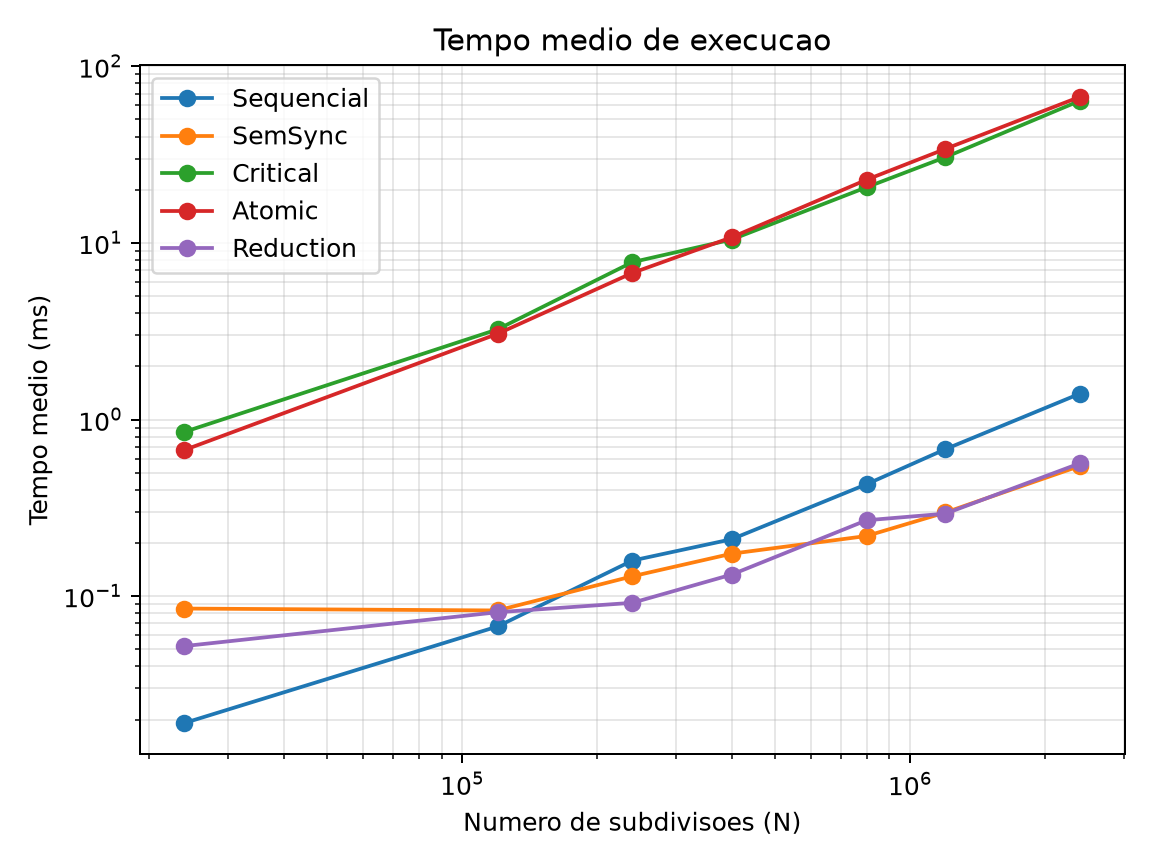
\includegraphics[
        width=0.90\textwidth
    ]{../ATVD6/tempo_medio.png}

    \caption{Tempo médio de execução em função do número de subdivisões.}
    \label{fig:atvd06-tempo}
\end{figure}

A escala logarítmica no eixo dos tempos permite visualizar simultaneamente
implementações com diferenças superiores a uma ordem de grandeza.

\texttt{Critical} e \texttt{Atomic} apresentam crescimento elevado,
enquanto Sequencial e \texttt{Reduction} permanecem em uma região
consideravelmente inferior.


\subsection{Speedup}

\begin{figure}[htbp]
    \centering
    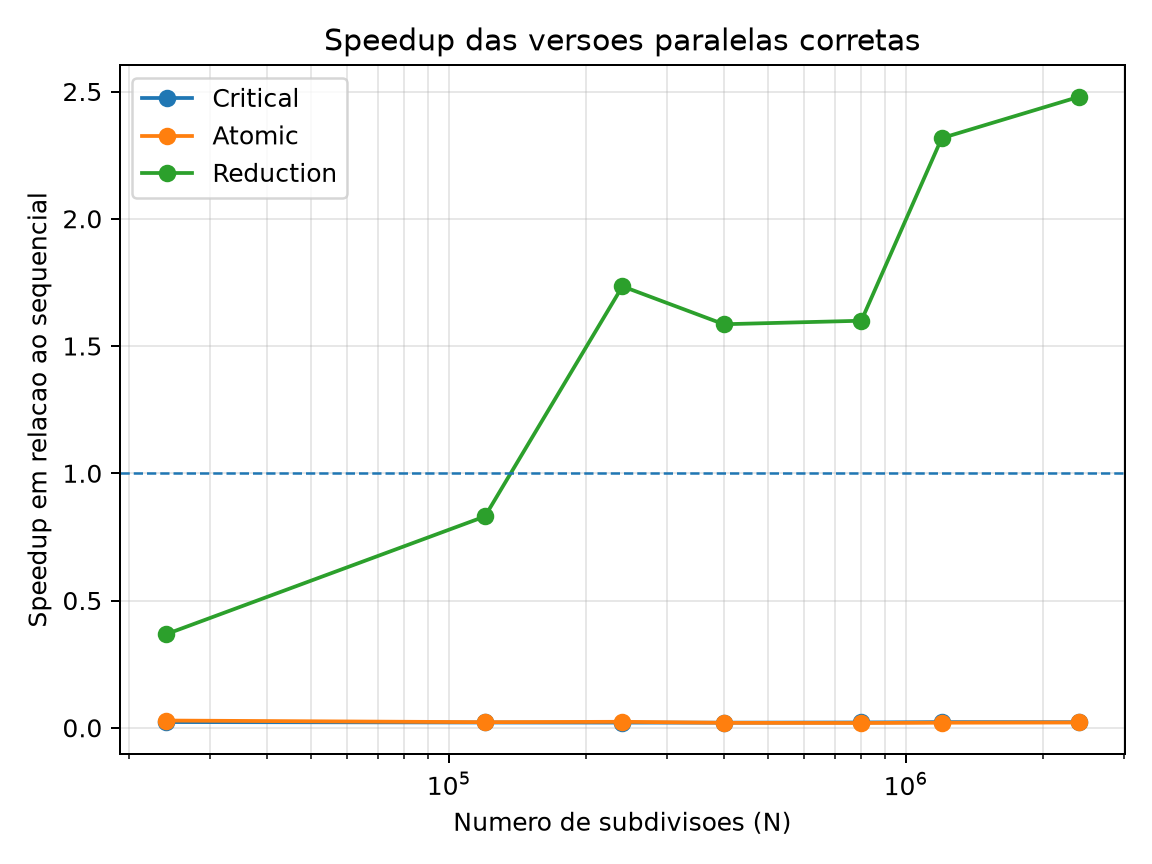
\includegraphics[
        width=0.90\textwidth
    ]{../ATVD6/speedup.png}

    \caption{Speedup das estratégias paralelas funcionalmente válidas.}
    \label{fig:atvd06-speedup}
\end{figure}

A linha \(S=1\) representa o desempenho do baseline sequencial.

\texttt{Critical} e \texttt{Atomic} permanecem abaixo desse limite em todas
as configurações.

\texttt{Reduction} ultrapassa a referência a partir da região entre
\(N=24\,000\) e \(N=120\,000\), tornando o ganho mais evidente nos tamanhos
posteriores.


\subsection{Erro absoluto médio}

\begin{figure}[htbp]
    \centering
    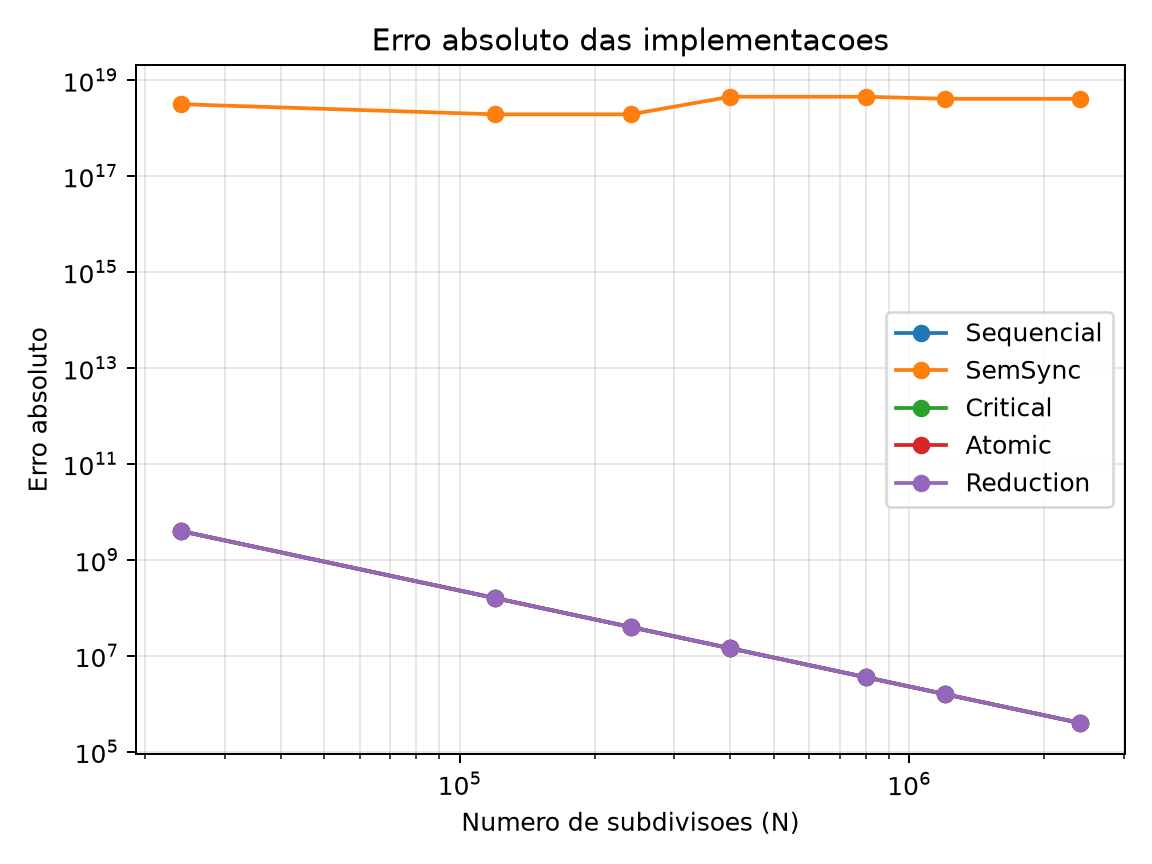
\includegraphics[
        width=0.90\textwidth
    ]{../ATVD6/erro_absoluto.png}

    \caption{Erro absoluto médio das implementações.}
    \label{fig:atvd06-erro}
\end{figure}

Sequencial, \texttt{Critical}, \texttt{Atomic} e \texttt{Reduction}
produzem exatamente os mesmos erros e, portanto, suas curvas se sobrepõem.

A curva de \texttt{SemSync} permanece várias ordens de grandeza acima,
evidenciando o impacto da race condition sobre a correção do resultado.


\section{Análise e discussão}

\label{sec:atvd06-discussao}

\subsection{Impacto da ausência de sincronização}

A versão sem sincronização mostrou diretamente a necessidade de proteger a
operação de redução.

Para \(N=24\,000\), apenas

\begin{equation}
    4/20
\end{equation}

execuções foram corretas.

Para todos os demais valores:

\begin{equation}
    0/20
\end{equation}

resultados foram válidos.

O erro absoluto médio permaneceu na ordem de

\begin{equation}
    10^{18},
\end{equation}

enquanto as versões corretas apresentaram erro determinado apenas pela
discretização do método.

O resultado demonstra que simplesmente distribuir as iterações não é
suficiente: a semântica da atualização compartilhada precisa ser preservada.


\subsection{Desempenho de \texttt{critical}}

A versão \texttt{Critical} garantiu

\begin{equation}
    20/20
\end{equation}

resultados corretos em todas as configurações.

Entretanto, apresentou o maior custo de sincronização.

Para

\begin{equation}
    N=2\,400\,000,
\end{equation}

foram obtidos

\begin{equation}
    T_{\text{seq}}
    =
    1.874432\ \text{ms}
\end{equation}

e

\begin{equation}
    T_{\text{critical}}
    =
    92.877570\ \text{ms}.
\end{equation}

A razão é aproximadamente

\begin{equation}
    \frac{92.877570}{1.874432}
    \approx
    49.5.
\end{equation}

Assim, nessa configuração, a versão \texttt{Critical} foi aproximadamente
\(49.5\) vezes mais lenta que a sequencial.

O speedup correspondente foi

\begin{equation}
    S_{\text{critical}}
    =
    0.020.
\end{equation}

A explicação está na serialização de cada atualização do acumulador. Embora
o cálculo de \(x_i\) e \(f(x_i)\) ocorra em paralelo, todas as threads
precisam entrar repetidamente na mesma região de exclusão mútua.


\subsection{Desempenho de \texttt{atomic}}

A implementação \texttt{Atomic} também produziu resultados corretos em
todas as medições.

Na execução final, foi mais rápida que \texttt{Critical} em todos os valores
de \(N\).

Para

\begin{equation}
    N=2\,400\,000,
\end{equation}

o tempo foi

\begin{equation}
    T_{\text{atomic}}
    =
    61.214450\ \text{ms}.
\end{equation}

Comparando com \texttt{Critical}:

\begin{equation}
    \frac{92.877570}{61.214450}
    \approx
    1.52.
\end{equation}

Apesar dessa melhoria, o speedup em relação ao sequencial foi apenas

\begin{equation}
    S_{\text{atomic}}
    =
    0.031.
\end{equation}

Portanto, \texttt{atomic} reduz o custo em relação a uma região crítica
genérica, mas não elimina o gargalo principal.

Todas as threads ainda executam uma operação de leitura-modificação-escrita
sobre o mesmo acumulador.

Esse padrão produz contenção e tráfego de coerência sobre o mesmo endereço
de memória.


\subsection{Desempenho de \texttt{reduction}}

A implementação utilizando \texttt{reduction} apresentou o melhor
comportamento entre as estratégias paralelas corretas.

Para \(N=24\,000\):

\begin{equation}
    S_{\text{reduction}}
    =
    0.304.
\end{equation}

Portanto, o problema ainda era pequeno demais para compensar o overhead do
OpenMP.

Para \(N=120\,000\):

\begin{equation}
    S_{\text{reduction}}
    =
    1.015,
\end{equation}

indicando desempenho praticamente equivalente ao sequencial.

A partir de \(N=240\,000\), o ganho tornou-se mais evidente:

\begin{equation}
    S_{\text{reduction}}
    =
    1.509.
\end{equation}

Para \(N=400\,000\):

\begin{equation}
    S_{\text{reduction}}
    =
    2.014.
\end{equation}

O maior speedup observado ocorreu para

\begin{equation}
    N=1\,200\,000,
\end{equation}

com

\begin{equation}
    \boxed{
        S_{\text{reduction}}=2.716
    }.
\end{equation}

Com quatro threads, a eficiência correspondente é

\begin{equation}
    E_4
    =
    \frac{2.716}{4}
    \approx
    0.679,
\end{equation}

ou aproximadamente

\begin{equation}
    \boxed{67.9\%}.
\end{equation}


\subsection{Comportamento no maior valor de \(N\)}

Para

\begin{equation}
    N=2\,400\,000,
\end{equation}

o tempo sequencial foi

\begin{equation}
    1.874432\ \text{ms},
\end{equation}

enquanto \texttt{Reduction} apresentou

\begin{equation}
    0.875025\ \text{ms}.
\end{equation}

O speedup foi

\begin{equation}
    S=2.142.
\end{equation}

Esse valor é inferior ao máximo de \(2.716\) observado para
\(N=1\,200\,000\).

O speedup real não precisa crescer monotonicamente com \(N\). Entre os
fatores que podem afetar a relação estão:

\begin{itemize}
    \item escalonamento do sistema operacional;
    \item frequência dinâmica do processador;
    \item estado térmico;
    \item comportamento de cache;
    \item overhead do runtime OpenMP.
\end{itemize}

Mesmo com essa redução no último ponto, a implementação permaneceu mais de
duas vezes mais rápida que o baseline sequencial.


\subsection{Granularidade}

Os resultados demonstram a importância da granularidade.

Para cargas pequenas, o custo de:

\begin{itemize}
    \item iniciar a região paralela;
    \item distribuir iterações;
    \item sincronizar a equipe;
    \item combinar os acumuladores;
\end{itemize}

é comparável ou superior ao trabalho útil.

Isso explica

\begin{equation}
    S<1
\end{equation}

para \texttt{Reduction} em \(N=24\,000\).

À medida que \(N\) cresce, uma quantidade maior de trabalho é distribuída
entre as threads e o overhead fixo é progressivamente amortizado.


\subsection{Correção versus desempenho}

Os resultados também demonstram que desempenho não pode ser avaliado
isoladamente.

Em diversas configurações, \texttt{SemSync} apresenta tempo inferior ao
sequencial. Por exemplo, em \(N=1\,200\,000\), o valor temporal calculado
corresponde a um fator de

\begin{equation}
    2.617
\end{equation}

em relação ao sequencial.

Entretanto:

\begin{equation}
    0/20
\end{equation}

resultados foram corretos.

Portanto, esse valor não pode ser interpretado como speedup de uma solução
válida.

A comparação evidencia a seguinte relação:

\begin{center}
\begin{tabular}{l|c|c}
    \hline
    Estratégia & Correção & Desempenho observado \\
    \hline
    Sequencial & sim & baseline \\
    SemSync & não & não utilizável \\
    Critical & sim & fortemente degradado \\
    Atomic & sim & degradado por contenção \\
    Reduction & sim & melhor estratégia paralela \\
    \hline
\end{tabular}
\end{center}


\subsection{Por que \texttt{reduction} apresenta melhor escalabilidade}

Em \texttt{critical} e \texttt{atomic}, todas as threads atualizam
continuamente a mesma posição de memória.

Em \texttt{reduction}, cada thread mantém sua soma privada durante a maior
parte da execução.

Conceitualmente:

\begin{figure}[htbp]
    \centering
    \begin{tikzpicture}[node distance=0.65cm and 0.65cm, font=\small]
        \node[processo, text width=4.4cm] (iterations)
            {Iterações do laço};
        \node[thread, below left=of iterations, text width=2.7cm] (t1)
            {Thread 1};
        \node[thread, below=of iterations, text width=2.7cm] (t2)
            {Thread 2};
        \node[thread, below right=of iterations, text width=2.7cm] (tp)
            {Thread \(P\)};
        \node[componente, below=of t1, text width=2.7cm] (s1)
            {Soma privada \(S_1\)};
        \node[componente, below=of t2, text width=2.7cm] (s2)
            {Soma privada \(S_2\)};
        \node[componente, below=of tp, text width=2.7cm] (sp)
            {Soma privada \(S_P\)};
        \node[processo, below=1.0cm of s2, text width=3.5cm] (reduction)
            {Redução final};
        \node[componente, below=of reduction, text width=2.7cm] (total)
            {Soma total \(S\)};
        \draw[fluxo] (iterations) -- (t1);
        \draw[fluxo] (iterations) -- (t2);
        \draw[fluxo] (iterations) -- (tp);
        \draw[fluxo] (t1) -- (s1);
        \draw[fluxo] (t2) -- (s2);
        \draw[fluxo] (tp) -- (sp);
        \draw[fluxo] (s1) |- (reduction);
        \draw[fluxo] (s2) -- (reduction);
        \draw[fluxo] (sp) |- (reduction);
        \draw[fluxo] (reduction) -- (total);
    \end{tikzpicture}

    \caption{Estratégia conceitual utilizada pela redução.}
    \label{fig:atvd06-reduction}
\end{figure}

A sincronização deixa de ocorrer em cada iteração e passa a ser concentrada
na combinação final dos resultados parciais.

Essa propriedade explica o desempenho significativamente superior observado
experimentalmente.


\section{Limitações}

\label{sec:atvd06-limitacoes}

O experimento possui algumas limitações que devem ser consideradas na
interpretação dos resultados.

Primeiramente, somente quatro threads foram avaliadas. Portanto, a atividade
permite comparar estratégias de sincronização para uma configuração fixa,
mas não caracteriza a escalabilidade em função do número de threads.

Também foi utilizada apenas a função

\begin{equation}
    f(x)=x^2,
\end{equation}

cujo custo computacional é pequeno e uniforme. Funções mais complexas podem
alterar significativamente a razão entre trabalho útil e overhead de
sincronização.

O uso de \texttt{schedule(static)} é adequado à uniformidade dessa carga,
mas os resultados não caracterizam problemas com custo variável por
iteração.

A aritmética inteira com \texttt{int64\_t} evita erros de ponto flutuante e
facilita a validação. Entretanto, muitas aplicações reais de integração
numérica utilizam \texttt{double}, situação em que a ordem de redução também
pode introduzir pequenas diferenças de arredondamento.

A compilação desabilita a vetorização automática com
\texttt{-fno-tree-vectorize}. Dessa forma, a comparação prioriza os efeitos
de OpenMP e sincronização, não o máximo desempenho disponível com SIMD.

Os atributos \texttt{noinline} e \texttt{noipa} são utilizados para
preservar o trabalho que deve ser medido. Essa decisão é metodologicamente
necessária ao benchmark, mas restringe algumas otimizações que poderiam
ocorrer em um programa de produção.

O batching adaptativo utiliza uma execução piloto para estimar o tamanho do
lote. Flutuações nessa medição podem resultar em lotes cuja duração real
posterior se afasta do alvo de 20 ms. Esse efeito foi especialmente visível
em algumas medições da versão \texttt{SemSync}, cuja execução também é
afetada pela própria condição de corrida.

A versão sem sincronização contém deliberadamente uma race condition.
Consequentemente, seus resultados não são determinísticos e não representam
uma implementação funcionalmente válida.

Por fim, os experimentos foram executados em sistema operacional de
propósito geral. Escalonamento, serviços em segundo plano, frequência
dinâmica e estado térmico podem provocar variações entre execuções.


\section{Conclusões da atividade}

\label{sec:atvd06-conclusao}

A Atividade 6 permitiu avaliar experimentalmente quatro formas distintas de
tratar a dependência sobre o acumulador do método composto do trapézio.

A versão sem sincronização demonstrou diretamente a consequência de uma race
condition. Em \(N=24\,000\), somente quatro das vinte medições produziram o
resultado esperado, enquanto todos os tamanhos posteriores apresentaram
zero resultados válidos em vinte execuções.

A diretiva \texttt{critical} restaurou a correção, porém introduziu forte
serialização. No maior tamanho analisado, essa versão foi aproximadamente
\(49.5\) vezes mais lenta que a execução sequencial.

A diretiva \texttt{atomic} reduziu o custo em relação a
\texttt{critical}, mas continuou apresentando forte contenção sobre o mesmo
acumulador compartilhado. Para \(N=2\,400\,000\), seu speedup foi apenas
\(0.031\).

A versão baseada em \texttt{reduction} apresentou o melhor equilíbrio entre
correção e desempenho. Para problemas pequenos, seu overhead superou o
benefício do paralelismo. Com o crescimento de \(N\), entretanto, o trabalho
paralelo passou a amortizar esse custo.

O maior speedup observado foi

\begin{equation}
    \boxed{2.716}
\end{equation}

com quatro threads em

\begin{equation}
    N=1\,200\,000,
\end{equation}

correspondendo a eficiência aproximada de

\begin{equation}
    \boxed{67.9\%}.
\end{equation}

Os resultados demonstram que a mera introdução de múltiplas threads não
garante ganho de desempenho. A estratégia utilizada para coordenar os dados
compartilhados é determinante.

Para o padrão de soma presente no método do trapézio, a redução mostrou-se
substancialmente mais adequada que a proteção do acumulador em cada
iteração.


\section{Síntese}

\label{sec:atvd06-defesa}

Os principais pontos para defesa oral podem ser sintetizados da seguinte
forma:

\begin{enumerate}

    \item A Atividade 6 implementa experimentalmente a paralelização que havia
    sido discutida teoricamente na Atividade 4.

    \item O problema matemático foi mantido:
    \[
        f(x)=x^2,
        \qquad
        [a,b]=[0,2\,400\,000].
    \]

    \item Foram comparadas cinco versões:
    Sequencial, SemSync, Critical, Atomic e Reduction.

    \item Todas as versões executam exatamente o mesmo cálculo; a principal
    diferença é a forma como o acumulador \texttt{soma} é tratado.

    \item Foram utilizadas quatro threads e
    \texttt{schedule(static)}.

    \item O escalonamento estático foi escolhido porque todas as iterações
    possuem custo aproximadamente uniforme.

    \item Foram realizados três aquecimentos e vinte medições por
    configuração.

    \item Foi utilizado batching adaptativo com alvo de aproximadamente
    20 ms, porque uma quantidade fixa de repetições seria inadequada para
    versões com custos muito diferentes.

    \item O tempo apresentado corresponde à média das vinte medições,
    conforme solicitado pelo enunciado.

    \item A versão SemSync possui uma race condition no acumulador.

    \item Em \(N=24\,000\), SemSync produziu apenas 4 resultados corretos em
    20 medições; para todos os demais valores, produziu 0/20.

    \item O erro de SemSync é apresentado como erro absoluto médio das vinte
    medições, e não como erro de uma única execução.

    \item Critical resolve a race condition, mas serializa cada atualização
    da soma.

    \item No maior caso, Critical demorou aproximadamente 92.88 ms contra
    1.87 ms do sequencial, sendo cerca de 49.5 vezes mais lento.

    \item Atomic também garante correção e foi mais rápido que Critical na
    execução final, porém todas as threads continuam disputando o mesmo
    acumulador.

    \item No maior caso, Atomic apresentou speedup de apenas
    \[
        0.031.
    \]

    \item Reduction utiliza acumuladores privados e combina os resultados ao
    final, evitando sincronização sobre a soma em cada iteração.

    \item Para \(N=24\,000\), Reduction ainda foi mais lenta que o
    sequencial:
    \[
        S=0.304.
    \]

    \item Em \(N=120\,000\), o desempenho ficou praticamente no ponto de
    equilíbrio:
    \[
        S=1.015.
    \]

    \item A partir dos tamanhos seguintes, Reduction passou a apresentar
    ganho consistente.

    \item O maior speedup observado foi
    \[
        S=2.716
    \]
    para
    \[
        N=1\,200\,000.
    \]

    \item Com quatro threads, isso corresponde a eficiência de
    aproximadamente
    \[
        67.9\%.
    \]

    \item O speedup não cresceu monotonicamente: em
    \(N=2\,400\,000\), Reduction apresentou
    \[
        S=2.142.
    \]
    Essa variação é compatível com fatores reais de execução como runtime
    OpenMP, escalonamento, frequência dinâmica e estado do sistema.

    \item O aparente speedup da versão SemSync não deve ser interpretado como
    ganho válido, pois desempenho sem correção funcional não representa uma
    solução utilizável.

    \item A principal conclusão é que, para uma soma paralela, proteger cada
    atualização com Critical ou Atomic pode introduzir contenção suficiente
    para tornar o programa muito mais lento.

    \item Para esse padrão computacional, Reduction foi a estratégia que
    melhor preservou simultaneamente correção e desempenho.

\end{enumerate}

\chapter{Atividade 7 -- Escopo de variáveis e estratégias de escalonamento em OpenMP}
\label{chap:atvd07}


% ============================================================
\section{Enunciado da tarefa}
\label{sec:atvd07-enunciado}

\begin{quote}
Implemente diferentes versões de um programa para calcular quantos números
primos existem entre 2 e um valor máximo \(n\). O programa deve ser
paralelizado utilizando OpenMP.

Devem ser implementadas versões com a variável do contador utilizando apenas
\texttt{private}, apenas \texttt{firstprivate}, apenas
\texttt{lastprivate}, \texttt{firstprivate} e \texttt{lastprivate},
uso de \texttt{default(none)} e uma versão paralela utilizando
\texttt{reduction}.

A partir da versão selecionada como a de melhor comportamento, implemente
versões considerando os escalonadores \texttt{static}, \texttt{dynamic},
\texttt{guided}, \texttt{auto} e \texttt{runtime}. Analise os tempos médios
de execução de cada versão à medida que \(n\) aumenta e utilize gráficos
para apresentar e analisar os resultados.
\end{quote}


% ============================================================
\section{Objetivos e requisitos}
\label{sec:atvd07-objetivos}

A atividade teve como objetivo aprofundar dois aspectos fundamentais da
programação paralela com OpenMP: o escopo de variáveis em regiões paralelas
e a distribuição das iterações de um laço entre as threads.

O problema computacional foi mantido em continuidade com a Atividade 5:
determinar a quantidade de números primos existentes no intervalo

\[
[2,n].
\]

Essa continuidade permitiu reutilizar uma implementação previamente
validada e concentrar o experimento nos novos mecanismos do OpenMP.

Os objetivos específicos foram:

\begin{itemize}
    \item reutilizar o algoritmo de contagem de primos desenvolvido na
    Atividade 5;

    \item preservar a mesma função de teste de primalidade em todas as
    versões;

    \item analisar o comportamento das cláusulas
    \texttt{private},
    \texttt{firstprivate},
    \texttt{lastprivate},
    \texttt{firstprivate + lastprivate},
    \texttt{default(none)} e
    \texttt{reduction};

    \item verificar quais dessas construções preservam a contagem global
    correta;

    \item selecionar uma implementação paralela funcionalmente correta para
    o experimento de escalonamento;

    \item comparar as políticas
    \texttt{static},
    \texttt{dynamic},
    \texttt{guided},
    \texttt{auto} e
    \texttt{runtime};

    \item medir o tempo médio de execução das diferentes versões;

    \item manter fixos os demais parâmetros experimentais para isolar o
    efeito das cláusulas estudadas;

    \item representar os resultados por meio de tabelas e gráficos;

    \item discutir correção, sincronização, overhead e balanceamento de
    carga.
\end{itemize}

A atividade foi estruturada em dois experimentos principais:

\begin{enumerate}
    \item comparação das cláusulas de escopo de dados;
    \item comparação das estratégias de escalonamento utilizando
    \texttt{reduction}.
\end{enumerate}


% ============================================================
\section{Fundamentação conceitual}
\label{sec:atvd07-fundamentacao}

\subsection{Paralelismo na contagem de números primos}

A contagem considera todos os candidatos pertencentes ao intervalo

\[
2,3,\ldots,n.
\]

Para cada candidato \(x\), é realizada uma classificação independente:

\[
P(x)=
\begin{cases}
1, & \text{se } x \text{ é primo},\\
0, & \text{caso contrário}.
\end{cases}
\]

A quantidade total de números primos é, portanto,

\[
C(n)=\sum_{x=2}^{n}P(x).
\]

Como a classificação de um candidato não depende dos demais, o laço que
percorre os candidatos apresenta paralelismo de dados natural.

O desafio está na agregação das contribuições individuais para o contador
global.


\subsection{Variáveis compartilhadas e privadas}

Em uma região paralela OpenMP, as threads podem acessar variáveis com
diferentes regras de compartilhamento.

Uma variável compartilhada possui uma única instância visível pelas
threads, enquanto uma variável privada possui uma instância independente
para cada thread.

Essa distinção é fundamental para a contagem de primos. Embora o trabalho
de testar os candidatos seja independente, a contagem final representa uma
operação global:

\[
C=C_0+C_1+\cdots+C_{T-1},
\]

onde \(C_i\) representa a quantidade encontrada pela thread \(i\).

A simples criação de cópias privadas não realiza automaticamente essa soma.


\subsection{\texttt{private}}

A cláusula

\begin{verbatim}
private(count)
\end{verbatim}

cria uma cópia independente de \texttt{count} para cada thread.

As cópias por thread são representadas na Figura~\ref{fig:atvd07-private}.

\begin{figure}[htbp]
    \centering
    \begin{tikzpicture}[node distance=0.6cm and 0.45cm, font=\small]
        \node[componente, text width=3.4cm] (shared)
            {Variável externa\\\texttt{count}};
        \node[processo, right=1.1cm of shared, text width=3.5cm] (clause)
            {\texttt{private(count)}};
        \node[thread, below left=of clause, text width=2.4cm] (t0)
            {Thread 0\\cópia privada};
        \node[thread, below=of clause, text width=2.4cm] (t1)
            {Thread 1\\cópia privada};
        \node[thread, below right=of clause, text width=2.4cm] (t2)
            {Thread \(T-1\)\\cópia privada};
        \node[componente, below=0.9cm of t1, text width=4.2cm] (discard)
            {Cópias descartadas\\sem soma global};
        \draw[fluxo] (shared) -- (clause);
        \draw[fluxo] (clause) -- (t0);
        \draw[fluxo] (clause) -- (t1);
        \draw[fluxo] (clause) -- (t2);
        \draw[fluxo] (t0) |- (discard);
        \draw[fluxo] (t1) -- (discard);
        \draw[fluxo] (t2) |- (discard);
    \end{tikzpicture}
    \caption{Cópias privadas independentes sem agregação ao contador externo.}
    \label{fig:atvd07-private}
\end{figure}

As cópias privadas não recebem automaticamente o valor anteriormente
armazenado na variável original e também não são automaticamente combinadas
ao término da região paralela.

Assim,

\[
\texttt{private}
\]

resolve o isolamento entre as threads, mas não resolve a agregação das
contagens.


\subsection{\texttt{firstprivate}}

A cláusula

\begin{verbatim}
firstprivate(count)
\end{verbatim}

também cria uma cópia privada para cada thread, mas inicializa essa cópia
com o valor existente antes da região paralela.

Se inicialmente

\[
count=0,
\]

então todas as threads começam com

\[
count_i=0.
\]

Ao final da região, entretanto, essas cópias continuam sendo descartadas.

Portanto,

\[
\texttt{firstprivate}
\]

resolve a inicialização das cópias, mas não implementa uma operação de
redução.


\subsection{\texttt{lastprivate}}

A cláusula

\begin{verbatim}
lastprivate(count)
\end{verbatim}

torna a variável privada durante o laço e, ao término da região paralela,
transfere para a variável externa o valor correspondente à última iteração
lógica do laço.

Isso não representa a soma das contribuições das threads.

Formalmente,

\[
\texttt{lastprivate}
\neq
\sum_i C_i.
\]

Existe ainda um cuidado importante: a cópia privada criada por
\texttt{lastprivate} não deve ser lida sem inicialização.

Na implementação desta atividade, \texttt{count} é explicitamente definido
antes de ser utilizado em cada iteração, evitando leitura de valor
indeterminado.


\subsection{\texttt{firstprivate} e \texttt{lastprivate}}

A combinação

\begin{verbatim}
firstprivate(count) lastprivate(count)
\end{verbatim}

faz com que cada cópia privada seja inicializada com o valor externo e que,
ao final, a cópia associada à última iteração lógica seja propagada para a
variável externa.

Entretanto, continua não existindo uma agregação global.

Assim,

\[
\boxed{
\texttt{firstprivate + lastprivate}
\neq
\texttt{reduction}
}
\]


\subsection{\texttt{default(none)}}

A cláusula

\begin{verbatim}
default(none)
\end{verbatim}

obriga que o programador declare explicitamente a classificação das
variáveis utilizadas na região paralela.

Seu objetivo é aumentar a clareza da política de compartilhamento e reduzir
erros decorrentes de classificações implícitas.

Entretanto,

\[
\boxed{
\texttt{default(none)}
\text{ não é um mecanismo de sincronização}
}
\]

Se uma variável for explicitamente declarada como compartilhada e múltiplas
threads realizarem atualizações concorrentes sem proteção, a condição de
corrida continua existindo.


\subsection{Condição de corrida}

A operação

\begin{verbatim}
++count;
\end{verbatim}

não deve ser interpretada como uma única operação indivisível.

Conceitualmente, ela envolve:

\begin{enumerate}
    \item leitura do valor;
    \item incremento;
    \item escrita do novo valor.
\end{enumerate}

Se duas ou mais threads realizarem essas operações simultaneamente sobre o
mesmo contador compartilhado, atualizações podem ser perdidas.

Essa situação constitui uma \textit{data race}.

Os resultados produzidos por uma implementação com condição de corrida não
possuem garantia de correção e uma eventual coincidência com o resultado
esperado não elimina o erro de sincronização.


\subsection{\texttt{reduction}}

O padrão matemático da contagem de primos é uma soma de resultados
parciais.

OpenMP fornece diretamente esse padrão por meio de:

\begin{verbatim}
reduction(+:count)
\end{verbatim}

Cada thread realiza sua própria acumulação e, ao final da região, OpenMP
combina os valores privados.

O processo de combinação é ilustrado na Figura~\ref{fig:atvd07-reduction}.

\begin{figure}[htbp]
    \centering
    \begin{tikzpicture}[node distance=0.55cm and 0.55cm, font=\small]
        \node[thread, text width=2.4cm] (t0) {Thread 0\\soma privada \(C_0\)};
        \node[thread, right=of t0, text width=2.4cm] (t1) {Thread 1\\soma privada \(C_1\)};
        \node[thread, right=of t1, text width=2.4cm] (tt) {Thread \(T-1\)\\soma privada \(C_{T-1}\)};
        \node[processo, below=of t1, text width=4.0cm] (combine)
            {Combinar\\\texttt{reduction(+:count)}};
        \node[componente, below=of combine, text width=3.2cm] (total)
            {Contagem global\\\(C=\sum_i C_i\)};
        \draw[fluxo] (t0) -- (combine);
        \draw[fluxo] (t1) -- (combine);
        \draw[fluxo] (tt) -- (combine);
        \draw[fluxo] (combine) -- (total);
    \end{tikzpicture}
    \caption{Agregação das contagens privadas pela cláusula \texttt{reduction}.}
    \label{fig:atvd07-reduction}
\end{figure}

Assim,

\[
C=\sum_{i=0}^{T-1}C_i.
\]

A cláusula representa diretamente a operação necessária para obter a
contagem global.


\subsection{Escalonamento de iterações}

Depois de definida uma implementação paralela correta, é necessário decidir
como as iterações do laço serão distribuídas entre as threads.

Em OpenMP essa política pode ser especificada por meio da cláusula
\texttt{schedule}.


\subsubsection{\texttt{static}}

Na política

\begin{verbatim}
schedule(static)
\end{verbatim}

as iterações são distribuídas previamente entre as threads.

Essa abordagem possui baixo overhead e comportamento previsvisível.

Entretanto, uma quantidade semelhante de iterações não implica
necessariamente uma quantidade semelhante de trabalho.


\subsubsection{\texttt{dynamic}}

Na política

\begin{verbatim}
schedule(dynamic)
\end{verbatim}

novos blocos de iterações são obtidos pelas threads à medida que o trabalho
anterior é concluído.

Isso pode melhorar o balanceamento de cargas irregulares, mas aumenta o
custo de gerenciamento do escalonamento.


\subsubsection{\texttt{guided}}

Em

\begin{verbatim}
schedule(guided)
\end{verbatim}

o trabalho também é distribuído dinamicamente, mas blocos maiores são
utilizados inicialmente e seu tamanho é progressivamente reduzido.

A estratégia busca combinar:

\[
\text{baixo overhead inicial}
\]

com

\[
\text{melhor balanceamento próximo ao final}.
\]


\subsubsection{\texttt{auto}}

Com

\begin{verbatim}
schedule(auto)
\end{verbatim}

a escolha da forma de distribuição é delegada à implementação OpenMP.

O programa não determina explicitamente qual estratégia interna será
utilizada.


\subsubsection{\texttt{runtime}}

Com

\begin{verbatim}
schedule(runtime)
\end{verbatim}

a configuração do escalonamento é determinada em tempo de execução.

Nesta atividade, a política foi explicitamente configurada como

\[
\texttt{dynamic},\quad chunk=1.
\]

Dessa forma, o significado de \texttt{runtime} permaneceu reproduzível
durante o experimento.


\subsection{Irregularidade da carga}

O custo do teste de primalidade não é uniforme.

Números pares são rejeitados imediatamente, enquanto candidatos ímpares,
especialmente números primos maiores, podem exigir vários testes de
divisibilidade.

Assim,

\[
W(i)\neq W(j),
\]

onde \(W(x)\) representa o trabalho necessário para testar o candidato
\(x\).

Essa característica torna o problema apropriado para avaliar políticas de
escalonamento.


\subsection{Tempo médio}

O enunciado solicita a análise do tempo médio de execução.

Para \(M=20\) medições,

\[
T_{\mathrm{medio}}
=
\frac{1}{20}
\sum_{i=1}^{20}T_i.
\]

Essa estatística foi utilizada como medida principal nesta atividade.


% ============================================================
\section{Interpretação didática da tarefa}
\label{sec:atvd07-interpretacao}

A atividade foi interpretada como uma continuação direta do estudo iniciado
na Atividade 5.

Na atividade anterior, verificou-se que uma simples paralelização do laço
com um contador compartilhado produzia uma condição de corrida e que a
cláusula \texttt{reduction} fornecia a agregação correta.

Nesta atividade, o objetivo foi decompor esse problema em duas questões.

A primeira foi:

\begin{quote}
Como diferentes cláusulas de escopo alteram o comportamento de uma variável
utilizada como contador?
\end{quote}

A segunda foi:

\begin{quote}
Depois de obtida uma implementação correta, como a política utilizada para
distribuir as iterações influencia o desempenho?
\end{quote}

Assim, a progressão didática adotada está representada na
Figura~\ref{fig:atvd07-percurso}.

\begin{figure}[htbp]
    \centering
    \begin{tikzpicture}[node distance=0.45cm and 0.45cm, font=\small]
        \node[processo, text width=4.4cm] (seq) {Contagem sequencial};
        \node[componente, below=of seq, text width=4.4cm] (scope)
            {Investigar escopo de dados};
        \node[thread, below left=of scope, text width=2.7cm] (private)
            {\texttt{private}, \texttt{firstprivate},\\\texttt{lastprivate} e combinação};
        \node[thread, below=of scope, text width=2.7cm] (default)
            {\texttt{default(none)}};
        \node[thread, below right=of scope, text width=2.7cm] (reduction)
            {\texttt{reduction}};
        \node[componente, below=0.8cm of default, text width=3.8cm] (check)
            {Validar resultados};
        \node[decisao, below=of check, text width=3.2cm] (valid)
            {Contagem correta?};
        \node[componente, right=1.2cm of valid, yshift=-0.7cm, text width=2.5cm] (discard)
            {Descartar versão incorreta};
        \node[processo, below=of valid, text width=4.4cm] (selected)
            {Selecionar \texttt{reduction}};
        \node[componente, below=of selected, text width=4.4cm] (schedule)
            {Comparar schedules\\static, dynamic, guided, auto, runtime};
        \node[processo, below=of schedule, text width=4.4cm] (performance)
            {Analisar desempenho};
        \draw[fluxo] (seq) -- (scope);
        \draw[fluxo] (scope) -- (private);
        \draw[fluxo] (scope) -- (default);
        \draw[fluxo] (scope) -- (reduction);
        \draw[fluxo] (private.south) |- (check.west);
        \draw[fluxo] (default.south) -- (check.north);
        \draw[fluxo] (reduction.south) |- (check.east);
        \draw[fluxo] (check) -- (valid);
        \draw[fluxo] (valid) -- node[right] {sim} (selected);
        \draw[fluxo] (valid.east) -- node[pos=0.5,above] {não} (discard.west);
        \draw[fluxo] (selected) -- (schedule);
        \draw[fluxo] (schedule) -- (performance);
    \end{tikzpicture}
    \caption{Progressão da análise de escopo até a comparação de desempenho.}
    \label{fig:atvd07-percurso}
\end{figure}

A atividade, portanto, separa explicitamente dois problemas que podem ser
confundidos em uma primeira abordagem à programação paralela:

\[
\boxed{\text{compartilhamento de dados}}
\]

e

\[
\boxed{\text{distribuição do trabalho}}.
\]


% ============================================================
\section{Modelagem da solução}
\label{sec:atvd07-modelagem}

\subsection{Estrutura geral}

A solução foi implementada por adaptação direta do programa desenvolvido na
Atividade 5.

Foram preservados:

\begin{itemize}
    \item o algoritmo de primalidade;
    \item os valores de \(N\);
    \item as contagens conhecidas de primos;
    \item a temporização baseada em \texttt{omp\_get\_wtime()};
    \item os aquecimentos;
    \item as repetições internas calibradas;
    \item a validação funcional;
    \item o uso de quatro threads.
\end{itemize}

A nova implementação foi dividida em dois experimentos.


\subsubsection{Experimento A -- Escopo de dados}

Foram consideradas sete implementações:

\begin{enumerate}
    \item sequencial;
    \item \texttt{private};
    \item \texttt{firstprivate};
    \item \texttt{lastprivate};
    \item \texttt{firstprivate + lastprivate};
    \item \texttt{default(none)};
    \item \texttt{reduction}.
\end{enumerate}

A versão sequencial foi utilizada como referência.

A seleção da implementação a ser utilizada posteriormente não foi baseada
apenas no menor tempo, mas na ordem:

\[
\boxed{
\text{correção}
\longrightarrow
\text{desempenho}
}
\]


\subsubsection{Experimento B -- Escalonamento}

A versão com \texttt{reduction}, validada no primeiro experimento, foi
utilizada como base.

A única dimensão modificada passou a ser a política de escalonamento:

\begin{enumerate}
    \item \texttt{static};
    \item \texttt{dynamic};
    \item \texttt{guided};
    \item \texttt{auto};
    \item \texttt{runtime}.
\end{enumerate}

Todas as versões continuaram utilizando exatamente o mesmo teste de
primalidade e a mesma redução.


\subsection{Principais funções e componentes}

A organização principal do programa é apresentada na
Tabela~\ref{tab:atvd07-componentes}.

\begin{table}[htbp]
\centering
\caption{Principais componentes da implementação da Atividade 7.}
\label{tab:atvd07-componentes}
\small
\begin{tabular}{|p{0.38\textwidth}|p{0.52\textwidth}|}
\hline
\textbf{Componente} & \textbf{Responsabilidade} \\
\hline
\texttt{is\_prime()} &
Teste de primalidade comum a todas as versões. \\
\hline

\texttt{count\_primes\_sequential()} &
Implementação sequencial de referência. \\
\hline

\texttt{count\_primes\_private()} &
Versão com cópias privadas do contador. \\
\hline

\texttt{count\_primes\_firstprivate()} &
Versão cujas cópias privadas recebem o valor inicial do contador. \\
\hline

\texttt{count\_primes\_lastprivate()} &
Versão que propaga o valor da última iteração lógica. \\
\hline

\texttt{count\_primes\_first\_lastprivate()} &
Combina inicialização privada e propagação da última iteração. \\
\hline

\texttt{count\_primes\_default\_none()} &
Declara explicitamente o compartilhamento, mantendo o contador
compartilhado sem sincronização. \\
\hline

\texttt{count\_primes\_reduction()} &
Implementação correta com redução e \texttt{schedule(static)}. \\
\hline

Funções de \texttt{schedule} &
Implementam \texttt{dynamic}, \texttt{guided}, \texttt{auto} e
\texttt{runtime}, sempre com redução. \\
\hline

\texttt{run\_timed\_batch()} &
Executa várias chamadas dentro de um único intervalo cronometrado. \\
\hline

\texttt{calibrate\_internal\_repetitions()} &
Determina um número comum de repetições internas por valor de \(N\). \\
\hline

\texttt{run\_warmups\_rotated()} &
Executa aquecimentos alterando a ordem inicial das versões. \\
\hline

\texttt{benchmark\_function\_set()} &
Executa vinte medições por versão, com ordem rotacionada, e calcula a
média. \\
\hline

Funções de exportação CSV &
Persistem os resultados utilizados na geração e análise dos gráficos. \\
\hline
\end{tabular}
\end{table}


% ============================================================
\section{Decisões de projeto e trade-offs}
\label{sec:atvd07-decisoes}

\subsection{Reutilização da Atividade 5}

A implementação não foi reconstruída do início.

O código anterior já fornecia:

\begin{itemize}
    \item teste de primalidade validado;
    \item valores conhecidos de referência;
    \item controle da quantidade de threads;
    \item temporização;
    \item aquecimentos;
    \item calibração de lotes;
    \item mecanismo para impedir a eliminação da computação pelo compilador.
\end{itemize}

A reutilização reduz a quantidade de novas variáveis introduzidas no
experimento e mantém continuidade entre as atividades.


\subsection{Mesma função de primalidade}

Todas as versões utilizam a mesma função \texttt{is\_prime()}.

Não foram introduzidos algoritmos alternativos, como crivos ou novas
otimizações específicas.

Assim, as diferenças observadas decorrem das construções OpenMP avaliadas e
não de algoritmos diferentes.


\subsection{Tratamento seguro de \texttt{private}}

Uma variável criada com \texttt{private} não herda automaticamente o valor
da variável externa.

Utilizar diretamente

\begin{verbatim}
++count;
\end{verbatim}

sem inicialização produziria leitura de um valor indeterminado.

Por isso, a implementação inicializa explicitamente a cópia privada de cada
thread:

\begin{verbatim}
count = 0;
\end{verbatim}

As contagens privadas são armazenadas temporariamente apenas para manter o
trabalho computacional observável durante a otimização do compilador.

O contador externo permanece zero.


\subsection{Observabilidade das cópias privadas}

Nas versões \texttt{private} e \texttt{firstprivate}, o resultado das cópias
privadas seria descartado ao final da região.

Isso poderia permitir ao compilador identificar parte da computação como
sem efeito observável.

Por esse motivo, as contagens parciais são utilizadas na formação de uma
assinatura consumida pelo programa.

Essa estratégia preserva o significado do experimento, mas adiciona uma
pequena quantidade de trabalho auxiliar às versões correspondentes.

Consequentemente, seus tempos devem ser interpretados como os tempos das
implementações experimentais efetivamente utilizadas, e não como uma
medida isolada do custo da cláusula OpenMP.


\subsection{Tratamento seguro de \texttt{lastprivate}}

A cópia associada a \texttt{lastprivate} não deve ser incrementada a partir
de um valor não inicializado.

Para evitar comportamento indefinido, cada iteração atribui

\begin{verbatim}
count = 0;
\end{verbatim}

antes de testar o candidato.

O valor final passa, portanto, a representar a classificação da última
iteração lógica.

Como todos os valores de \(N\) utilizados são pares, a última iteração
corresponde a um número não primo e o resultado observado foi zero em todos
os casos.


\subsection{Separação entre \texttt{default(none)} e \texttt{reduction}}

A versão com \texttt{default(none)} foi mantida separada da versão com
\texttt{reduction}.

O contador foi explicitamente declarado como compartilhado:

\begin{verbatim}
default(none) shared(n, count)
\end{verbatim}

mas não recebeu proteção adicional.

Essa decisão permite demonstrar que declarar explicitamente o escopo das
variáveis não elimina uma condição de corrida.


\subsection{Correção antes de desempenho}

Versões funcionalmente incorretas também foram cronometradas para observar
seu comportamento experimental.

Entretanto, elas não foram consideradas candidatas à melhor solução.

O critério utilizado está representado na Figura~\ref{fig:atvd07-correcao}.

\begin{figure}[htbp]
    \centering
    \begin{tikzpicture}[node distance=0.75cm and 1.0cm, font=\small]
        \node[decisao, text width=3.2cm] (valid)
            {Resultado correto?};
        \node[componente, below left=of valid, text width=3.4cm] (discard)
            {Descartar como\\solução paralela};
        \node[processo, below right=of valid, text width=3.4cm] (perf)
            {Comparar desempenho};
        \draw[fluxo] (valid) -| node[pos=0.25,left] {não} (discard);
        \draw[fluxo] (valid) -| node[pos=0.25,right] {sim} (perf);
    \end{tikzpicture}
    \caption{A correção funcional precede a comparação de desempenho.}
    \label{fig:atvd07-correcao}
\end{figure}

Essa decisão evita interpretar uma implementação que realiza uma computação
incorreta como uma otimização válida.


\subsection{Seleção de \texttt{reduction}}

A versão com redução foi a única versão paralela do primeiro experimento que
reproduziu a contagem global correta para todos os valores de \(N\).

Ela foi, portanto, escolhida como base do experimento de escalonamento.


\subsection{Número fixo de threads}

Foram utilizadas quatro threads em todas as execuções.

A quantidade de threads não foi variada porque o objetivo da atividade era
isolar:

\begin{enumerate}
    \item o efeito do escopo das variáveis;
    \item o efeito do escalonamento.
\end{enumerate}

Adicionar diferentes quantidades de threads introduziria uma terceira
dimensão experimental.


\subsection{Não variação explícita do tamanho dos blocos}

Não foi realizado um experimento separado de \textit{chunk size}.

A comparação foi mantida concentrada nas políticas solicitadas no
enunciado.

No caso de \texttt{runtime}, foi utilizada explicitamente a configuração

\[
\texttt{dynamic,1}.
\]


\subsection{Média em vez de mediana}

Na Atividade 5 foi utilizada a mediana.

Nesta atividade, entretanto, o enunciado solicita tempos médios de
execução.

Assim, a estatística principal foi alterada para a média aritmética das
vinte medições:

\[
\bar{T}
=
\frac{1}{20}
\sum_{i=1}^{20}T_i.
\]


\subsection{Rotação da ordem de execução}

Com várias versões no mesmo experimento, executar sempre as funções na mesma
ordem poderia introduzir viés sistemático.

Foi implementada uma rotação determinística.

O mecanismo de rotação está representado na
Figura~\ref{fig:atvd07-rotacao}.

\begin{figure}[htbp]
    \centering
    \begin{tikzpicture}[node distance=0.55cm and 0.55cm, font=\small]
        \node[processo, text width=2.8cm] (measurement)
            {Medição \(m\)};
        \node[componente, right=of measurement, text width=3.4cm] (start)
            {Escolher início\\\(m \bmod K\)};
        \node[componente, right=of start, text width=4.0cm] (run)
            {Executar \(K\) versões\\em ordem circular};
        \node[processo, right=of run, text width=2.8cm] (next)
            {Próxima medição\\\(m \leftarrow m+1\)};
        \draw[fluxo] (measurement) -- (start);
        \draw[fluxo] (start) -- (run);
        \draw[fluxo] (run) -- (next);
        \draw[fluxo] (next.north) -- ++(0,0.65) -| (start.north);
    \end{tikzpicture}
    \caption{Rotação determinística da ordem das versões entre medições.}
    \label{fig:atvd07-rotacao}
\end{figure}

A mesma estratégia foi utilizada durante os aquecimentos.


\subsection{Repetições internas comuns}

O número de repetições internas foi calibrado para cada \(N\) utilizando a
implementação sequencial e a implementação de referência com
\texttt{reduction} e \texttt{static}.

O mesmo número de repetições foi então utilizado para as demais versões
daquele \(N\).

Essa abordagem preserva comparabilidade entre as configurações.

Como consequência, uma versão posteriormente mais rápida que a utilizada na
calibração pode gerar um lote menor que o alvo nominal de \(100\,\mathrm{ms}\).
O limite deve, portanto, ser entendido como um alvo da calibração da
referência, e não como garantia para todas as variantes.


% ============================================================
\section{Representação estrutural da implementação}
\label{sec:atvd07-estrutura}

A estrutura geral do programa pode ser representada pelo diagrama a seguir.

\begin{figure}[htbp]
    \centering
    \resizebox{0.88\textwidth}{!}{%
    \begin{tikzpicture}[node distance=0.45cm, font=\small]
        \node[processo, text width=3.0cm] (main) {\texttt{main()}};
        \node[componente, below=of main, text width=6.6cm] (setup)
            {Configuração comum\\4 threads, entrada \(N\), \texttt{is\_prime()}};
        \node[thread, below=of setup, text width=7.6cm] (scope)
            {Experimento A -- escopo de dados\\
             Sequencial, \texttt{private}, \texttt{firstprivate},
             \texttt{lastprivate}, combinação, \texttt{default(none)}
             e \texttt{reduction}};
        \node[processo, below=of scope, text width=6.6cm] (select)
            {Validar resultados e selecionar \texttt{reduction}};
        \node[thread, below=of select, text width=7.6cm] (schedule)
            {Experimento B -- escalonamento\\
             \texttt{reduction} com \texttt{static}, \texttt{dynamic},
             \texttt{guided}, \texttt{auto} e \texttt{runtime}};
        \node[processo, below=of schedule, text width=6.6cm] (benchmark)
            {\texttt{benchmark\_function\_set()}\\
             calibração, aquecimentos e 20 medições};
        \node[componente, below=of benchmark, text width=7.0cm] (outputs)
            {Exportar \texttt{data\_sharing\_results.csv}\\
             e \texttt{scheduling\_results.csv}};

        \draw[fluxo] (main) -- (setup);
        \draw[fluxo] (setup) -- (scope);
        \draw[fluxo] (scope) -- (select);
        \draw[fluxo] (select) -- (schedule);
        \draw[fluxo] (schedule) -- (benchmark);
        \draw[fluxo] (benchmark) -- (outputs);
    \end{tikzpicture}%
    }
    \caption{Diagrama UML de componentes dos dois experimentos da Atividade 7.}
    \label{fig:atvd07-estrutura}
\end{figure}


% ============================================================
\section{Fluxo de execução}
\label{sec:atvd07-fluxo}

O fluxo completo da execução está modelado na
Figura~\ref{fig:atvd07-fluxo}.

\begin{figure}[htbp]
    \centering
    \resizebox{!}{0.70\textheight}{%
    \begin{tikzpicture}[node distance=0.45cm, font=\small]
        \node[processo, text width=5.8cm] (start) {Início};
        \node[componente, below=of start, text width=6.8cm] (setup)
            {Configurar 4 threads, desativar ajuste dinâmico\\
             e definir \texttt{runtime = dynamic, chunk=1}};
        \node[componente, below=of setup, text width=6.8cm] (validate)
            {Validar \texttt{is\_prime()} e confirmar a equipe de threads};
        \node[thread, below=of validate, text width=7.2cm] (experimentA)
            {Experimento A: para cada \(N\), executar as sete versões de
             escopo, validar a referência, calibrar repetições, realizar
             3 aquecimentos e 20 medições rotacionadas; calcular médias};
        \node[decisao, below=of experimentA, text width=3.6cm] (select)
            {Reduction reproduz a referência?};
        \node[processo, right=1.0cm of select, text width=2.7cm] (abort)
            {Interromper};
        \node[thread, below=of select, text width=7.2cm] (experimentB)
            {Experimento B: para cada \(N\), executar reduction com os cinco
             schedules, validar contagens, aquecer e realizar 20 medições
             rotacionadas; calcular médias};
        \node[componente, below=of experimentB, text width=6.8cm] (export)
            {Imprimir tabelas e exportar os dois arquivos CSV};
        \node[processo, below=of export, text width=5.8cm] (end) {Fim};

        \draw[fluxo] (start) -- (setup);
        \draw[fluxo] (setup) -- (validate);
        \draw[fluxo] (validate) -- (experimentA);
        \draw[fluxo] (experimentA) -- (select);
        \draw[fluxo] (select.east) -- node[above] {não} (abort.west);
        \draw[fluxo] (select) -- node[right] {sim} (experimentB);
        \draw[fluxo] (experimentB) -- (export);
        \draw[fluxo] (export) -- (end);
    \end{tikzpicture}%
    }
    \caption{Diagrama UML de atividade do fluxo dos experimentos A e B.}
    \label{fig:atvd07-fluxo}
\end{figure}


% ============================================================
\section{Metodologia experimental}
\label{sec:atvd07-metodologia}

\subsection{Ambiente de execução}

A atividade foi executada em ambiente Windows utilizando MSYS2 no
subsistema UCRT64.

O ambiente previamente validado para as atividades OpenMP possuía:

\begin{itemize}
    \item GCC 15.1.0;
    \item compilador \texttt{/ucrt64/bin/gcc};
    \item alvo \texttt{x86\_64-w64-mingw32};
    \item runtime OpenMP baseado em \texttt{libgomp};
    \item suporte identificado pela macro
    \texttt{\_OPENMP = 201511}, correspondente ao OpenMP 4.5.
\end{itemize}

A compilação foi realizada com:

\begin{verbatim}
gcc -std=c11 -O2 -Wall -Wextra -Wpedantic \
    -fopenmp tarefa7.c -o tarefa7.exe
\end{verbatim}


\subsection{Valores avaliados}

Foram mantidos os mesmos valores de \(N\) utilizados na atividade anterior:

\[
N \in
\left\{
10\,000,
100\,000,
1\,000\,000,
5\,000\,000,
10\,000\,000
\right\}.
\]

As contagens utilizadas como referência foram:

\begin{table}[htbp]
\centering
\caption{Contagens conhecidas utilizadas na validação.}
\label{tab:atvd07-primos-referencia}
\begin{tabular}{|r|r|}
\hline
\textbf{\(N\)} & \textbf{Quantidade de primos} \\
\hline
10\,000 & 1\,229 \\
100\,000 & 9\,592 \\
1\,000\,000 & 78\,498 \\
5\,000\,000 & 348\,513 \\
10\,000\,000 & 664\,579 \\
\hline
\end{tabular}
\end{table}


\subsection{Configuração das medições}

A configuração experimental foi:

\begin{table}[htbp]
\centering
\caption{Parâmetros do benchmark da Atividade 7.}
\label{tab:atvd07-config}
\begin{tabular}{|l|l|}
\hline
\textbf{Parâmetro} & \textbf{Valor} \\
\hline
Threads & 4 \\
\hline
Ajuste dinâmico da equipe & desabilitado \\
\hline
Warm-ups & 3 \\
\hline
Medições por versão & 20 \\
\hline
Estatística & média aritmética \\
\hline
Temporização & \texttt{omp\_get\_wtime()} \\
\hline
Alvo de lote & aproximadamente \(100\,\mathrm{ms}\) \\
\hline
Otimização & \texttt{-O2} \\
\hline
Runtime schedule & \texttt{dynamic,1} \\
\hline
\end{tabular}
\end{table}


\subsection{Calibração temporal}

Para cargas pequenas, uma única execução pode possuir duração insuficiente
para uma medição robusta.

Por isso, várias contagens foram agrupadas dentro de um lote:

\[
T_{\mathrm{exec}}
=
\frac{T_{\mathrm{lote}}}{R},
\]

onde \(R\) representa a quantidade de repetições internas.

A calibração inicia com

\[
R=1
\]

e dobra o valor progressivamente:

\[
1,2,4,8,16,\ldots
\]

até que as versões sequencial e \texttt{reduction + static} atinjam o alvo
temporal.

As quantidades efetivamente utilizadas foram:

\[
1024,\quad64,\quad2,\quad1,\quad1.
\]

Portanto, a quantidade de repetições diminuiu conforme o custo de uma única
contagem aumentou.


\subsection{Aquecimentos}

Antes das vinte medições oficiais foram executados três aquecimentos.

Os aquecimentos utilizaram os mesmos tamanhos de lote das medições
subsequentes e também empregaram rotação da ordem das versões.


\subsection{Ordem das medições}

O conjunto de funções foi executado com deslocamento da posição inicial a
cada medição.

Esse procedimento reduz a possibilidade de uma versão ser sistematicamente
executada:

\begin{itemize}
    \item sempre com a CPU mais fria;
    \item sempre após outra carga específica;
    \item sempre no início ou no final da rodada.
\end{itemize}


\subsection{Cálculo da média}

Para cada versão foram realizadas vinte medições.

O tempo reportado foi:

\[
\bar T =
\frac{1}{20}
\sum_{i=1}^{20}T_i.
\]

Os tempos dos lotes foram previamente divididos pela quantidade de
repetições internas, de forma que os valores apresentados representam uma
única execução equivalente.


\subsection{Região cronometrada}

A região cronometrada inclui a chamada efetiva da função de contagem,
incluindo os custos decorrentes da execução OpenMP.

Ficam fora da região medida operações como:

\begin{itemize}
    \item impressão das tabelas;
    \item escrita dos arquivos CSV;
    \item cálculo e apresentação posterior dos resultados.
\end{itemize}


\subsection{Arquivos de resultados}

Ao final da execução foram gerados:

\begin{verbatim}
data_sharing_results.csv
scheduling_results.csv
\end{verbatim}

O primeiro armazena os resultados do experimento de escopo de dados.

O segundo armazena os resultados do experimento de escalonamento.

Os arquivos preservam os tempos com maior precisão decimal do que a
apresentação formatada do terminal.


% ============================================================
\section{Código-fonte desenvolvido}
\label{sec:atvd07-codigo}

\lstinputlisting[
    style=codigoC,
    caption={Código-fonte da Atividade 7.},
    label={lst:atvd07-codigo}
]{../ATVD7/tarefa7.c}


% ============================================================
\section{Validação da implementação}
\label{sec:atvd07-validacao}

\subsection{Validação do teste de primalidade}

A função \texttt{is\_prime()} foi inicialmente testada utilizando casos
conhecidos:

\[
0,\ 1,\ 2,\ 3,\ 4,\ 5,\ 9,\ 17,\ 25.
\]

A execução é encerrada caso qualquer desses casos produza uma classificação
diferente da esperada.


\subsection{Validação da referência sequencial}

A implementação sequencial foi comparada às contagens conhecidas para todos
os valores utilizados.

Os resultados coincidiram integralmente com os valores de referência.


\subsection{Validação das cláusulas de escopo}

A Tabela~\ref{tab:atvd07-validacao-dados} apresenta os valores obtidos.

\begin{table}[htbp]
\centering
\caption{Resultados funcionais das versões de escopo de dados.}
\label{tab:atvd07-validacao-dados}
\scriptsize
\begin{tabular}{|r|r|r|r|r|r|r|r|}
\hline
\textbf{\(N\)} &
\textbf{Seq.} &
\textbf{Private} &
\textbf{FirstPriv.} &
\textbf{LastPriv.} &
\textbf{First+Last} &
\textbf{DefaultNone} &
\textbf{Reduction} \\
\hline
10\,000
& 1\,229 & 0 & 0 & 0 & 279 & 279 & 1\,229 \\
\hline
100\,000
& 9\,592 & 0 & 0 & 0 & 2\,199 & 2\,199 & 9\,592 \\
\hline
1\,000\,000
& 78\,498 & 0 & 0 & 0 & 18\,260 & 18\,260 & 78\,498 \\
\hline
5\,000\,000
& 348\,513 & 0 & 0 & 0 & 81\,795 & 81\,795 & 348\,513 \\
\hline
10\,000\,000
& 664\,579 & 0 & 0 & 0 & 156\,318 & 156\,318 & 664\,579 \\
\hline
\end{tabular}
\end{table}

Apenas a versão paralela com \texttt{reduction} reproduziu a contagem
sequencial em todos os casos:

\[
C_{\mathrm{reduction}}(N)
=
C_{\mathrm{seq}}(N).
\]

As demais cláusulas não implementam a agregação global necessária.


\subsection{Validação das estratégias de escalonamento}

Depois da seleção de \texttt{reduction}, todas as políticas de
escalonamento produziram exatamente o mesmo resultado correto.

\begin{table}[htbp]
\centering
\caption{Validação funcional das políticas de escalonamento.}
\label{tab:atvd07-validacao-schedule}
\scriptsize
\begin{tabular}{|r|r|r|r|r|r|r|}
\hline
\textbf{\(N\)} &
\textbf{Primos} &
\textbf{Static} &
\textbf{Dynamic} &
\textbf{Guided} &
\textbf{Auto} &
\textbf{Runtime} \\
\hline
10\,000
& 1\,229 & 1\,229 & 1\,229 & 1\,229 & 1\,229 & 1\,229 \\
\hline
100\,000
& 9\,592 & 9\,592 & 9\,592 & 9\,592 & 9\,592 & 9\,592 \\
\hline
1\,000\,000
& 78\,498 & 78\,498 & 78\,498 & 78\,498 & 78\,498 & 78\,498 \\
\hline
5\,000\,000
& 348\,513 & 348\,513 & 348\,513 & 348\,513 & 348\,513 & 348\,513 \\
\hline
10\,000\,000
& 664\,579 & 664\,579 & 664\,579 & 664\,579 & 664\,579 & 664\,579 \\
\hline
\end{tabular}
\end{table}

Portanto,

\[
C_{\mathrm{static}}
=
C_{\mathrm{dynamic}}
=
C_{\mathrm{guided}}
=
C_{\mathrm{auto}}
=
C_{\mathrm{runtime}}
=
C_{\mathrm{seq}}.
\]

Isso permite realizar a comparação temporal entre os escalonadores sem
confundir diferenças de desempenho com erros funcionais.


% ============================================================
\section{Resultados experimentais}
\label{sec:atvd07-resultados}

\subsection{Tempos das versões de escopo de dados}

Os tempos médios obtidos no primeiro experimento são apresentados na
Tabela~\ref{tab:atvd07-tempos-dados}.

\begin{table}[htbp]
\centering
\caption{Tempos médios das versões de escopo de dados, em milissegundos.}
\label{tab:atvd07-tempos-dados}
\scriptsize
\begin{tabular}{|r|r|r|r|r|r|r|r|r|}
\hline
\textbf{\(N\)} &
\textbf{Reps} &
\textbf{Seq.} &
\textbf{Private} &
\textbf{FirstPriv.} &
\textbf{LastPriv.} &
\textbf{First+Last} &
\textbf{DefaultNone} &
\textbf{Reduction} \\
\hline
10\,000
& 1024 & 0,266 & 0,179 & 0,183 & 0,147 & 0,169 & 0,147 & 0,148 \\
\hline
100\,000
& 64 & 6,023 & 2,491 & 2,480 & 2,414 & 2,416 & 2,452 & 2,403 \\
\hline
1\,000\,000
& 2 & 138,900 & 55,325 & 56,550 & 56,075 & 55,550 & 55,625 & 55,975 \\
\hline
5\,000\,000
& 1 & 1\,291,300 & 506,200 & 506,450 & 516,800 &
512,950 & 521,150 & 526,800 \\
\hline
10\,000\,000
& 1 & 3\,152,100 & 1\,183,500 & 1\,187,300 & 1\,176,650 &
1\,182,150 & 1\,181,500 & 1\,175,150 \\
\hline
\end{tabular}
\end{table}

É importante destacar que os menores tempos das versões incorretas não
podem ser utilizados para classificá-las como melhores implementações.

Uma otimização somente é válida quando preserva a semântica do programa.


\subsection{Speedup da versão correta}

Considerando somente as duas implementações funcionalmente corretas
relevantes para essa comparação, o speedup da versão com redução em relação
à sequencial foi:

\[
S =
\frac{T_{\mathrm{seq}}}
     {T_{\mathrm{reduction}}}.
\]

Os valores calculados são apresentados na
Tabela~\ref{tab:atvd07-speedup-reduction}.

\begin{table}[htbp]
\centering
\caption{Speedup da versão \texttt{reduction + static} em relação à sequencial.}
\label{tab:atvd07-speedup-reduction}
\begin{tabular}{|r|r|r|c|}
\hline
\textbf{\(N\)} &
\textbf{Seq. (ms)} &
\textbf{Reduction (ms)} &
\textbf{Speedup} \\
\hline
10\,000
& 0,266 & 0,148 & 1,79$\times$ \\
\hline
100\,000
& 6,023 & 2,403 & 2,51$\times$ \\
\hline
1\,000\,000
& 138,900 & 55,975 & 2,48$\times$ \\
\hline
5\,000\,000
& 1\,291,300 & 526,800 & 2,45$\times$ \\
\hline
10\,000\,000
& 3\,152,100 & 1\,175,150 & 2,68$\times$ \\
\hline
\end{tabular}
\end{table}

A versão paralela correta foi mais rápida que a sequencial em todos os
tamanhos avaliados.


\subsection{Tempos das estratégias de escalonamento}

Os resultados do segundo experimento são apresentados na
Tabela~\ref{tab:atvd07-tempos-schedule}.

\begin{table}[htbp]
\centering
\caption{Tempos médios das políticas de escalonamento, em milissegundos.}
\label{tab:atvd07-tempos-schedule}
\small
\begin{tabular}{|r|r|r|r|r|r|r|}
\hline
\textbf{\(N\)} &
\textbf{Reps} &
\textbf{Static} &
\textbf{Dynamic} &
\textbf{Guided} &
\textbf{Auto} &
\textbf{Runtime} \\
\hline
10\,000
& 1024 & 0,124 & 0,301 & 0,100 & 0,118 & 0,431 \\
\hline
100\,000
& 64 & 1,952 & 3,118 & 1,630 & 2,050 & 4,295 \\
\hline
1\,000\,000
& 2 & 45,975 & 47,875 & 36,225 & 45,325 & 57,125 \\
\hline
5\,000\,000
& 1 & 453,600 & 412,000 & 364,250 & 455,550 & 441,750 \\
\hline
10\,000\,000
& 1 & 1\,358,400 & 1\,169,500 & 1\,079,550 &
1\,333,000 & 1\,236,650 \\
\hline
\end{tabular}
\end{table}

A política \texttt{guided} apresentou o menor tempo médio em todos os
tamanhos avaliados.


% ============================================================
\section{Visualização dos resultados}
\label{sec:atvd07-visualizacao}

Os gráficos desta seção são produzidos diretamente a partir dos valores
obtidos na execução final do experimento.

\subsection{Comparação das cláusulas de escopo}

A Figura~\ref{fig:atvd07-data-sharing} apresenta os tempos do primeiro
experimento.

As escalas logarítmicas facilitam a visualização simultânea das cargas
pequenas e grandes.

\begin{figure}[htbp]
\centering

\begin{tikzpicture}
\begin{axis}[
    width=0.96\textwidth,
    height=0.58\textwidth,
    xmode=log,
    ymode=log,
    xlabel={Valor máximo \(N\)},
    ylabel={Tempo médio (ms)},
    grid=both,
    legend style={
        at={(0.5,-0.25)},
        anchor=north,
        legend columns=3
    },
    mark options={solid}
]

\addplot+[mark=*] coordinates {
    (10000,0.266162)
    (100000,6.022656)
    (1000000,138.899994)
    (5000000,1291.300023)
    (10000000,3152.100039)
};
\addlegendentry{Sequencial}

\addplot+[mark=square*] coordinates {
    (10000,0.178711)
    (100000,2.490625)
    (1000000,55.325007)
    (5000000,506.199956)
    (10000000,1183.499992)
};
\addlegendentry{Private}

\addplot+[mark=triangle*] coordinates {
    (10000,0.182812)
    (100000,2.480469)
    (1000000,56.550002)
    (5000000,506.450021)
    (10000000,1187.299991)
};
\addlegendentry{Firstprivate}

\addplot+[mark=diamond*] coordinates {
    (10000,0.147119)
    (100000,2.414062)
    (1000000,56.075001)
    (5000000,516.799998)
    (10000000,1176.650000)
};
\addlegendentry{Lastprivate}

\addplot+[mark=pentagon*] coordinates {
    (10000,0.168994)
    (100000,2.415626)
    (1000000,55.549985)
    (5000000,512.949979)
    (10000000,1182.150018)
};
\addlegendentry{First+Last}

\addplot+[mark=x] coordinates {
    (10000,0.147266)
    (100000,2.452344)
    (1000000,55.624998)
    (5000000,521.150029)
    (10000000,1181.499958)
};
\addlegendentry{Default(none)}

\addplot+[mark=o] coordinates {
    (10000,0.148340)
    (100000,2.403125)
    (1000000,55.975014)
    (5000000,526.800001)
    (10000000,1175.150001)
};
\addlegendentry{Reduction}

\end{axis}
\end{tikzpicture}

\caption{Tempo médio das versões de escopo de dados. As versões
funcionalmente incorretas são exibidas apenas para caracterização
experimental e não constituem soluções válidas para a contagem global.}
\label{fig:atvd07-data-sharing}
\end{figure}


\subsection{Comparação das políticas de escalonamento}

A Figura~\ref{fig:atvd07-scheduling} apresenta a comparação das cinco
políticas utilizando \texttt{reduction}.

\begin{figure}[htbp]
\centering

\begin{tikzpicture}
\begin{axis}[
    width=0.96\textwidth,
    height=0.58\textwidth,
    xmode=log,
    ymode=log,
    xlabel={Valor máximo \(N\)},
    ylabel={Tempo médio (ms)},
    grid=both,
    legend style={
        at={(0.5,-0.25)},
        anchor=north,
        legend columns=3
    },
    mark options={solid}
]

\addplot+[mark=*] coordinates {
    (10000,0.123535)
    (100000,1.951562)
    (1000000,45.974988)
    (5000000,453.599989)
    (10000000,1358.399987)
};
\addlegendentry{Static}

\addplot+[mark=square*] coordinates {
    (10000,0.301270)
    (100000,3.117969)
    (1000000,47.875017)
    (5000000,411.999989)
    (10000000,1169.500005)
};
\addlegendentry{Dynamic}

\addplot+[mark=triangle*] coordinates {
    (10000,0.099853)
    (100000,1.630468)
    (1000000,36.224997)
    (5000000,364.249992)
    (10000000,1079.549980)
};
\addlegendentry{Guided}

\addplot+[mark=diamond*] coordinates {
    (10000,0.118359)
    (100000,2.050000)
    (1000000,45.324993)
    (5000000,455.550027)
    (10000000,1332.999992)
};
\addlegendentry{Auto}

\addplot+[mark=o] coordinates {
    (10000,0.431250)
    (100000,4.295313)
    (1000000,57.125002)
    (5000000,441.750002)
    (10000000,1236.650026)
};
\addlegendentry{Runtime}

\end{axis}
\end{tikzpicture}

\caption{Tempo médio das políticas de escalonamento utilizando
\texttt{reduction}.}
\label{fig:atvd07-scheduling}
\end{figure}


\subsection{Speedup da redução em relação à execução sequencial}

A Figura~\ref{fig:atvd07-speedup} apresenta a aceleração obtida pela
implementação correta com \texttt{reduction + static} no primeiro
experimento.

\begin{figure}[htbp]
\centering

\begin{tikzpicture}
\begin{axis}[
    width=0.9\textwidth,
    height=0.5\textwidth,
    xmode=log,
    xlabel={Valor máximo \(N\)},
    ylabel={Speedup},
    ymin=1,
    grid=both,
    mark options={solid}
]

\addplot+[mark=*] coordinates {
    (10000,1.7943)
    (100000,2.5062)
    (1000000,2.4815)
    (5000000,2.4512)
    (10000000,2.6823)
};

\end{axis}
\end{tikzpicture}

\caption{Speedup da implementação \texttt{reduction + static} em relação à
versão sequencial no experimento de escopo de dados.}
\label{fig:atvd07-speedup}
\end{figure}


% ============================================================
\section{Análise e discussão}
\label{sec:atvd07-discussao}

\subsection{Escopo de dados não é equivalente a sincronização}

O primeiro experimento demonstrou que as cláusulas de escopo possuem
semânticas distintas e não podem ser utilizadas indistintamente para
resolver uma operação de acumulação global.

\texttt{private}, \texttt{firstprivate} e \texttt{lastprivate} tratam da
existência, inicialização ou transferência das cópias das variáveis.

Nenhuma delas, isoladamente, representa a soma das contribuições das
threads.


\subsection{Comportamento de \texttt{private}}

A versão \texttt{private} retornou zero para todos os valores de \(N\).

Isso não significa que as threads deixaram de realizar o trabalho.

Cada thread produziu sua própria contagem, mas as cópias privadas não foram
combinadas.

O contador externo permaneceu com o valor inicial:

\[
count=0.
\]

Portanto,

\[
\boxed{
\texttt{private}
\text{ fornece isolamento, não agregação}
}
\]


\subsection{Comportamento de \texttt{firstprivate}}

A versão \texttt{firstprivate} também retornou zero.

Cada cópia privada foi corretamente inicializada com o valor externo,
também igual a zero.

Entretanto, as cópias foram descartadas ao final da região paralela.

Assim,

\[
\boxed{
\texttt{firstprivate}
\text{ fornece inicialização privada, não agregação}
}
\]


\subsection{Comportamento de \texttt{lastprivate}}

A versão \texttt{lastprivate} retornou zero para todas as entradas.

Na implementação utilizada, \texttt{count} é reinicializado em cada
iteração antes da classificação do candidato.

Consequentemente, o valor propagado para fora da região corresponde à
classificação da última iteração lógica.

Todos os valores escolhidos para \(N\) são pares:

\[
10^4,\;
10^5,\;
10^6,\;
5\times10^6,\;
10^7.
\]

Logo, o último candidato de cada laço não é primo e o valor transferido foi

\[
0.
\]

O resultado evidencia que \texttt{lastprivate} não realiza uma redução.


\subsection{Comportamento de \texttt{firstprivate + lastprivate}}

Os resultados observados foram:

\[
279,\;
2199,\;
18260,\;
81795,\;
156318.
\]

Esses valores são inferiores à contagem global.

Com \texttt{schedule(static)}, as threads recebem blocos do espaço de
iterações.

A cópia privada associada à thread que executa a última iteração contém a
contagem acumulada naquela porção de trabalho.

\texttt{lastprivate} propaga essa cópia para a variável externa.

O resultado é, portanto, parcial e não representa:

\[
\sum_i C_i.
\]


\subsection{Comportamento de \texttt{default(none)}}

A versão \texttt{default(none)} produziu nesta execução os mesmos valores
numéricos observados em \texttt{firstprivate + lastprivate}.

Essa coincidência não indica equivalência semântica.

Na implementação com \texttt{default(none)}, \texttt{count} permanece
compartilhado e é atualizado simultaneamente pelas threads sem proteção.

Existe, portanto, uma condição de corrida.

Os valores obtidos devem ser interpretados apenas como o resultado
particular dessa execução.

Não existe garantia de que outra execução produza os mesmos números.

O resultado demonstra um ponto importante:

\[
\boxed{
\texttt{default(none)}
\text{ torna o escopo explícito, mas não garante sincronização}
}
\]


\subsection{Correção de \texttt{reduction}}

A implementação com redução reproduziu exatamente a referência sequencial
nos cinco valores avaliados.

Assim,

\[
C_{\mathrm{reduction}}(N)
=
C_{\mathrm{seq}}(N).
\]

A redução corresponde diretamente à operação necessária:

\[
C=
C_0+C_1+C_2+C_3.
\]

Por esse motivo, ela foi selecionada como base correta do segundo
experimento.


\subsection{Desempenho da versão com redução}

No primeiro experimento, a versão correta com redução apresentou speedups
entre aproximadamente

\[
1,79\times
\]

e

\[
2,68\times.
\]

Para o maior problema:

\[
N=10\,000\,000,
\]

os tempos foram:

\[
T_{\mathrm{seq}}
=
3152,100\,\mathrm{ms},
\]

e

\[
T_{\mathrm{reduction}}
=
1175,150\,\mathrm{ms}.
\]

O speedup correspondente foi:

\[
S
=
\frac{3152,100}{1175,150}
\approx
2,68.
\]

A utilização de quatro threads não implica um speedup de \(4\times\),
pois existem custos de criação e gerenciamento da região paralela,
sincronização, redução e compartilhamento dos recursos físicos da máquina.


\subsection{Correção das políticas de escalonamento}

Todas as cinco políticas produziram resultados numericamente idênticos à
referência sequencial.

Isso mostra que, uma vez resolvido corretamente o problema de agregação com
\texttt{reduction}, alterar a política de escalonamento modifica a forma de
distribuição do trabalho, mas não a semântica da computação.


\subsection{\texttt{guided} como melhor política observada}

A principal tendência do segundo experimento foi particularmente clara:
\texttt{guided} apresentou o menor tempo médio em todos os valores de \(N\).

Comparando com \texttt{static}, a redução aproximada do tempo foi:

\begin{center}
\begin{tabular}{|r|c|}
\hline
\textbf{\(N\)} & \textbf{Redução do tempo de \texttt{guided} vs.
\texttt{static}} \\
\hline
10\,000 & 19,2\% \\
100\,000 & 16,5\% \\
1\,000\,000 & 21,2\% \\
5\,000\,000 & 19,7\% \\
10\,000\,000 & 20,5\% \\
\hline
\end{tabular}
\end{center}

A vantagem permaneceu aproximadamente entre

\[
16,5\%
\]

e

\[
21,2\%.
\]

Esse comportamento é compatível com a irregularidade do problema.

A estratégia \texttt{guided} começa distribuindo blocos maiores, reduzindo o
custo de escalonamento, e progressivamente diminui esses blocos, melhorando
o balanceamento das partes restantes.


\subsection{Comportamento de \texttt{dynamic}}

Para os menores valores de \(N\), \texttt{dynamic} apresentou custo superior
a \texttt{static}.

Para \(N=10\,000\):

\[
T_{\mathrm{static}}
=
0,124\,\mathrm{ms},
\]

enquanto:

\[
T_{\mathrm{dynamic}}
=
0,301\,\mathrm{ms}.
\]

Quando a carga é pequena, o gerenciamento dinâmico representa uma fração
significativa do tempo.

Entretanto, para cargas maiores o comportamento se inverteu.

Para

\[
N=5\,000\,000,
\]

foram observados:

\[
T_{\mathrm{static}}
=
453,600\,\mathrm{ms},
\]

e

\[
T_{\mathrm{dynamic}}
=
412,000\,\mathrm{ms}.
\]

Para

\[
N=10\,000\,000,
\]

foram observados:

\[
T_{\mathrm{static}}
=
1358,400\,\mathrm{ms},
\]

e

\[
T_{\mathrm{dynamic}}
=
1169,500\,\mathrm{ms}.
\]

Assim, o ganho decorrente de melhor balanceamento passou a compensar o
overhead adicional à medida que a carga cresceu.


\subsection{Comportamento de \texttt{static}}

A política estática apresentou bom desempenho principalmente para as cargas
menores.

Seu principal benefício é o baixo custo de distribuição.

O problema, entretanto, apresenta iterações com custos diferentes.

Um bloco com maior quantidade de candidatos computacionalmente caros pode
fazer com que uma thread continue trabalhando depois que outras já tenham
terminado.

Esse desequilíbrio ajuda a explicar por que \texttt{guided} passou a
apresentar vantagem consistente.


\subsection{Comportamento de \texttt{auto}}

Os tempos de \texttt{auto} permaneceram próximos aos observados para
\texttt{static}:

\[
\begin{array}{c|cc}
N & T_{\mathrm{static}} & T_{\mathrm{auto}}\\
\hline
10^4 & 0,124 & 0,118\\
10^5 & 1,952 & 2,050\\
10^6 & 45,975 & 45,325\\
5\times10^6 & 453,600 & 455,550\\
10^7 & 1358,400 & 1333,000
\end{array}
\]

Esses resultados mostram um perfil temporal semelhante.

Entretanto, os tempos não permitem afirmar qual política interna foi
selecionada pela implementação OpenMP.

A conclusão possível é apenas que \texttt{auto} apresentou, neste ambiente,
desempenho próximo ao observado para \texttt{static}.


\subsection{Comportamento de \texttt{runtime}}

A política \texttt{runtime} foi configurada como:

\[
\texttt{dynamic,1}.
\]

Para cargas pequenas, apresentou o maior tempo entre as estratégias
avaliadas.

Para

\[
N=10\,000,
\]

o resultado foi:

\[
0,431\,\mathrm{ms}.
\]

Para os maiores tamanhos, a diferença relativa foi reduzida.

Em

\[
N=10\,000\,000,
\]

o tempo foi:

\[
1236,650\,\mathrm{ms}.
\]

Esse valor foi inferior a \texttt{static} e \texttt{auto}, mas superior a
\texttt{dynamic} e \texttt{guided}.

O resultado evidencia que a flexibilidade de selecionar a política em tempo
de execução também pode envolver custos adicionais e que o desempenho
observado deve ser analisado junto à configuração efetivamente utilizada.


\subsection{Diferença entre as duas medições de \texttt{static}}

A versão \texttt{reduction} do experimento de escopo utiliza
\texttt{schedule(static)}, e a política \texttt{static} aparece novamente no
segundo experimento.

Os tempos não foram idênticos.

Por exemplo, para

\[
N=10\,000\,000,
\]

foram obtidos:

\[
1175,150\,\mathrm{ms}
\]

no primeiro bloco e

\[
1358,400\,\mathrm{ms}
\]

no segundo.

Isso não caracteriza uma inconsistência funcional.

Os dois valores resultam de blocos de benchmark realizados em momentos
diferentes durante a mesma execução.

Fatores como estado térmico, frequência da CPU, atividade do sistema
operacional e histórico de execução podem afetar tempos absolutos.

Por esse motivo, as comparações principais foram realizadas
\textbf{dentro de cada experimento}, e não misturando valores pertencentes
a blocos diferentes.


% ============================================================
\section{Limitações}
\label{sec:atvd07-limitacoes}

\subsection{Execução em uma única máquina}

Os resultados representam o ambiente utilizado na atividade.

Processadores com outras arquiteturas, quantidades de núcleos, hierarquias
de cache ou runtimes OpenMP podem apresentar relações diferentes entre as
estratégias.


\subsection{Quantidade fixa de threads}

Foram utilizadas quatro threads em todas as medições.

Portanto, os resultados não constituem um estudo de escalabilidade em
função da quantidade de threads.


\subsection{Ausência de afinidade explícita}

Não foi implementado controle explícito de afinidade das threads.

O posicionamento nos processadores lógicos ficou sob responsabilidade do
runtime e do sistema operacional.


\subsection{Sensibilidade da média a outliers}

A média aritmética é sensível a valores extremos.

Durante uma execução anterior, interrompida em condições inadequadas de
energia, foi observada uma medição anômala de grande magnitude.

Essa execução foi descartada e não faz parte dos resultados apresentados
neste capítulo.

A coleta final foi realizada integralmente e não apresentou aquela
anomalia.

Ainda assim, a escolha da média, necessária para acompanhar o objetivo da
atividade, continua mais sensível a interferências externas do que a
mediana utilizada na Atividade 5.


\subsection{Versão \texttt{default(none)} com condição de corrida}

A implementação \texttt{default(none)} contém deliberadamente uma atualização
concorrente não sincronizada.

Seus valores servem apenas para demonstrar a diferença entre escopo explícito
e sincronização.

Eles não devem ser interpretados como resultados numéricos reproduzíveis.


\subsection{Versões funcionalmente incorretas}

Os tempos de \texttt{private}, \texttt{firstprivate},
\texttt{lastprivate}, \texttt{firstprivate + lastprivate} e
\texttt{default(none)} foram medidos para caracterizar o experimento.

Entretanto, comparar esses tempos diretamente com \texttt{reduction} como
se fossem soluções concorrentes seria inadequado, pois não calculam a mesma
resposta global.


\subsection{Trabalho auxiliar das versões privadas}

As versões \texttt{private} e \texttt{firstprivate} utilizam uma estrutura
auxiliar para manter observáveis as contagens privadas.

Esse mecanismo impede que a computação seja eliminada pelo compilador, mas
introduz pequeno custo adicional que faz parte de seus tempos medidos.


\subsection{Calibração comum}

O número de repetições internas foi definido a partir da versão sequencial e
da versão \texttt{reduction + static}.

A mesma quantidade foi reutilizada em todas as estratégias.

Assim, uma configuração significativamente mais rápida pode produzir um
lote inferior ao alvo nominal de \(100\,\mathrm{ms}\).

Essa decisão foi adotada para utilizar a mesma quantidade de repetições nas
versões comparadas.


\subsection{Tamanho dos blocos}

Não foi realizada uma exploração sistemática de diferentes
\textit{chunk sizes}.

Consequentemente, as conclusões dizem respeito às políticas avaliadas com
as configurações utilizadas, e não à totalidade das combinações possíveis
de política e tamanho de bloco.


\subsection{\texttt{runtime} não constitui uma política independente}

\texttt{schedule(runtime)} obtém sua configuração em tempo de execução.

Nesta atividade foi utilizado:

\[
\texttt{dynamic,1}.
\]

Portanto, os resultados da coluna \texttt{runtime} devem ser interpretados
como o comportamento da implementação utilizando essa configuração por meio
do mecanismo \texttt{runtime}, e não como um sexto algoritmo de
escalonamento independente.


\subsection{Ausência de medidas de dispersão}

Foram realizadas vinte medições e reportadas suas médias.

O programa não exportou desvio-padrão, intervalo de confiança ou outras
medidas de dispersão.

A análise está, portanto, baseada nos tempos médios observados.


% ============================================================
\section{Conclusões da atividade}
\label{sec:atvd07-conclusao}

A atividade demonstrou que mecanismos de escopo de dados e mecanismos de
sincronização possuem responsabilidades distintas em OpenMP.

As cláusulas \texttt{private}, \texttt{firstprivate} e
\texttt{lastprivate} alteram a forma como uma variável existe ou é
transferida dentro de uma região paralela, mas não realizam automaticamente
a agregação necessária à contagem global de números primos.

Da mesma forma, \texttt{default(none)} torna a classificação das variáveis
explícita, mas não elimina uma condição de corrida quando uma variável
compartilhada continua sendo atualizada sem sincronização.

A cláusula

\begin{verbatim}
reduction(+:count)
\end{verbatim}

foi a implementação paralela do primeiro experimento que reproduziu
corretamente a referência sequencial em todos os tamanhos.

Os speedups observados para essa versão em relação à sequencial variaram
aproximadamente entre

\[
1,79\times
\]

e

\[
2,68\times.
\]

Depois de estabelecida uma implementação funcionalmente correta, a
comparação das políticas de escalonamento mostrou que todas preservaram a
contagem correta, mas apresentaram diferenças significativas de desempenho.

A política \texttt{guided} apresentou o menor tempo médio para todos os
tamanhos avaliados.

Sua vantagem sobre \texttt{static} ficou aproximadamente entre

\[
16,5\%
\]

e

\[
21,2\%.
\]

O resultado é compatível com a natureza irregular do teste de primalidade:
a política guiada consegue combinar blocos inicialmente maiores com
redistribuição progressivamente mais fina do trabalho.

\texttt{dynamic} mostrou claramente o trade-off entre overhead e
balanceamento: apresentou desempenho inferior a \texttt{static} nas cargas
menores, mas passou a superá-lo nos dois maiores tamanhos.

A atividade evidencia, portanto, dois princípios importantes de HPC:

\[
\boxed{
\text{primeiro garantir correção, depois otimizar desempenho}
}
\]

e

\[
\boxed{
\text{a forma como o trabalho é distribuído pode ser tão importante
quanto a criação das threads}
}
\]


% ============================================================
\section{Síntese}
\label{sec:atvd07-defesa}

Os principais pontos para defesa oral da atividade são:

\begin{enumerate}

    \item \textbf{Continuidade da atividade anterior:}
    a Tarefa 7 reutiliza a contagem de primos da Tarefa 5 e mantém o mesmo
    algoritmo de primalidade.

    \item \textbf{Dois experimentos:}
    primeiro foram estudadas cláusulas de escopo de dados; depois foram
    estudadas políticas de escalonamento.

    \item \textbf{Variável crítica:}
    o problema central é o contador global de números primos.

    \item \textbf{\texttt{private}:}
    cada thread possui sua própria cópia, mas as cópias não são somadas.
    Por isso o contador externo permaneceu zero.

    \item \textbf{\texttt{firstprivate}:}
    as cópias começam com o valor inicial correto, mas continuam sendo
    descartadas ao final. O resultado também foi zero.

    \item \textbf{\texttt{lastprivate}:}
    apenas o valor da última iteração lógica é propagado. Como todos os
    valores de \(N\) eram pares, o resultado observado foi zero.

    \item \textbf{\texttt{firstprivate + lastprivate}:}
    houve inicialização das cópias e propagação de uma delas, mas não soma
    global. Foram obtidos apenas resultados parciais.

    \item \textbf{\texttt{default(none)}:}
    obriga a declaração explícita do escopo, mas não sincroniza a variável.
    O contador compartilhado continuou sujeito a uma data race.

    \item \textbf{Coincidência de resultados:}
    \texttt{default(none)} produziu nesta execução os mesmos valores de
    \texttt{firstprivate + lastprivate}, mas isso não significa equivalência
    entre as duas construções.

    \item \textbf{\texttt{reduction}:}
    foi a implementação paralela que agregou corretamente as contagens
    locais e reproduziu a referência sequencial em todos os casos.

    \item \textbf{Critério de escolha:}
    uma versão incorreta não pode ser considerada melhor apenas por ser mais
    rápida. A correção foi verificada antes do desempenho.

    \item \textbf{Speedup da redução:}
    em relação à versão sequencial, foram observados aproximadamente
    \(1,79\times\), \(2,51\times\), \(2,48\times\),
    \(2,45\times\) e \(2,68\times\).

    \item \textbf{Segundo experimento:}
    todas as versões de scheduling utilizaram \texttt{reduction}, para que
    somente a distribuição do trabalho fosse alterada.

    \item \textbf{Schedules avaliados:}
    \texttt{static}, \texttt{dynamic}, \texttt{guided}, \texttt{auto} e
    \texttt{runtime}.

    \item \textbf{Correção dos schedules:}
    todos produziram exatamente as mesmas contagens da referência
    sequencial.

    \item \textbf{Melhor resultado:}
    \texttt{guided} apresentou o menor tempo médio em todos os cinco
    tamanhos testados.

    \item \textbf{Vantagem de \texttt{guided}:}
    em relação a \texttt{static}, a redução de tempo ficou aproximadamente
    entre \(16,5\%\) e \(21,2\%\).

    \item \textbf{Explicação para \texttt{guided}:}
    o teste de primalidade possui custo irregular; guided utiliza blocos
    maiores inicialmente e reduz o tamanho dos blocos progressivamente,
    equilibrando overhead e distribuição de carga.

    \item \textbf{\texttt{dynamic}:}
    foi mais caro para problemas pequenos, mas superou \texttt{static} para
    \(N=5\times10^6\) e \(N=10^7\), quando o benefício do balanceamento
    passou a compensar seu overhead.

    \item \textbf{\texttt{auto}:}
    apresentou tempos próximos aos de \texttt{static}, mas os resultados
    não permitem afirmar qual estratégia interna foi selecionada.

    \item \textbf{\texttt{runtime}:}
    foi configurado explicitamente como \texttt{dynamic,1}; portanto seus
    resultados devem ser interpretados considerando essa configuração.

    \item \textbf{Metodologia:}
    foram utilizadas quatro threads, três warm-ups, vinte medições,
    rotação da ordem das versões e média aritmética.

    \item \textbf{Temporização:}
    foi utilizado \texttt{omp\_get\_wtime()} e repetição interna calibrada
    para melhorar a medição das cargas pequenas.

    \item \textbf{Conclusão principal:}
    escopo, sincronização e escalonamento resolvem problemas diferentes.
    Uma implementação paralela correta exige primeiro controlar a semântica
    dos dados e somente depois otimizar a distribuição do trabalho.

\end{enumerate}

% ============================================================================
% ATIVIDADE 8
%
% Este capitulo utiliza TikZ nos diagramas.
% Caso ainda nao esteja no preambulo do relatorio, adicionar:
%
% \usepackage{tikz}
%
% O codigo-fonte e carregado por \lstinputlisting e pressupoe que o estilo
% "codigoC" ja esteja definido no preambulo geral do relatorio.
% ============================================================================

\chapter{Atividade 8 -- Paralelismo de tarefas, paralelismo de dados e regiões paralelas aninhadas}

\label{chap:atvd08}

% ============================================================================
\section{Enunciado da tarefa}
\label{sec:atvd08-enunciado}
% ============================================================================

\begin{quote}
Implemente um código em OpenMP que realize as seguintes tarefas:

\begin{enumerate}
    \item inicialize um vetor que representa uma função qualquer, gerando os
    valores necessários para o seu processamento;
    \item calcule a integral desse vetor utilizando o método do trapézio;
    \item calcule o vetor que representa a derivada do vetor utilizando o
    método de diferenças finitas.
\end{enumerate}

As tarefas que não possuem dependência entre si devem ser executadas em
paralelo utilizando a diretiva \texttt{sections}. Cada tarefa deve utilizar
pelo menos duas threads para realizar seu processamento. Após a conclusão de
cada tarefa, o resultado correspondente deve ser impresso por apenas uma
thread.

Ao final, devem ser discutidas as funcionalidades do OpenMP utilizadas na
implementação, considerando:

\begin{itemize}
    \item como foi explorado o paralelismo de tarefas;
    \item como foi explorado o paralelismo de dados, distribuindo o
    processamento entre múltiplas threads;
    \item quais recursos do OpenMP foram utilizados para permitir o
    aninhamento de regiões paralelas;
    \item quais diretivas ou mecanismos foram utilizados para garantir que
    determinadas operações, como a impressão dos resultados, fossem
    executadas por apenas uma thread;
    \item quais mecanismos de sincronização estão presentes no código e qual
    é a função de cada um.
\end{itemize}
\end{quote}


% ============================================================================
\section{Objetivos e requisitos}
\label{sec:atvd08-objetivos}
% ============================================================================

A atividade tem como objetivo principal integrar, em uma única implementação,
dois níveis distintos de paralelismo em OpenMP. No nível externo, operações
independentes devem ser tratadas como tarefas distintas e executadas
concorrentemente. No nível interno, o processamento de cada tarefa deve ser
distribuído entre múltiplas threads.

A solução desenvolvida foi orientada pelos seguintes requisitos:

\begin{itemize}
    \item representar numericamente uma função por meio de um vetor;
    \item realizar a inicialização desse vetor utilizando duas threads;
    \item calcular uma aproximação numérica da integral pelo método composto
    dos trapézios;
    \item calcular uma aproximação da derivada por diferenças finitas;
    \item executar integral e derivada como tarefas independentes utilizando
    \texttt{sections};
    \item empregar pelo menos duas threads no processamento interno de cada
    tarefa;
    \item habilitar explicitamente o paralelismo aninhado;
    \item utilizar um mecanismo seguro para a acumulação da integral;
    \item garantir que a apresentação final dos resultados seja realizada
    por apenas uma thread;
    \item validar numericamente os resultados por comparação com soluções
    analíticas conhecidas;
    \item tornar visíveis, no terminal, tanto as threads externas responsáveis
    pelas \texttt{sections} quanto as equipes internas utilizadas por cada
    tarefa.
\end{itemize}

A atividade não foi tratada como um estudo de desempenho. Não foram definidos
speedup, eficiência, escalabilidade ou comparação temporal entre versões
sequenciais e paralelas. O foco foi a demonstração funcional das construções
de OpenMP solicitadas no enunciado.


% ============================================================================
\section{Fundamentação conceitual}
\label{sec:atvd08-fundamentacao}
% ============================================================================

\subsection{Particionamento de tarefas e de dados}

A paralelização de um problema pode ocorrer em níveis diferentes. No
\textit{paralelismo de tarefas}, operações funcionalmente distintas e sem
dependências entre si são executadas simultaneamente. No \textit{paralelismo
de dados}, uma mesma operação é aplicada simultaneamente a diferentes
partições de um conjunto de dados.

Nesta atividade, os dois modelos aparecem em conjunto. Uma vez concluída a
inicialização do vetor, o cálculo da integral não depende do resultado da
derivada, e o cálculo da derivada não depende do resultado da integral.
Portanto, essas duas operações constituem tarefas independentes.

Pode-se representar essa dependência por

\[
\text{Inicialização}
\longrightarrow
\begin{cases}
    \text{Integral},\\
    \text{Derivada}.
\end{cases}
\]

A inicialização precisa necessariamente ocorrer primeiro, pois ambas as
tarefas subsequentes utilizam os valores armazenados no vetor da função.

No interior de cada tarefa, entretanto, existem muitas operações independentes
sobre diferentes elementos do vetor. Essas operações podem ser distribuídas
entre múltiplas threads, caracterizando paralelismo de dados.


\subsection{Representação discreta da função}

Foi escolhida a função

\[
f(x)=x^2
\]

no intervalo

\[
[a,b]=[0,10].
\]

O domínio foi discretizado em

\[
N=100000
\]

pontos igualmente espaçados.

O espaçamento é dado por

\[
h=\frac{b-a}{N-1},
\]

de modo que

\[
h=\frac{10}{99999}
\approx
0{,}00010000100001.
\]

Para cada posição $i$ do vetor,

\[
x_i=a+ih
\]

e

\[
y_i=f(x_i)=x_i^2.
\]

A escolha de $f(x)=x^2$ foi deliberadamente simples, pois permite validar tanto
a integral quanto a derivada contra expressões analíticas conhecidas, sem
introduzir complexidade matemática desnecessária ao objetivo principal da
atividade.


\subsection{Método composto dos trapézios}

Para uma função discretizada em pontos igualmente espaçados, o método
composto dos trapézios fornece

\[
I_T
=
h
\left[
\frac{y_0}{2}
+
\sum_{i=1}^{N-2} y_i
+
\frac{y_{N-1}}{2}
\right].
\]

O termo

\[
\sum_{i=1}^{N-2}y_i
\]

pode ser particionado entre diferentes threads. Entretanto, como todas as
threads contribuem para o mesmo acumulador lógico, uma atualização direta de
uma variável compartilhada produziria uma condição de corrida.

A construção de redução do OpenMP resolve esse problema criando acumuladores
privados e combinando-os ao final da região de trabalho. Por isso, foi
utilizada a cláusula

\begin{center}
\texttt{reduction(+:sum)}.
\end{center}

Para a função adotada, a solução analítica é

\[
I
=
\int_0^{10}x^2\,dx
=
\left[\frac{x^3}{3}\right]_0^{10}
=
\frac{1000}{3},
\]

portanto

\[
I
\approx
333{,}333333333333.
\]


\subsection{Derivação por diferenças finitas}

Para os pontos internos do domínio foi utilizada a diferença central

\[
f'(x_i)
\approx
\frac{y_{i+1}-y_{i-1}}{2h},
\qquad
1\leq i\leq N-2.
\]

Como esse esquema necessita de elementos dos dois lados do ponto avaliado,
ele não pode ser aplicado diretamente às extremidades.

No primeiro ponto foi utilizada a diferença progressiva

\[
f'(x_0)
\approx
\frac{y_1-y_0}{h},
\]

enquanto no último ponto foi utilizada a diferença regressiva

\[
f'(x_{N-1})
\approx
\frac{y_{N-1}-y_{N-2}}{h}.
\]

Para

\[
f(x)=x^2,
\]

a derivada analítica é

\[
f'(x)=2x.
\]

Além de facilitar a validação, a função quadrática possui uma característica
útil: no interior do domínio, a diferença central recupera exatamente $2x$
em aritmética exata, pois

\[
\frac{(x+h)^2-(x-h)^2}{2h}
=
\frac{4xh}{2h}
=
2x.
\]


\subsection{Diretiva \texttt{sections}}

A construção \texttt{sections} é apropriada quando diferentes blocos de
código podem executar independentemente. Cada bloco delimitado por
\texttt{section} é atribuído a uma thread da equipe externa.

Nesta atividade foram definidas duas seções:

\[
\texttt{section}_1
\longrightarrow
\text{integral}
\]

e

\[
\texttt{section}_2
\longrightarrow
\text{derivada}.
\]

Não foi estabelecida uma associação fixa entre uma determinada thread e uma
determinada seção. Essa decisão é deixada ao runtime do OpenMP.


\subsection{Paralelismo aninhado}

Uma \texttt{section} é executada por uma única thread da região que contém a
construção \texttt{sections}. Entretanto, o enunciado exige que cada tarefa
utilize pelo menos duas threads em seu processamento.

Por esse motivo, cada \texttt{section} cria uma nova região paralela interna.
A estrutura lógica passa a ser

\[
\text{região paralela externa}
\rightarrow
\texttt{sections}
\rightarrow
\text{região paralela interna}.
\]

Consequentemente, são explorados dois níveis distintos:

\[
\boxed{\text{nível externo: paralelismo de tarefas}}
\]

e

\[
\boxed{\text{nível interno: paralelismo de dados}}.
\]

O código habilita explicitamente o paralelismo aninhado por meio de

\begin{center}
\texttt{omp\_set\_nested(1)}.
\end{center}

Também é utilizado

\begin{center}
\texttt{omp\_set\_dynamic(0)},
\end{center}

evitando que o runtime reduza dinamicamente o número de threads solicitado
durante esta demonstração.


\subsection{Sincronização}

Não foi necessário inserir uma diretiva \texttt{barrier} explícita. A
sincronização da solução é obtida principalmente por pontos de sincronização
implícitos das construções OpenMP utilizadas.

Ao final da região paralela responsável pela inicialização, todas as threads
foram concluídas antes que o programa avance para as tarefas que consomem o
vetor.

No interior das tarefas, o término das regiões paralelas internas garante que
o processamento distribuído tenha sido concluído antes da continuação da
thread que criou aquela região.

A construção \texttt{sections}, sem a cláusula \texttt{nowait}, possui uma
barreira implícita ao final. Assim, quando a execução alcança a etapa de
impressão, tanto a integral quanto a derivada já foram finalizadas.

Finalmente, a diretiva \texttt{single} garante que apenas uma thread da equipe
externa execute o bloco responsável pela apresentação consolidada dos
resultados.


\subsection{\texttt{single}, \texttt{master} e a escolha adotada}

A diretiva \texttt{single} permite que uma única thread qualquer da equipe
execute determinado bloco. Já a construção \texttt{master} restringe a
execução especificamente à thread mestre.

Como o requisito da atividade exige apenas que a impressão seja feita por uma
única thread, e não necessariamente pela thread de identificador zero, foi
adotado \texttt{single}.

Além disso, essa decisão evita impor uma associação artificial entre
``impressão'' e ``thread 0'', preservando a semântica de que qualquer thread
da equipe pode assumir a responsabilidade pela operação serial.


% ============================================================================
\section{Interpretação didática da tarefa}
\label{sec:atvd08-interpretacao}
% ============================================================================

A atividade não consiste apenas em calcular uma integral e uma derivada
numericamente. Esses cálculos funcionam como um problema simples sobre o qual
podem ser demonstrados diferentes mecanismos de paralelização.

A inicialização mostra uma decomposição de dados elementar: diferentes
threads escrevem em índices distintos do mesmo vetor.

Em seguida, integral e derivada representam duas funções computacionais
diferentes que podem ser executadas simultaneamente. Essa etapa demonstra
paralelismo de tarefas.

Cada uma dessas tarefas contém, por sua vez, quantidade suficiente de trabalho
independente para ser novamente paralelizada. A integral distribui os termos
do somatório entre as threads internas, enquanto a derivada distribui os
índices do vetor de saída.

Assim, a atividade constrói a seguinte hierarquia conceitual:

\[
\boxed{
\text{paralelismo de tarefas}
+
\text{paralelismo de dados}
+
\text{paralelismo aninhado}
}.
\]

A impressão dos identificadores das equipes no terminal foi incluída para
tornar essa hierarquia diretamente observável durante a execução, sem
transformar a saída em um log de todas as iterações.


% ============================================================================
\section{Modelagem da solução}
\label{sec:atvd08-modelagem}
% ============================================================================

\subsection{Estrutura geral}

Foram utilizados dois vetores de valores do tipo \texttt{double}:

\[
y[N]
\]

para armazenar a função discretizada, e

\[
dy[N]
\]

para armazenar a derivada numérica.

A configuração consolidada foi:

\begin{table}[htbp]
    \centering
    \caption{Configuração adotada na Atividade 8.}
    \label{tab:atvd08-configuracao}
    \begin{tabular}{|p{0.42\textwidth}|p{0.42\textwidth}|}
        \hline
        \textbf{Parâmetro} & \textbf{Configuração} \\
        \hline
        Função & $f(x)=x^2$ \\
        \hline
        Intervalo & $[0,10]$ \\
        \hline
        Número de pontos & $100000$ \\
        \hline
        Tipo numérico & \texttt{double} \\
        \hline
        Threads na inicialização & 2 \\
        \hline
        Threads na região de \texttt{sections} & 2 \\
        \hline
        Threads internas por tarefa & 2 \\
        \hline
        Integral & método composto dos trapézios \\
        \hline
        Derivada interna & diferença central \\
        \hline
        Bordas da derivada & diferenças progressiva e regressiva \\
        \hline
        Acumulação da integral & \texttt{reduction} \\
        \hline
        Impressão consolidada & \texttt{single} \\
        \hline
        Paralelismo aninhado & habilitado \\
        \hline
        Medição de tempo & não realizada \\
        \hline
    \end{tabular}
\end{table}


\subsection{Dependências}

A dependência principal da aplicação é

\[
\text{inicialização do vetor}
\rightarrow
\{\text{integral},\text{derivada}\}.
\]

Integral e derivada podem começar somente depois que todos os elementos de
$y$ estiverem disponíveis.

Após essa condição ser satisfeita,

\[
\text{integral}
\perp
\text{derivada},
\]

isto é, não existe dependência de dados entre as duas operações.

Elas podem, portanto, ser processadas simultaneamente.


\subsection{Principais funções e componentes}

A implementação foi organizada em funções pequenas, cada uma responsável por
uma etapa bem definida.

\begin{description}

    \item[\texttt{initialize\_vector}]
    Inicializa o vetor $y$ em uma região paralela com duas threads. Cada
    iteração calcula $x_i$ e armazena $x_i^2$.

    \item[\texttt{compute\_integral}]
    Executa o somatório interno do método dos trapézios em uma região
    paralela aninhada. A soma é combinada por meio de
    \texttt{reduction(+:sum)}.

    \item[\texttt{compute\_derivative}]
    Calcula os pontos internos da derivada utilizando um laço paralelo e
    diferença central. As duas extremidades são calculadas separadamente por
    diferenças unilaterais.

    \item[\texttt{print\_seen\_threads}]
    Apresenta os identificadores das threads que participaram de determinada
    equipe.

    \item[\texttt{print\_derivative\_samples}]
    Exibe cinco posições representativas da derivada em vez de imprimir os
    $100000$ elementos do vetor.

    \item[\texttt{main}]
    Configura o problema, aloca os vetores, habilita o paralelismo aninhado,
    inicia as etapas de processamento e realiza a apresentação consolidada dos
    resultados.

\end{description}

As estruturas \texttt{InitInfo} e \texttt{TaskInfo} foram empregadas apenas
para registrar informações necessárias à demonstração didática das equipes de
threads no terminal.


% ============================================================================
\section{Decisões de projeto e trade-offs}
\label{sec:atvd08-decisoes}
% ============================================================================

As principais decisões adotadas são resumidas na
Tabela~\ref{tab:atvd08-decisoes}.

\begin{table}[htbp]
    \centering
    \small
    \caption{Principais decisões de projeto da Atividade 8.}
    \label{tab:atvd08-decisoes}
    \begin{tabular}{
        |p{0.19\textwidth}
        |p{0.22\textwidth}
        |p{0.43\textwidth}|}
        \hline
        \textbf{Aspecto} &
        \textbf{Escolha} &
        \textbf{Justificativa e trade-off} \\
        \hline

        Função &
        $f(x)=x^2$ &
        Permite validação analítica direta da integral e da derivada. A
        simplicidade matemática favorece o foco em OpenMP, embora não
        represente um problema numérico complexo. \\
        \hline

        Número de pontos &
        $N=100000$ &
        Fornece quantidade suficiente de iterações para demonstrar a divisão
        dos dados, mantendo baixo custo de memória. \\
        \hline

        Tipo &
        \texttt{double} &
        Adequado ao cálculo numérico da integral e da derivada e mais preciso
        que \texttt{float}, ao custo de maior uso de memória por elemento. \\
        \hline

        Tarefas &
        duas \texttt{sections} &
        Reflete diretamente a independência entre integral e derivada. O
        número de tarefas é fixo no código, característica inerente ao uso
        de \texttt{sections}. \\
        \hline

        Paralelismo interno &
        duas threads por tarefa &
        Satisfaz explicitamente o requisito do enunciado e mantém simples a
        visualização do paralelismo aninhado. \\
        \hline

        Integral &
        \texttt{reduction} &
        Evita condição de corrida sem serializar cada atualização por
        \texttt{critical} ou \texttt{atomic}. \\
        \hline

        Derivada &
        escrita por índice &
        Cada iteração escreve em uma posição distinta de \texttt{dy}, não
        sendo necessário mecanismo de exclusão mútua. \\
        \hline

        Impressão &
        \texttt{single} &
        Atende ao requisito de uma única thread sem exigir especificamente a
        thread mestre. \\
        \hline

        \texttt{nowait} &
        não utilizado &
        A barreira ao final de \texttt{sections} é útil porque a impressão
        consolidada deve ocorrer somente depois das duas tarefas. \\
        \hline

        Identificação das threads &
        exibida de forma resumida &
        Torna observável a estrutura paralela sem imprimir mensagens por
        iteração, o que poluiria o terminal e introduziria E/S excessiva. \\
        \hline

        Temporização &
        não utilizada &
        O enunciado não solicita benchmark. Evita interpretar uma única
        configuração como estudo de desempenho. \\
        \hline

    \end{tabular}
\end{table}

A opção por \texttt{reduction}, em particular, elimina a necessidade de uma
região crítica para cada termo da soma. Uma implementação baseada em
\texttt{critical} preservaria a correção, mas introduziria serialização
desnecessária justamente na operação que deveria explorar paralelismo.

Da mesma forma, não foi utilizado \texttt{atomic} no vetor de derivadas,
porque as threads escrevem em posições distintas. Adicionar sincronização
nesse caso não aumentaria a correção e apenas acrescentaria sobrecarga.


% ============================================================================
\section{Representação estrutural da implementação}
\label{sec:atvd08-estrutura}
% ============================================================================

A Figura~\ref{fig:atvd08-estrutura} representa os principais componentes da
implementação.

\begin{figure}[htbp]
    \centering

    \begin{tikzpicture}[
        every node/.style={
            draw,
            rounded corners,
            align=center,
            minimum height=0.8cm,
            font=\small
        }
    ]

        \node (main) at (0,0)
        {\texttt{main}};

        \node (init) at (-5.5,-2)
        {\texttt{initialize\_vector}\\
         2 threads};

        \node (sections) at (0,-2)
        {\texttt{parallel sections}\\
         2 threads externas};

        \node (output) at (5.5,-2)
        {\texttt{single}\\
         saída consolidada};

        \node (integral) at (-3,-4.5)
        {\texttt{compute\_integral}\\
         região interna: 2 threads\\
         \texttt{for + reduction}};

        \node (derivative) at (3,-4.5)
        {\texttt{compute\_derivative}\\
         região interna: 2 threads\\
         \texttt{parallel for}};

        \draw[->] (main) -- (init);
        \draw[->] (init) -- (sections);
        \draw[->] (sections) -- (integral);
        \draw[->] (sections) -- (derivative);
        \draw[->] (integral) -- (output);
        \draw[->] (derivative) -- (output);

    \end{tikzpicture}

    \caption{Representação estrutural da implementação da Atividade 8.}
    \label{fig:atvd08-estrutura}
\end{figure}

A estrutura evidencia que \texttt{sections} constitui o nível de
paralelismo de tarefas, enquanto as regiões criadas em
\texttt{compute\_integral} e \texttt{compute\_derivative} constituem o nível
interno de paralelismo de dados.


% ============================================================================
\section{Fluxo de execução}
\label{sec:atvd08-fluxo}
% ============================================================================

O fluxo comportamental da aplicação é mostrado na
Figura~\ref{fig:atvd08-fluxo}.

\begin{figure}[htbp]
    \centering

    \begin{tikzpicture}[
        every node/.style={
            draw,
            rounded corners,
            align=center,
            minimum height=0.8cm,
            minimum width=4.3cm,
            font=\small
        }
    ]

        \node (start) at (0,0)
        {Configuração e alocação};

        \node (nested) at (0,-1.6)
        {Habilitar nested parallelism};

        \node (init) at (0,-3.2)
        {Inicialização paralela\\2 threads};

        \node (sync1) at (0,-4.8)
        {Sincronização\\fim da região paralela};

        \node (sections) at (0,-6.4)
        {\texttt{sections}\\2 tarefas independentes};

        \node (integral) at (-3.5,-8.3)
        {Integral\\2 threads internas\\\texttt{reduction}};

        \node (derivative) at (3.5,-8.3)
        {Derivada\\2 threads internas\\índices independentes};

        \node (sync2) at (0,-10.2)
        {Barreira implícita\\fim de \texttt{sections}};

        \node (single) at (0,-11.8)
        {\texttt{single}\\validação e impressão};

        \node (end) at (0,-13.4)
        {Liberação de memória\\e término};

        \draw[->] (start) -- (nested);
        \draw[->] (nested) -- (init);
        \draw[->] (init) -- (sync1);
        \draw[->] (sync1) -- (sections);
        \draw[->] (sections) -- (integral);
        \draw[->] (sections) -- (derivative);
        \draw[->] (integral) -- (sync2);
        \draw[->] (derivative) -- (sync2);
        \draw[->] (sync2) -- (single);
        \draw[->] (single) -- (end);

    \end{tikzpicture}

    \caption{Fluxo de execução e pontos de sincronização da Atividade 8.}
    \label{fig:atvd08-fluxo}
\end{figure}

A sincronização existente entre a inicialização e as \texttt{sections} é
fundamental: integral e derivada não podem consumir um vetor parcialmente
inicializado.

A barreira implícita ao final de \texttt{sections} cumpre função diferente:
ela garante que as duas tarefas independentes tenham terminado antes que o
bloco \texttt{single} apresente os resultados.


% ============================================================================
\section{Metodologia experimental}
\label{sec:atvd08-metodologia}
% ============================================================================

\subsection{Ambiente de execução}

A implementação foi compilada e executada no ambiente utilizado nas
atividades práticas da disciplina, por meio de terminal MSYS2/UCRT64 em
Windows.

A execução validada ocorreu no host

\begin{center}
\texttt{LAPTOP-AVVOLNPR}
\end{center}

e no diretório

\begin{center}
\texttt{/d/Tecnologia da Informação (TI)/P10 2026.2/HPC/ATVD8}.
\end{center}

O compilador utilizado foi o GCC disponível no ambiente UCRT64. A versão
exata do compilador não foi registrada no output desta execução e, portanto,
não é atribuída aqui.

A compilação foi realizada com suporte a OpenMP por meio de
\texttt{-fopenmp}.

O comando empregado pelo script auxiliar foi:

\begin{lstlisting}[
    basicstyle=\ttfamily\footnotesize,
    frame=single,
    breaklines=true
]
gcc \
    -std=c11 \
    -O2 \
    -Wall \
    -Wextra \
    -Wpedantic \
    -fopenmp \
    tarefa8_openmp.c \
    -o tarefa8_openmp.exe \
    -lm
\end{lstlisting}

A execução foi automatizada por

\begin{center}
\texttt{./run\_experiment.sh}.
\end{center}


\subsection{Configuração das medições}

Não foram realizadas medições de tempo nesta atividade.

Consequentemente, não foram utilizados:

\begin{itemize}
    \item aquecimentos;
    \item múltiplas repetições para obtenção de estatísticas;
    \item média ou mediana de tempos;
    \item speedup;
    \item eficiência paralela;
    \item comparação entre número variável de threads.
\end{itemize}

A metodologia experimental foi exclusivamente funcional e numérica.

Uma execução foi utilizada para verificar:

\begin{enumerate}
    \item se a inicialização realmente utilizava duas threads;
    \item se as duas \texttt{sections} eram atribuídas às threads da equipe
    externa;
    \item se cada tarefa criava uma equipe interna com duas threads;
    \item se o paralelismo aninhado estava efetivamente habilitado;
    \item se a integral correspondia ao valor analítico;
    \item se a derivada correspondia à função $2x$ nos pontos avaliados.
\end{enumerate}

Portanto, os resultados desta atividade não devem ser interpretados como
evidência de ganho de desempenho.


% ============================================================================
\section{Código-fonte desenvolvido}
\label{sec:atvd08-codigo}
% ============================================================================

O Código~\ref{lst:atvd08-codigo} apresenta a implementação integral utilizada
na execução.

\lstinputlisting[
    style=codigoC,
    caption={Código-fonte da Atividade 8.},
    label={lst:atvd08-codigo}
]{../ATVD8/tarefa8_openmp.c}

A organização do código procura manter separados o cálculo numérico, o
controle do paralelismo e a apresentação dos resultados.

A inicialização, a integração e a derivação foram implementadas em funções
distintas, enquanto a região de \texttt{sections} permanece explícita na
função principal. Dessa forma, a relação entre a modelagem conceitual e a
estrutura concreta do programa permanece diretamente observável.


% ============================================================================
\section{Validação da implementação}
\label{sec:atvd08-validacao}
% ============================================================================

A validação foi realizada em dois níveis: estrutural e numérico.


\subsection{Validação estrutural do paralelismo}

A saída confirmou inicialmente:

\begin{lstlisting}[
    basicstyle=\ttfamily\footnotesize,
    frame=single
]
Nested parallelism  : habilitado
\end{lstlisting}

Na inicialização foram observadas duas threads:

\begin{lstlisting}[
    basicstyle=\ttfamily\footnotesize,
    frame=single
]
Inicializacao paralela:
  Equipe                   : 2 threads
  Threads participantes    : 0, 1
\end{lstlisting}

Na região externa, a execução observada distribuiu as tarefas da seguinte
forma:

\begin{lstlisting}[
    basicstyle=\ttfamily\footnotesize,
    frame=single
]
Section Integral:
  Thread externa responsavel : 1
  Equipe interna             : 2 threads
  Threads internas           : 0, 1

Section Derivada:
  Thread externa responsavel : 0
  Equipe interna             : 2 threads
  Threads internas           : 0, 1
\end{lstlisting}

Esse resultado confirma simultaneamente:

\[
\text{duas tarefas externas}
\]

e

\[
\text{duas threads internas por tarefa}.
\]

A associação observada entre thread externa e \texttt{section} corresponde
somente à execução registrada. O programa não fixa a integral na thread 1 nem
a derivada na thread 0.


\subsection{Validação da integral}

O valor analítico esperado é

\[
I_{\mathrm{exato}}
=
\frac{1000}{3}
=
333{,}333333333333\ldots
\]

A execução produziu

\[
I_{\mathrm{num}}
=
333{,}333333349999
\]

e

\[
E_{\mathrm{abs}}
=
1{,}666609250606\times10^{-8}.
\]

Os valores efetivamente impressos foram:

\begin{lstlisting}[
    basicstyle=\ttfamily\footnotesize,
    frame=single
]
Valor numerico : 333.333333349999
Valor exato    : 333.333333333333
Erro absoluto  : 1.666609250606e-08
\end{lstlisting}

Para uma função quadrática, o erro de discretização do método composto dos
trapézios pode ser relacionado a $h^2$. Como

\[
f''(x)=2,
\]

a diferença teórica entre a aproximação trapezoidal e a integral exata possui
magnitude

\[
\frac{(b-a)h^2}{6}.
\]

Com

\[
h=\frac{10}{99999},
\]

obtém-se aproximadamente

\[
1{,}6667\times10^{-8},
\]

valor consistente com o erro observado na execução.

Além disso, $x^2$ é convexa no intervalo utilizado. Assim, a aproximação
trapezoidal é ligeiramente superior à integral analítica, exatamente como
observado:

\[
333{,}333333349999
>
333{,}333333333333.
\]


\subsection{Validação da derivada}

A derivada analítica utilizada como referência foi

\[
f'(x)=2x.
\]

Cinco pontos representativos foram impressos.

Nos pontos internos, os valores numéricos coincidiram com os valores
analíticos na precisão apresentada no terminal.

Nas extremidades foi observado pequeno desvio, compatível com o uso das
diferenças unilaterais de primeira ordem.

No primeiro ponto,

\[
f'(0)
\approx
\frac{h^2}{h}
=
h
\approx
0{,}000100001,
\]

o que explica o valor exibido como

\[
0{,}000100.
\]

No último ponto, a aproximação regressiva para a função quadrática fornece

\[
20-h,
\]

resultando aproximadamente em

\[
19{,}999900.
\]

Portanto, os desvios nas duas extremidades não representam falha do programa,
mas o comportamento esperado do esquema numérico adotado.


% ============================================================================
\section{Resultados experimentais}
\label{sec:atvd08-resultados}
% ============================================================================

A execução validada produziu a seguinte configuração:

\begin{lstlisting}[
    basicstyle=\ttfamily\footnotesize,
    frame=single
]
CONFIGURACAO
------------------------------------------------------------
Funcao              : f(x) = x^2
Intervalo           : [0, 10]
Pontos              : 100000
Threads sections    : 2
Threads por tarefa  : 2
Nested parallelism  : habilitado
\end{lstlisting}

A distribuição das tarefas observada foi:

\begin{table}[htbp]
    \centering
    \caption{Equipes de threads observadas na execução validada.}
    \label{tab:atvd08-threads}
    \begin{tabular}{|l|c|c|c|}
        \hline
        \textbf{Operação} &
        \textbf{Thread externa} &
        \textbf{Equipe interna} &
        \textbf{IDs internos} \\
        \hline
        Inicialização & -- & 2 & 0, 1 \\
        \hline
        Integral & 1 & 2 & 0, 1 \\
        \hline
        Derivada & 0 & 2 & 0, 1 \\
        \hline
    \end{tabular}
\end{table}

Os resultados da integral são apresentados na
Tabela~\ref{tab:atvd08-integral}.

\begin{table}[htbp]
    \centering
    \caption{Resultado numérico da integral.}
    \label{tab:atvd08-integral}
    \begin{tabular}{|l|c|}
        \hline
        \textbf{Grandeza} & \textbf{Valor} \\
        \hline
        Integral numérica & 333.333333349999 \\
        \hline
        Integral exata & 333.333333333333 \\
        \hline
        Erro absoluto & $1.666609250606\times10^{-8}$ \\
        \hline
    \end{tabular}
\end{table}

Os cinco pontos da derivada exibidos na execução são apresentados na
Tabela~\ref{tab:atvd08-derivada}.

\begin{table}[htbp]
    \centering
    \caption{Amostras da derivada numérica obtida.}
    \label{tab:atvd08-derivada}
    \begin{tabular}{|r|r|r|r|}
        \hline
        \textbf{Índice} &
        $\mathbf{x}$ &
        \textbf{Numérica} &
        \textbf{Exata} \\
        \hline
        0 &
        0.000000 &
        0.000100 &
        0.000000 \\
        \hline

        25000 &
        2.500025 &
        5.000050 &
        5.000050 \\
        \hline

        50000 &
        5.000050 &
        10.000100 &
        10.000100 \\
        \hline

        75000 &
        7.500075 &
        15.000150 &
        15.000150 \\
        \hline

        99999 &
        10.000000 &
        19.999900 &
        20.000000 \\
        \hline
    \end{tabular}
\end{table}

Não foram produzidos resultados de tempo de execução e, portanto, nenhuma
conclusão de desempenho é associada a essas tabelas.


% ============================================================================
\section{Visualização dos resultados}
\label{sec:atvd08-visualizacao}
% ============================================================================

Nesta atividade, a visualização principal dos resultados é estrutural e
tabular.

Não foi produzido gráfico de tempo, speedup ou eficiência, pois nenhuma
campanha de temporização foi realizada.

A Figura~\ref{fig:atvd08-paralelismo-observado} representa especificamente a
distribuição de threads observada na execução validada.

\begin{figure}[htbp]
    \centering

    \begin{tikzpicture}[
        every node/.style={
            draw,
            rounded corners,
            align=center,
            minimum height=0.8cm,
            font=\small
        }
    ]

        \node (outer) at (0,0)
        {Equipe externa\\2 threads};

        \node (t1) at (-3.5,-2)
        {Thread externa 1\\Section Integral};

        \node (t0) at (3.5,-2)
        {Thread externa 0\\Section Derivada};

        \node (i0) at (-4.5,-4)
        {Thread interna 0\\Integral};

        \node (i1) at (-2.5,-4)
        {Thread interna 1\\Integral};

        \node (d0) at (2.5,-4)
        {Thread interna 0\\Derivada};

        \node (d1) at (4.5,-4)
        {Thread interna 1\\Derivada};

        \draw[->] (outer) -- (t1);
        \draw[->] (outer) -- (t0);

        \draw[->] (t1) -- (i0);
        \draw[->] (t1) -- (i1);

        \draw[->] (t0) -- (d0);
        \draw[->] (t0) -- (d1);

    \end{tikzpicture}

    \caption{Distribuição de threads observada na execução da Atividade 8.}
    \label{fig:atvd08-paralelismo-observado}
\end{figure}

É importante distinguir essa figura de uma regra fixa de escalonamento. Ela
documenta a execução observada; outra execução válida poderia inverter as
threads externas responsáveis pelas duas \texttt{sections}.


% ============================================================================
\section{Análise e discussão}
\label{sec:atvd08-discussao}
% ============================================================================

\subsection{Paralelismo de tarefas}

O paralelismo de tarefas foi explorado após a conclusão da inicialização.

Como integral e derivada utilizam o mesmo vetor de entrada, mas não dependem
dos resultados uma da outra, elas foram colocadas em duas diretivas
\texttt{section} distintas.

A execução observada demonstrou:

\begin{center}
\texttt{Integral} $\rightarrow$ thread externa 1
\end{center}

e

\begin{center}
\texttt{Derivada} $\rightarrow$ thread externa 0.
\end{center}

Esse resultado evidencia que a atribuição é responsabilidade do runtime e não
foi codificada manualmente.


\subsection{Paralelismo de dados}

O segundo nível de paralelismo aparece dentro das tarefas.

Na integral, as iterações responsáveis pelo somatório intermediário são
distribuídas entre as duas threads da equipe interna.

Na derivada, diferentes índices do vetor são distribuídos entre as threads.
Como cada iteração escreve em uma posição distinta de \texttt{dy}, não existe
conflito de escrita entre elas.

A inicialização do vetor também utiliza paralelismo de dados, pois cada
posição de \texttt{y} pode ser calculada independentemente.


\subsection{Paralelismo aninhado}

A execução confirmou que as duas regiões internas utilizaram equipes com duas
threads.

Isso é importante porque uma região paralela interna poderia ser serializada
caso o paralelismo aninhado não estivesse habilitado ou caso o runtime não
permitisse a criação de equipes adicionais.

O output:

\begin{center}
\texttt{Equipe interna : 2 threads}
\end{center}

para as duas tarefas fornece evidência direta de que as regiões internas
foram efetivamente ativadas no ambiente testado.


\subsection{Redução e ausência de condição de corrida}

O somatório da integral representa o principal ponto em que múltiplas threads
contribuem para uma mesma grandeza.

Uma implementação do tipo

\begin{center}
\texttt{sum += y[i]}
\end{center}

sobre uma única variável compartilhada, sem proteção, estaria sujeita a
condição de corrida.

A cláusula \texttt{reduction} evita esse problema criando estados parciais
privados e combinando-os posteriormente.

Essa estratégia também é mais apropriada do que proteger cada atualização
com uma seção crítica, pois uma região \texttt{critical} em cada iteração
serializaria a etapa de acumulação.


\subsection{Sincronização}

A solução utiliza predominantemente sincronização implícita.

O fim da região paralela da inicialização funciona como um ponto de junção:
somente depois dele o vetor pode ser consumido pelas tarefas.

As regiões paralelas internas também possuem um ponto de junção em seu
término.

A construção \texttt{sections}, utilizada sem \texttt{nowait}, possui
barreira implícita ao final. Esse comportamento é desejado porque o bloco
\texttt{single} que apresenta os resultados só deve executar depois que
integral e derivada estejam completas.

Assim, não foi necessário adicionar uma diretiva \texttt{barrier} manual.


\subsection{Impressão por uma única thread}

A impressão final ocorre no interior de uma construção \texttt{single}.

Dessa maneira, apesar de duas threads participarem da região externa, apenas
uma executa o bloco de saída.

A escolha também evita que integral e derivada realizem impressão concorrente
diretamente de suas respectivas \texttt{sections}, o que poderia tornar a
ordem visual do terminal não determinística e dificultar a leitura.


\subsection{Comportamento numérico da integral}

O erro absoluto observado foi da ordem de

\[
10^{-8}.
\]

Esse resultado é coerente com a discretização adotada e com o erro esperado
para o método dos trapézios aplicado à função quadrática.

A aproximação foi ligeiramente superior ao valor exato, comportamento
consistente com a convexidade de $x^2$.


\subsection{Comportamento numérico da derivada}

Nos pontos internos, a aproximação coincide com $2x$ na precisão exibida.

Isso não deve ser interpretado como uma propriedade universal do método de
diferenças finitas. Nesse caso específico, a diferença central aplicada a uma
função quadrática cancela exatamente os termos de erro de ordem superior
relevantes para o cálculo.

Já nas extremidades, as diferenças progressiva e regressiva são de primeira
ordem, razão pela qual foram observados:

\[
0{,}000100
\]

em $x=0$, em vez de zero, e

\[
19{,}999900
\]

em $x=10$, em vez de $20$.

Esses valores são consistentes com o espaçamento empregado.


\subsection{Relação entre correção e desempenho}

Apesar de utilizar paralelismo, a atividade não fornece evidência experimental
de que a versão paralela seja mais rápida do que uma versão sequencial.

O objetivo foi demonstrar corretamente a decomposição e a sincronização.

Qualquer afirmação sobre ganho de desempenho exigiria uma metodologia
adicional, incluindo versão sequencial de referência, variação do número de
threads, repetição das medições e análise estatística dos tempos.


% ============================================================================
\section{Limitações}
\label{sec:atvd08-limitacoes}
% ============================================================================

A primeira limitação é a ausência deliberada de temporização. A atividade
valida a estrutura paralela e a correção numérica, mas não permite avaliar
speedup, eficiência ou escalabilidade.

A segunda limitação é o uso de uma única função, um único intervalo e um único
tamanho de vetor. A escolha de $f(x)=x^2$ é apropriada para fins didáticos,
mas não representa toda a variedade de comportamentos possíveis em problemas
numéricos.

A terceira limitação decorre da própria construção \texttt{sections}. O
número de tarefas disponíveis é definido estaticamente no código, de modo que
esse mecanismo não é destinado a problemas com grande quantidade dinâmica de
tarefas.

A associação entre threads externas e \texttt{sections} também não é
determinística. A execução registrada atribuiu integral à thread 1 e derivada
à thread 0, mas essa associação não deve ser considerada requisito de
correção.

Os identificadores 0 e 1 das equipes internas são locais às respectivas
equipes OpenMP. Portanto, uma ``thread interna 0'' de uma tarefa não deve ser
interpretada simplesmente como a mesma entidade da ``thread interna 0'' de
outra equipe.

A soma em ponto flutuante realizada por redução também pode apresentar
pequenas diferenças nos últimos dígitos caso a ordem de combinação das
parcelas mude, pois a adição em ponto flutuante não é estritamente
associativa.

Outra limitação é o tratamento das extremidades da derivada com fórmulas
unilaterais de primeira ordem. Isso explica o erro maior nas extremidades em
comparação com os pontos internos.

A validação impressa da derivada utiliza somente cinco amostras
representativas. O vetor completo é calculado, mas não é integralmente
apresentado para evitar uma saída de $100000$ linhas.

Por fim, a versão exata do compilador GCC não foi registrada juntamente com o
output. A reprodutibilidade funcional é sustentada pelo comando de compilação
e pelo ambiente UCRT64 utilizado, mas uma reprodução estrita deveria também
registrar a versão do compilador e do runtime OpenMP.


% ============================================================================
\section{Conclusões da atividade}
\label{sec:atvd08-conclusao}
% ============================================================================

A Atividade 8 permitiu integrar, em uma única aplicação, três conceitos
centrais de programação paralela com OpenMP: paralelismo de tarefas,
paralelismo de dados e paralelismo aninhado.

A dependência entre as fases foi modelada explicitamente. A inicialização
ocorre antes das operações numéricas, enquanto integral e derivada são
executadas como tarefas independentes por meio de \texttt{sections}.

Cada tarefa cria sua própria região paralela com duas threads, atendendo ao
requisito de explorar paralelismo de dados dentro do paralelismo de tarefas.

A integral utiliza \texttt{reduction} para combinar as contribuições das
threads sem condição de corrida. A derivada distribui índices independentes
entre as threads sem necessidade de exclusão mútua.

A sincronização necessária é obtida predominantemente pelas barreiras
implícitas das construções OpenMP empregadas, e a apresentação final é
executada por apenas uma thread utilizando \texttt{single}.

A execução confirmou o funcionamento do paralelismo aninhado, com duas
threads internas tanto para a integral quanto para a derivada.

Numericamente, a integral apresentou erro absoluto de

\[
1{,}666609250606\times10^{-8},
\]

compatível com a discretização utilizada. Nos pontos internos da derivada, os
resultados coincidiram com $f'(x)=2x$ na precisão apresentada, enquanto os
pequenos desvios das extremidades foram consistentes com as diferenças
unilaterais adotadas.

Dessa forma, a implementação atende ao objetivo didático da atividade sem
introduzir mecanismos paralelos desnecessários ou conclusões de desempenho
não sustentadas experimentalmente.


% ============================================================================
\section{Síntese}
\label{sec:atvd08-defesa}
% ============================================================================

Para uma defesa oral da atividade, os pontos centrais podem ser sintetizados
da seguinte forma:

\begin{enumerate}

    \item A função escolhida foi $f(x)=x^2$, no intervalo $[0,10]$, com
    $100000$ pontos e valores do tipo \texttt{double}.

    \item A inicialização precisa terminar antes dos demais cálculos, pois
    integral e derivada dependem do vetor da função.

    \item Depois da inicialização, integral e derivada são independentes e,
    portanto, foram colocadas em duas \texttt{sections}.

    \item Esse nível externo representa paralelismo de tarefas.

    \item Uma \texttt{section} sozinha é executada por uma thread. Como o
    enunciado exige pelo menos duas threads por tarefa, cada \texttt{section}
    cria uma região paralela interna com duas threads.

    \item As regiões internas representam paralelismo de dados e caracterizam
    o paralelismo aninhado.

    \item Na integral, as threads dividem os termos do somatório. Como todas
    contribuem para uma única soma, foi usada
    \texttt{reduction(+:sum)} para evitar condição de corrida.

    \item Na derivada, cada thread escreve em índices diferentes do vetor de
    saída, portanto não é necessário \texttt{critical} ou \texttt{atomic}.

    \item A diferença central foi usada no interior do domínio; diferenças
    progressiva e regressiva foram usadas nas extremidades.

    \item O paralelismo aninhado foi habilitado explicitamente com
    \texttt{omp\_set\_nested(1)} e a alteração dinâmica do número de threads
    foi desabilitada com \texttt{omp\_set\_dynamic(0)}.

    \item Não foi necessário escrever uma \texttt{barrier} explícita. Foram
    utilizadas as sincronizações implícitas das regiões paralelas e de
    \texttt{sections}.

    \item A impressão final é protegida por \texttt{single}, garantindo que
    apenas uma thread apresente os resultados.

    \item Na execução observada, a integral foi atribuída à thread externa 1
    e a derivada à thread externa 0. Essa associação pode mudar em outra
    execução e não foi fixada no programa.

    \item As duas tarefas criaram equipes internas com as threads 0 e 1,
    confirmando que o paralelismo aninhado estava efetivamente ativo.

    \item A integral numérica obtida foi
    $333{,}333333349999$, contra
    $333{,}333333333333$ analítico, com erro absoluto de
    $1{,}666609250606\times10^{-8}$.

    \item Nos pontos internos, a derivada numérica coincidiu com $2x$ na
    precisão impressa. O pequeno erro nas extremidades decorre das diferenças
    unilaterais.

    \item Não foi realizado benchmark. Portanto, a atividade demonstra
    correção e organização do paralelismo, mas não permite afirmar ganho de
    desempenho.

\end{enumerate}


\chapter*{Considerações Finais}
\addcontentsline{toc}{chapter}{Considerações Finais}

% TODO:
% Preencher posteriormente com uma síntese geral das atividades,
% após a documentação individual dos resultados e das análises.

\printbibliography[
    heading=bibintoc,
    title={Referências}
]

\end{document}
